\documentclass[twoside]{book}

% Packages required by doxygen
\usepackage{fixltx2e}
\usepackage{calc}
\usepackage{doxygen}
\usepackage[export]{adjustbox} % also loads graphicx
\usepackage{graphicx}
\usepackage[utf8]{inputenc}
\usepackage{makeidx}
\usepackage{multicol}
\usepackage{multirow}
\PassOptionsToPackage{warn}{textcomp}
\usepackage{textcomp}
\usepackage[nointegrals]{wasysym}
\usepackage[table]{xcolor}

% Font selection
\usepackage[T1]{fontenc}
\usepackage[scaled=.90]{helvet}
\usepackage{courier}
\usepackage{amssymb}
\usepackage{sectsty}
\renewcommand{\familydefault}{\sfdefault}
\allsectionsfont{%
  \fontseries{bc}\selectfont%
  \color{darkgray}%
}
\renewcommand{\DoxyLabelFont}{%
  \fontseries{bc}\selectfont%
  \color{darkgray}%
}
\newcommand{\+}{\discretionary{\mbox{\scriptsize$\hookleftarrow$}}{}{}}

% Page & text layout
\usepackage{geometry}
\geometry{%
  a4paper,%
  top=2.5cm,%
  bottom=2.5cm,%
  left=2.5cm,%
  right=2.5cm%
}
\tolerance=750
\hfuzz=15pt
\hbadness=750
\setlength{\emergencystretch}{15pt}
\setlength{\parindent}{0cm}
\setlength{\parskip}{3ex plus 2ex minus 2ex}
\makeatletter
\renewcommand{\paragraph}{%
  \@startsection{paragraph}{4}{0ex}{-1.0ex}{1.0ex}{%
    \normalfont\normalsize\bfseries\SS@parafont%
  }%
}
\renewcommand{\subparagraph}{%
  \@startsection{subparagraph}{5}{0ex}{-1.0ex}{1.0ex}{%
    \normalfont\normalsize\bfseries\SS@subparafont%
  }%
}
\makeatother

% Headers & footers
\usepackage{fancyhdr}
\pagestyle{fancyplain}
\fancyhead[LE]{\fancyplain{}{\bfseries\thepage}}
\fancyhead[CE]{\fancyplain{}{}}
\fancyhead[RE]{\fancyplain{}{\bfseries\leftmark}}
\fancyhead[LO]{\fancyplain{}{\bfseries\rightmark}}
\fancyhead[CO]{\fancyplain{}{}}
\fancyhead[RO]{\fancyplain{}{\bfseries\thepage}}
\fancyfoot[LE]{\fancyplain{}{}}
\fancyfoot[CE]{\fancyplain{}{}}
\fancyfoot[RE]{\fancyplain{}{\bfseries\scriptsize Generated by Doxygen }}
\fancyfoot[LO]{\fancyplain{}{\bfseries\scriptsize Generated by Doxygen }}
\fancyfoot[CO]{\fancyplain{}{}}
\fancyfoot[RO]{\fancyplain{}{}}
\renewcommand{\footrulewidth}{0.4pt}
\renewcommand{\chaptermark}[1]{%
  \markboth{#1}{}%
}
\renewcommand{\sectionmark}[1]{%
  \markright{\thesection\ #1}%
}

% Indices & bibliography
\usepackage{natbib}
\usepackage[titles]{tocloft}
\setcounter{tocdepth}{3}
\setcounter{secnumdepth}{5}
\makeindex

% Hyperlinks (required, but should be loaded last)
\usepackage{ifpdf}
\ifpdf
  \usepackage[pdftex,pagebackref=true]{hyperref}
\else
  \usepackage[ps2pdf,pagebackref=true]{hyperref}
\fi
\hypersetup{%
  colorlinks=true,%
  linkcolor=blue,%
  citecolor=blue,%
  unicode%
}

% Custom commands
\newcommand{\clearemptydoublepage}{%
  \newpage{\pagestyle{empty}\cleardoublepage}%
}

\usepackage{caption}
\captionsetup{labelsep=space,justification=centering,font={bf},singlelinecheck=off,skip=4pt,position=top}

%===== C O N T E N T S =====

\begin{document}

% Titlepage & ToC
\hypersetup{pageanchor=false,
             bookmarksnumbered=true,
             pdfencoding=unicode
            }
\pagenumbering{alph}
\begin{titlepage}
\vspace*{7cm}
\begin{center}%
{\Large My Project }\\
\vspace*{1cm}
{\large Generated by Doxygen 1.8.14}\\
\end{center}
\end{titlepage}
\clearemptydoublepage
\pagenumbering{roman}
\tableofcontents
\clearemptydoublepage
\pagenumbering{arabic}
\hypersetup{pageanchor=true}

%--- Begin generated contents ---
\chapter{Hierarchical Index}
\section{Class Hierarchy}
This inheritance list is sorted roughly, but not completely, alphabetically\+:\begin{DoxyCompactList}
\item \contentsline{section}{Aquarium\+Object}{\pageref{class_aquarium_object}}{}
\begin{DoxyCompactList}
\item \contentsline{section}{Coin}{\pageref{class_coin}}{}
\item \contentsline{section}{Creature}{\pageref{class_creature}}{}
\begin{DoxyCompactList}
\item \contentsline{section}{Fish}{\pageref{class_fish}}{}
\begin{DoxyCompactList}
\item \contentsline{section}{Guppy}{\pageref{class_guppy}}{}
\item \contentsline{section}{Piranha}{\pageref{class_piranha}}{}
\end{DoxyCompactList}
\item \contentsline{section}{Snail}{\pageref{class_snail}}{}
\end{DoxyCompactList}
\item \contentsline{section}{Food}{\pageref{class_food}}{}
\end{DoxyCompactList}
\item \contentsline{section}{Arkav\+Quarium}{\pageref{class_arkav_quarium}}{}
\item \contentsline{section}{Linked\+List$<$ T $>$}{\pageref{class_linked_list}}{}
\item \contentsline{section}{Linked\+List$<$ Coin $>$}{\pageref{class_linked_list}}{}
\item \contentsline{section}{Linked\+List$<$ Food $>$}{\pageref{class_linked_list}}{}
\item \contentsline{section}{Linked\+List$<$ Guppy $>$}{\pageref{class_linked_list}}{}
\item \contentsline{section}{Linked\+List$<$ Piranha $>$}{\pageref{class_linked_list}}{}
\item \contentsline{section}{Linked\+List$<$ Snail $>$}{\pageref{class_linked_list}}{}
\item \contentsline{section}{Vector2}{\pageref{class_vector2}}{}
\item J\+Panel\begin{DoxyCompactList}
\item \contentsline{section}{Aquarium}{\pageref{class_aquarium}}{}
\end{DoxyCompactList}
\end{DoxyCompactList}

\chapter{Class Index}
\section{Class List}
Here are the classes, structs, unions and interfaces with brief descriptions\+:\begin{DoxyCompactList}
\item\contentsline{section}{\mbox{\hyperlink{class_aquarium}{Aquarium}} }{\pageref{class_aquarium}}{}
\item\contentsline{section}{\mbox{\hyperlink{class_aquarium_object}{Aquarium\+Object}} }{\pageref{class_aquarium_object}}{}
\item\contentsline{section}{\mbox{\hyperlink{class_arkav_quarium}{Arkav\+Quarium}} }{\pageref{class_arkav_quarium}}{}
\item\contentsline{section}{\mbox{\hyperlink{class_coin}{Coin}} }{\pageref{class_coin}}{}
\item\contentsline{section}{\mbox{\hyperlink{class_creature}{Creature}} }{\pageref{class_creature}}{}
\item\contentsline{section}{\mbox{\hyperlink{class_fish}{Fish}} }{\pageref{class_fish}}{}
\item\contentsline{section}{\mbox{\hyperlink{class_food}{Food}} }{\pageref{class_food}}{}
\item\contentsline{section}{\mbox{\hyperlink{class_guppy}{Guppy}} }{\pageref{class_guppy}}{}
\item\contentsline{section}{\mbox{\hyperlink{class_linked_list}{Linked\+List$<$ T $>$}} }{\pageref{class_linked_list}}{}
\item\contentsline{section}{\mbox{\hyperlink{class_piranha}{Piranha}} }{\pageref{class_piranha}}{}
\item\contentsline{section}{\mbox{\hyperlink{class_snail}{Snail}} }{\pageref{class_snail}}{}
\item\contentsline{section}{\mbox{\hyperlink{class_vector2}{Vector2}} }{\pageref{class_vector2}}{}
\end{DoxyCompactList}

\chapter{File Index}
\section{File List}
Here is a list of all files with brief descriptions\+:\begin{DoxyCompactList}
\item\contentsline{section}{\mbox{\hyperlink{_aquarium_8java}{Aquarium.\+java}} }{\pageref{_aquarium_8java}}{}
\item\contentsline{section}{\mbox{\hyperlink{_aquarium_object_8java}{Aquarium\+Object.\+java}} }{\pageref{_aquarium_object_8java}}{}
\item\contentsline{section}{\mbox{\hyperlink{_arkav_quarium_8java}{Arkav\+Quarium.\+java}} }{\pageref{_arkav_quarium_8java}}{}
\item\contentsline{section}{\mbox{\hyperlink{_coin_8java}{Coin.\+java}} }{\pageref{_coin_8java}}{}
\item\contentsline{section}{\mbox{\hyperlink{_creature_8java}{Creature.\+java}} }{\pageref{_creature_8java}}{}
\item\contentsline{section}{\mbox{\hyperlink{_element_list_8java}{Element\+List.\+java}} }{\pageref{_element_list_8java}}{}
\item\contentsline{section}{\mbox{\hyperlink{_fish_8java}{Fish.\+java}} }{\pageref{_fish_8java}}{}
\item\contentsline{section}{\mbox{\hyperlink{_food_8java}{Food.\+java}} }{\pageref{_food_8java}}{}
\item\contentsline{section}{\mbox{\hyperlink{_guppy_8java}{Guppy.\+java}} }{\pageref{_guppy_8java}}{}
\item\contentsline{section}{\mbox{\hyperlink{_i_destructible_8java}{I\+Destructible.\+java}} }{\pageref{_i_destructible_8java}}{}
\item\contentsline{section}{\mbox{\hyperlink{_linked_list_8java}{Linked\+List.\+java}} }{\pageref{_linked_list_8java}}{}
\item\contentsline{section}{\mbox{\hyperlink{_piranha_8java}{Piranha.\+java}} }{\pageref{_piranha_8java}}{}
\item\contentsline{section}{\mbox{\hyperlink{_snail_8java}{Snail.\+java}} }{\pageref{_snail_8java}}{}
\item\contentsline{section}{\mbox{\hyperlink{_vector2_8java}{Vector2.\+java}} }{\pageref{_vector2_8java}}{}
\end{DoxyCompactList}

\chapter{Class Documentation}
\hypertarget{class_aquarium}{}\section{Aquarium Class Reference}
\label{class_aquarium}\index{Aquarium@{Aquarium}}


{\ttfamily \#include $<$Aquarium.\+hpp$>$}



Collaboration diagram for Aquarium\+:
% FIG 0
\subsection*{Public Member Functions}
\begin{DoxyCompactItemize}
\item 
\mbox{\hyperlink{class_aquarium_a62a4dae7e6f07cb1b753ac87c0dd90e0}{Aquarium}} (int \+\_\+sizeX, int \+\_\+sizeY, int \+\_\+money, int \+\_\+egg\+Price)
\item 
int \mbox{\hyperlink{class_aquarium_ab81986af33708a95c309a10a0f317058}{get\+SizeX}} () const
\item 
int \mbox{\hyperlink{class_aquarium_a0384a8e32a1e61baf38e09925ffaed96}{get\+SizeY}} () const
\item 
int \mbox{\hyperlink{class_aquarium_aac0206880d410aec571cfc10b8ceae46}{get\+Game\+Time}} () const
\item 
\mbox{\hyperlink{class_linked_list}{Linked\+List}}$<$ \mbox{\hyperlink{class_guppy}{Guppy}} $>$ \& \mbox{\hyperlink{class_aquarium_a9214dfeb37c333eb3f95f8fc50adb933}{get\+Guppies}} ()
\item 
\mbox{\hyperlink{class_linked_list}{Linked\+List}}$<$ \mbox{\hyperlink{class_piranha}{Piranha}} $>$ \& \mbox{\hyperlink{class_aquarium_af6c1da11d3952590634655e81d9a4eba}{get\+Piranhas}} ()
\item 
\mbox{\hyperlink{class_linked_list}{Linked\+List}}$<$ \mbox{\hyperlink{class_snail}{Snail}} $>$ \& \mbox{\hyperlink{class_aquarium_adae17992a9b26d6918b96159a929d3eb}{get\+Snails}} ()
\item 
\mbox{\hyperlink{class_linked_list}{Linked\+List}}$<$ \mbox{\hyperlink{class_food}{Food}} $>$ \& \mbox{\hyperlink{class_aquarium_a919dd5ccffd5fe1469544c74b5f26ee7}{get\+Foods}} ()
\item 
\mbox{\hyperlink{class_linked_list}{Linked\+List}}$<$ \mbox{\hyperlink{class_coin}{Coin}} $>$ \& \mbox{\hyperlink{class_aquarium_a2524ad6a6a267f58251a9edc514fab53}{get\+Coins}} ()
\item 
int \mbox{\hyperlink{class_aquarium_a313caeabfcd5936c3982a6642b5c7e2f}{get\+Money}} () const
\item 
int \mbox{\hyperlink{class_aquarium_afeeff766ee2f6e30127f287e8ff98094}{get\+Egg}} () const
\item 
int \mbox{\hyperlink{class_aquarium_ad35796994738d4b6f2d7ffd5660b52ef}{get\+Egg\+Price}} () const
\item 
void \mbox{\hyperlink{class_aquarium_a93d5b161e95bf64fc36642d3ec93ca48}{set\+Game\+Time}} (int \+\_\+game\+Time)
\item 
void \mbox{\hyperlink{class_aquarium_a6a29945548af2f7cdf9b6cb07e83b41f}{set\+Money}} (int \+\_\+money)
\item 
void \mbox{\hyperlink{class_aquarium_aa9398d7691f5c443459d4b38a9be5483}{set\+Egg}} (int \+\_\+egg)
\item 
void \mbox{\hyperlink{class_aquarium_a08863cdaa6016dccc8e35be9171be652}{set\+Egg\+Price}} (int \+\_\+egg\+Price)
\item 
void \mbox{\hyperlink{class_aquarium_a320872320862a83e64bc85b895efc21f}{add}} (const \mbox{\hyperlink{class_guppy}{Guppy}} \&guppy)
\item 
void \mbox{\hyperlink{class_aquarium_ad9d2de6ec229fdcdec009bc9a641fe98}{add}} (const \mbox{\hyperlink{class_piranha}{Piranha}} \&piranha)
\item 
void \mbox{\hyperlink{class_aquarium_a9189f6891d0f9012515de3d7e4e765fe}{add}} (const \mbox{\hyperlink{class_snail}{Snail}} \&snail)
\item 
void \mbox{\hyperlink{class_aquarium_a0eb7a1a387c68485088cbd7a161257cd}{add}} (const \mbox{\hyperlink{class_food}{Food}} \&food)
\item 
void \mbox{\hyperlink{class_aquarium_ade3137910efb46f7d47a86a1cff0716b}{add}} (const \mbox{\hyperlink{class_coin}{Coin}} \&coin)
\item 
void \mbox{\hyperlink{class_aquarium_a5db51e8b6e5401fcc4140c0c26c049ef}{remove}} (const \mbox{\hyperlink{class_guppy}{Guppy}} \&guppy)
\item 
void \mbox{\hyperlink{class_aquarium_a816328c7f4740a9747735d0bf0d17996}{remove}} (const \mbox{\hyperlink{class_piranha}{Piranha}} \&piranha)
\item 
void \mbox{\hyperlink{class_aquarium_aaa4e4751684ac4f0ea0f818b0ac0eb9c}{remove}} (const \mbox{\hyperlink{class_snail}{Snail}} \&snail)
\item 
void \mbox{\hyperlink{class_aquarium_add8721889913594c0da084d780406d68}{remove}} (const \mbox{\hyperlink{class_food}{Food}} \&food)
\item 
void \mbox{\hyperlink{class_aquarium_aa42e6fbc3cb8445f07875e5f8c127892}{remove}} (const \mbox{\hyperlink{class_coin}{Coin}} \&coin)
\item 
void \mbox{\hyperlink{class_aquarium_a99572f6fe551c4ae73ca5150f6e2f111}{tick}} ()
\end{DoxyCompactItemize}


\subsection{Constructor \& Destructor Documentation}
\mbox{\Hypertarget{class_aquarium_a62a4dae7e6f07cb1b753ac87c0dd90e0}\label{class_aquarium_a62a4dae7e6f07cb1b753ac87c0dd90e0}} 
\index{Aquarium@{Aquarium}!Aquarium@{Aquarium}}
\index{Aquarium@{Aquarium}!Aquarium@{Aquarium}}
\subsubsection{\texorpdfstring{Aquarium()}{Aquarium()}}
{\footnotesize\ttfamily Aquarium\+::\+Aquarium (\begin{DoxyParamCaption}\item[{int}]{\+\_\+sizeX,  }\item[{int}]{\+\_\+sizeY,  }\item[{int}]{\+\_\+money,  }\item[{int}]{\+\_\+egg\+Price }\end{DoxyParamCaption})}



\subsection{Member Function Documentation}
\mbox{\Hypertarget{class_aquarium_a320872320862a83e64bc85b895efc21f}\label{class_aquarium_a320872320862a83e64bc85b895efc21f}} 
\index{Aquarium@{Aquarium}!add@{add}}
\index{add@{add}!Aquarium@{Aquarium}}
\subsubsection{\texorpdfstring{add()}{add()}\hspace{0.1cm}{\footnotesize\ttfamily [1/5]}}
{\footnotesize\ttfamily void Aquarium\+::add (\begin{DoxyParamCaption}\item[{const \mbox{\hyperlink{class_guppy}{Guppy}} \&}]{guppy }\end{DoxyParamCaption})}

\mbox{\Hypertarget{class_aquarium_ad9d2de6ec229fdcdec009bc9a641fe98}\label{class_aquarium_ad9d2de6ec229fdcdec009bc9a641fe98}} 
\index{Aquarium@{Aquarium}!add@{add}}
\index{add@{add}!Aquarium@{Aquarium}}
\subsubsection{\texorpdfstring{add()}{add()}\hspace{0.1cm}{\footnotesize\ttfamily [2/5]}}
{\footnotesize\ttfamily void Aquarium\+::add (\begin{DoxyParamCaption}\item[{const \mbox{\hyperlink{class_piranha}{Piranha}} \&}]{piranha }\end{DoxyParamCaption})}

\mbox{\Hypertarget{class_aquarium_a9189f6891d0f9012515de3d7e4e765fe}\label{class_aquarium_a9189f6891d0f9012515de3d7e4e765fe}} 
\index{Aquarium@{Aquarium}!add@{add}}
\index{add@{add}!Aquarium@{Aquarium}}
\subsubsection{\texorpdfstring{add()}{add()}\hspace{0.1cm}{\footnotesize\ttfamily [3/5]}}
{\footnotesize\ttfamily void Aquarium\+::add (\begin{DoxyParamCaption}\item[{const \mbox{\hyperlink{class_snail}{Snail}} \&}]{snail }\end{DoxyParamCaption})}

\mbox{\Hypertarget{class_aquarium_a0eb7a1a387c68485088cbd7a161257cd}\label{class_aquarium_a0eb7a1a387c68485088cbd7a161257cd}} 
\index{Aquarium@{Aquarium}!add@{add}}
\index{add@{add}!Aquarium@{Aquarium}}
\subsubsection{\texorpdfstring{add()}{add()}\hspace{0.1cm}{\footnotesize\ttfamily [4/5]}}
{\footnotesize\ttfamily void Aquarium\+::add (\begin{DoxyParamCaption}\item[{const \mbox{\hyperlink{class_food}{Food}} \&}]{food }\end{DoxyParamCaption})}

\mbox{\Hypertarget{class_aquarium_ade3137910efb46f7d47a86a1cff0716b}\label{class_aquarium_ade3137910efb46f7d47a86a1cff0716b}} 
\index{Aquarium@{Aquarium}!add@{add}}
\index{add@{add}!Aquarium@{Aquarium}}
\subsubsection{\texorpdfstring{add()}{add()}\hspace{0.1cm}{\footnotesize\ttfamily [5/5]}}
{\footnotesize\ttfamily void Aquarium\+::add (\begin{DoxyParamCaption}\item[{const \mbox{\hyperlink{class_coin}{Coin}} \&}]{coin }\end{DoxyParamCaption})}

\mbox{\Hypertarget{class_aquarium_a2524ad6a6a267f58251a9edc514fab53}\label{class_aquarium_a2524ad6a6a267f58251a9edc514fab53}} 
\index{Aquarium@{Aquarium}!get\+Coins@{get\+Coins}}
\index{get\+Coins@{get\+Coins}!Aquarium@{Aquarium}}
\subsubsection{\texorpdfstring{get\+Coins()}{getCoins()}}
{\footnotesize\ttfamily \mbox{\hyperlink{class_linked_list}{Linked\+List}}$<$ \mbox{\hyperlink{class_coin}{Coin}} $>$ \& Aquarium\+::get\+Coins (\begin{DoxyParamCaption}{ }\end{DoxyParamCaption})}

\mbox{\Hypertarget{class_aquarium_afeeff766ee2f6e30127f287e8ff98094}\label{class_aquarium_afeeff766ee2f6e30127f287e8ff98094}} 
\index{Aquarium@{Aquarium}!get\+Egg@{get\+Egg}}
\index{get\+Egg@{get\+Egg}!Aquarium@{Aquarium}}
\subsubsection{\texorpdfstring{get\+Egg()}{getEgg()}}
{\footnotesize\ttfamily int Aquarium\+::get\+Egg (\begin{DoxyParamCaption}{ }\end{DoxyParamCaption}) const}

\mbox{\Hypertarget{class_aquarium_ad35796994738d4b6f2d7ffd5660b52ef}\label{class_aquarium_ad35796994738d4b6f2d7ffd5660b52ef}} 
\index{Aquarium@{Aquarium}!get\+Egg\+Price@{get\+Egg\+Price}}
\index{get\+Egg\+Price@{get\+Egg\+Price}!Aquarium@{Aquarium}}
\subsubsection{\texorpdfstring{get\+Egg\+Price()}{getEggPrice()}}
{\footnotesize\ttfamily int Aquarium\+::get\+Egg\+Price (\begin{DoxyParamCaption}{ }\end{DoxyParamCaption}) const}

\mbox{\Hypertarget{class_aquarium_a919dd5ccffd5fe1469544c74b5f26ee7}\label{class_aquarium_a919dd5ccffd5fe1469544c74b5f26ee7}} 
\index{Aquarium@{Aquarium}!get\+Foods@{get\+Foods}}
\index{get\+Foods@{get\+Foods}!Aquarium@{Aquarium}}
\subsubsection{\texorpdfstring{get\+Foods()}{getFoods()}}
{\footnotesize\ttfamily \mbox{\hyperlink{class_linked_list}{Linked\+List}}$<$ \mbox{\hyperlink{class_food}{Food}} $>$ \& Aquarium\+::get\+Foods (\begin{DoxyParamCaption}{ }\end{DoxyParamCaption})}

\mbox{\Hypertarget{class_aquarium_aac0206880d410aec571cfc10b8ceae46}\label{class_aquarium_aac0206880d410aec571cfc10b8ceae46}} 
\index{Aquarium@{Aquarium}!get\+Game\+Time@{get\+Game\+Time}}
\index{get\+Game\+Time@{get\+Game\+Time}!Aquarium@{Aquarium}}
\subsubsection{\texorpdfstring{get\+Game\+Time()}{getGameTime()}}
{\footnotesize\ttfamily int Aquarium\+::get\+Game\+Time (\begin{DoxyParamCaption}{ }\end{DoxyParamCaption}) const}

\mbox{\Hypertarget{class_aquarium_a9214dfeb37c333eb3f95f8fc50adb933}\label{class_aquarium_a9214dfeb37c333eb3f95f8fc50adb933}} 
\index{Aquarium@{Aquarium}!get\+Guppies@{get\+Guppies}}
\index{get\+Guppies@{get\+Guppies}!Aquarium@{Aquarium}}
\subsubsection{\texorpdfstring{get\+Guppies()}{getGuppies()}}
{\footnotesize\ttfamily \mbox{\hyperlink{class_linked_list}{Linked\+List}}$<$ \mbox{\hyperlink{class_guppy}{Guppy}} $>$ \& Aquarium\+::get\+Guppies (\begin{DoxyParamCaption}{ }\end{DoxyParamCaption})}

\mbox{\Hypertarget{class_aquarium_a313caeabfcd5936c3982a6642b5c7e2f}\label{class_aquarium_a313caeabfcd5936c3982a6642b5c7e2f}} 
\index{Aquarium@{Aquarium}!get\+Money@{get\+Money}}
\index{get\+Money@{get\+Money}!Aquarium@{Aquarium}}
\subsubsection{\texorpdfstring{get\+Money()}{getMoney()}}
{\footnotesize\ttfamily int Aquarium\+::get\+Money (\begin{DoxyParamCaption}{ }\end{DoxyParamCaption}) const}

\mbox{\Hypertarget{class_aquarium_af6c1da11d3952590634655e81d9a4eba}\label{class_aquarium_af6c1da11d3952590634655e81d9a4eba}} 
\index{Aquarium@{Aquarium}!get\+Piranhas@{get\+Piranhas}}
\index{get\+Piranhas@{get\+Piranhas}!Aquarium@{Aquarium}}
\subsubsection{\texorpdfstring{get\+Piranhas()}{getPiranhas()}}
{\footnotesize\ttfamily \mbox{\hyperlink{class_linked_list}{Linked\+List}}$<$ \mbox{\hyperlink{class_piranha}{Piranha}} $>$ \& Aquarium\+::get\+Piranhas (\begin{DoxyParamCaption}{ }\end{DoxyParamCaption})}

\mbox{\Hypertarget{class_aquarium_ab81986af33708a95c309a10a0f317058}\label{class_aquarium_ab81986af33708a95c309a10a0f317058}} 
\index{Aquarium@{Aquarium}!get\+SizeX@{get\+SizeX}}
\index{get\+SizeX@{get\+SizeX}!Aquarium@{Aquarium}}
\subsubsection{\texorpdfstring{get\+Size\+X()}{getSizeX()}}
{\footnotesize\ttfamily int Aquarium\+::get\+SizeX (\begin{DoxyParamCaption}{ }\end{DoxyParamCaption}) const}

\mbox{\Hypertarget{class_aquarium_a0384a8e32a1e61baf38e09925ffaed96}\label{class_aquarium_a0384a8e32a1e61baf38e09925ffaed96}} 
\index{Aquarium@{Aquarium}!get\+SizeY@{get\+SizeY}}
\index{get\+SizeY@{get\+SizeY}!Aquarium@{Aquarium}}
\subsubsection{\texorpdfstring{get\+Size\+Y()}{getSizeY()}}
{\footnotesize\ttfamily int Aquarium\+::get\+SizeY (\begin{DoxyParamCaption}{ }\end{DoxyParamCaption}) const}

\mbox{\Hypertarget{class_aquarium_adae17992a9b26d6918b96159a929d3eb}\label{class_aquarium_adae17992a9b26d6918b96159a929d3eb}} 
\index{Aquarium@{Aquarium}!get\+Snails@{get\+Snails}}
\index{get\+Snails@{get\+Snails}!Aquarium@{Aquarium}}
\subsubsection{\texorpdfstring{get\+Snails()}{getSnails()}}
{\footnotesize\ttfamily \mbox{\hyperlink{class_linked_list}{Linked\+List}}$<$ \mbox{\hyperlink{class_snail}{Snail}} $>$ \& Aquarium\+::get\+Snails (\begin{DoxyParamCaption}{ }\end{DoxyParamCaption})}

\mbox{\Hypertarget{class_aquarium_a5db51e8b6e5401fcc4140c0c26c049ef}\label{class_aquarium_a5db51e8b6e5401fcc4140c0c26c049ef}} 
\index{Aquarium@{Aquarium}!remove@{remove}}
\index{remove@{remove}!Aquarium@{Aquarium}}
\subsubsection{\texorpdfstring{remove()}{remove()}\hspace{0.1cm}{\footnotesize\ttfamily [1/5]}}
{\footnotesize\ttfamily void Aquarium\+::remove (\begin{DoxyParamCaption}\item[{const \mbox{\hyperlink{class_guppy}{Guppy}} \&}]{guppy }\end{DoxyParamCaption})}

\mbox{\Hypertarget{class_aquarium_a816328c7f4740a9747735d0bf0d17996}\label{class_aquarium_a816328c7f4740a9747735d0bf0d17996}} 
\index{Aquarium@{Aquarium}!remove@{remove}}
\index{remove@{remove}!Aquarium@{Aquarium}}
\subsubsection{\texorpdfstring{remove()}{remove()}\hspace{0.1cm}{\footnotesize\ttfamily [2/5]}}
{\footnotesize\ttfamily void Aquarium\+::remove (\begin{DoxyParamCaption}\item[{const \mbox{\hyperlink{class_piranha}{Piranha}} \&}]{piranha }\end{DoxyParamCaption})}

\mbox{\Hypertarget{class_aquarium_aaa4e4751684ac4f0ea0f818b0ac0eb9c}\label{class_aquarium_aaa4e4751684ac4f0ea0f818b0ac0eb9c}} 
\index{Aquarium@{Aquarium}!remove@{remove}}
\index{remove@{remove}!Aquarium@{Aquarium}}
\subsubsection{\texorpdfstring{remove()}{remove()}\hspace{0.1cm}{\footnotesize\ttfamily [3/5]}}
{\footnotesize\ttfamily void Aquarium\+::remove (\begin{DoxyParamCaption}\item[{const \mbox{\hyperlink{class_snail}{Snail}} \&}]{snail }\end{DoxyParamCaption})}

\mbox{\Hypertarget{class_aquarium_add8721889913594c0da084d780406d68}\label{class_aquarium_add8721889913594c0da084d780406d68}} 
\index{Aquarium@{Aquarium}!remove@{remove}}
\index{remove@{remove}!Aquarium@{Aquarium}}
\subsubsection{\texorpdfstring{remove()}{remove()}\hspace{0.1cm}{\footnotesize\ttfamily [4/5]}}
{\footnotesize\ttfamily void Aquarium\+::remove (\begin{DoxyParamCaption}\item[{const \mbox{\hyperlink{class_food}{Food}} \&}]{food }\end{DoxyParamCaption})}

\mbox{\Hypertarget{class_aquarium_aa42e6fbc3cb8445f07875e5f8c127892}\label{class_aquarium_aa42e6fbc3cb8445f07875e5f8c127892}} 
\index{Aquarium@{Aquarium}!remove@{remove}}
\index{remove@{remove}!Aquarium@{Aquarium}}
\subsubsection{\texorpdfstring{remove()}{remove()}\hspace{0.1cm}{\footnotesize\ttfamily [5/5]}}
{\footnotesize\ttfamily void Aquarium\+::remove (\begin{DoxyParamCaption}\item[{const \mbox{\hyperlink{class_coin}{Coin}} \&}]{coin }\end{DoxyParamCaption})}

\mbox{\Hypertarget{class_aquarium_aa9398d7691f5c443459d4b38a9be5483}\label{class_aquarium_aa9398d7691f5c443459d4b38a9be5483}} 
\index{Aquarium@{Aquarium}!set\+Egg@{set\+Egg}}
\index{set\+Egg@{set\+Egg}!Aquarium@{Aquarium}}
\subsubsection{\texorpdfstring{set\+Egg()}{setEgg()}}
{\footnotesize\ttfamily void Aquarium\+::set\+Egg (\begin{DoxyParamCaption}\item[{int}]{\+\_\+egg }\end{DoxyParamCaption})}

\mbox{\Hypertarget{class_aquarium_a08863cdaa6016dccc8e35be9171be652}\label{class_aquarium_a08863cdaa6016dccc8e35be9171be652}} 
\index{Aquarium@{Aquarium}!set\+Egg\+Price@{set\+Egg\+Price}}
\index{set\+Egg\+Price@{set\+Egg\+Price}!Aquarium@{Aquarium}}
\subsubsection{\texorpdfstring{set\+Egg\+Price()}{setEggPrice()}}
{\footnotesize\ttfamily void Aquarium\+::set\+Egg\+Price (\begin{DoxyParamCaption}\item[{int}]{\+\_\+egg\+Price }\end{DoxyParamCaption})}

\mbox{\Hypertarget{class_aquarium_a93d5b161e95bf64fc36642d3ec93ca48}\label{class_aquarium_a93d5b161e95bf64fc36642d3ec93ca48}} 
\index{Aquarium@{Aquarium}!set\+Game\+Time@{set\+Game\+Time}}
\index{set\+Game\+Time@{set\+Game\+Time}!Aquarium@{Aquarium}}
\subsubsection{\texorpdfstring{set\+Game\+Time()}{setGameTime()}}
{\footnotesize\ttfamily void Aquarium\+::set\+Game\+Time (\begin{DoxyParamCaption}\item[{int}]{\+\_\+game\+Time }\end{DoxyParamCaption})}

\mbox{\Hypertarget{class_aquarium_a6a29945548af2f7cdf9b6cb07e83b41f}\label{class_aquarium_a6a29945548af2f7cdf9b6cb07e83b41f}} 
\index{Aquarium@{Aquarium}!set\+Money@{set\+Money}}
\index{set\+Money@{set\+Money}!Aquarium@{Aquarium}}
\subsubsection{\texorpdfstring{set\+Money()}{setMoney()}}
{\footnotesize\ttfamily void Aquarium\+::set\+Money (\begin{DoxyParamCaption}\item[{int}]{\+\_\+money }\end{DoxyParamCaption})}

\mbox{\Hypertarget{class_aquarium_a99572f6fe551c4ae73ca5150f6e2f111}\label{class_aquarium_a99572f6fe551c4ae73ca5150f6e2f111}} 
\index{Aquarium@{Aquarium}!tick@{tick}}
\index{tick@{tick}!Aquarium@{Aquarium}}
\subsubsection{\texorpdfstring{tick()}{tick()}}
{\footnotesize\ttfamily void Aquarium\+::tick (\begin{DoxyParamCaption}{ }\end{DoxyParamCaption})}



The documentation for this class was generated from the following files\+:\begin{DoxyCompactItemize}
\item 
\mbox{\hyperlink{_aquarium_8hpp}{Aquarium.\+hpp}}\item 
\mbox{\hyperlink{_aquarium_8cpp}{Aquarium.\+cpp}}\end{DoxyCompactItemize}

\hypertarget{class_aquarium_object}{}\section{Aquarium\+Object Class Reference}
\label{class_aquarium_object}\index{Aquarium\+Object@{Aquarium\+Object}}


{\ttfamily \#include $<$Aquarium\+Object.\+hpp$>$}



Inheritance diagram for Aquarium\+Object\+:\nopagebreak
\begin{figure}[H]
\begin{center}
\leavevmode
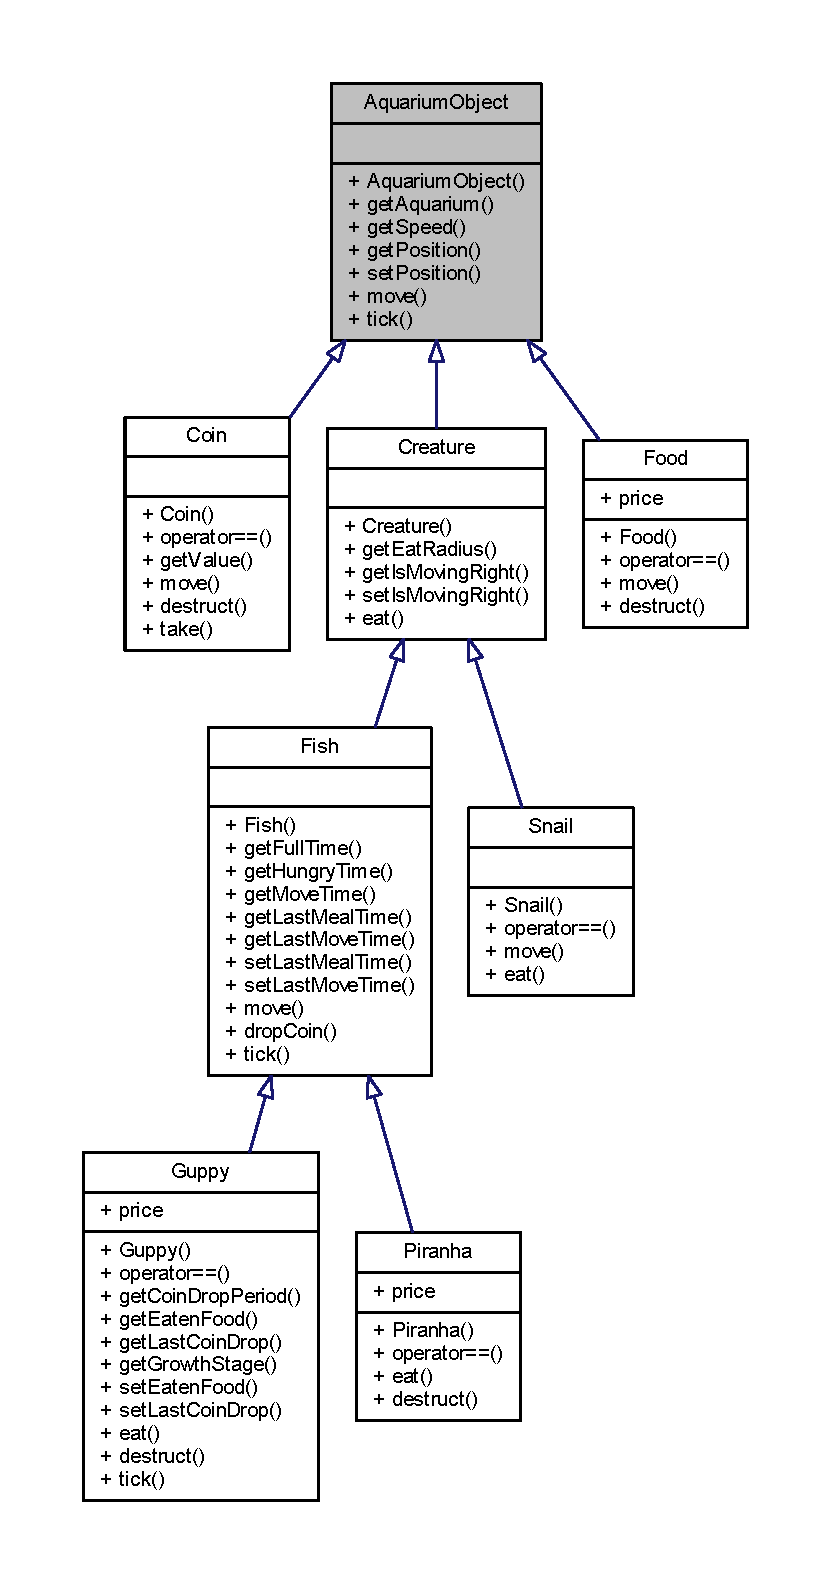
\includegraphics[height=550pt]{class_aquarium_object__inherit__graph}
\end{center}
\end{figure}


Collaboration diagram for Aquarium\+Object\+:\nopagebreak
\begin{figure}[H]
\begin{center}
\leavevmode
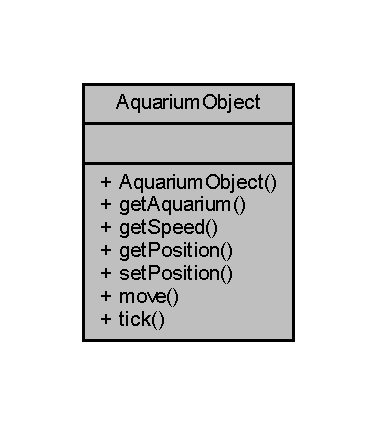
\includegraphics[width=181pt]{class_aquarium_object__coll__graph}
\end{center}
\end{figure}
\subsection*{Public Member Functions}
\begin{DoxyCompactItemize}
\item 
\mbox{\hyperlink{class_aquarium_object_aebe6958a63cab1a4277006d335d3c968}{Aquarium\+Object}} (\mbox{\hyperlink{class_aquarium}{Aquarium}} \&\+\_\+aquarium, float \+\_\+speed, \mbox{\hyperlink{struct_vector2}{Vector2}} \+\_\+position)
\begin{DoxyCompactList}\small\item\em Constructor. \end{DoxyCompactList}\item 
\mbox{\hyperlink{class_aquarium}{Aquarium}} \& \mbox{\hyperlink{class_aquarium_object_a229f2c41d3aa352bcbd7b994dd540f97}{get\+Aquarium}} () const
\begin{DoxyCompactList}\small\item\em Return reference to aquarium of this \mbox{\hyperlink{class_aquarium_object}{Aquarium\+Object}}. \end{DoxyCompactList}\item 
float \mbox{\hyperlink{class_aquarium_object_a0e554167f04a77e452d5714d31fadada}{get\+Speed}} () const
\begin{DoxyCompactList}\small\item\em Return speed. \end{DoxyCompactList}\item 
\mbox{\hyperlink{struct_vector2}{Vector2}} \mbox{\hyperlink{class_aquarium_object_aed4986687e54beb0ce780a9cafbda990}{get\+Position}} () const
\begin{DoxyCompactList}\small\item\em Return position. \end{DoxyCompactList}\item 
void \mbox{\hyperlink{class_aquarium_object_a2ec88f59595aec6ad788b90e9896b9b9}{set\+Position}} (\mbox{\hyperlink{struct_vector2}{Vector2}} \+\_\+position)
\begin{DoxyCompactList}\small\item\em Set position. \end{DoxyCompactList}\item 
virtual void \mbox{\hyperlink{class_aquarium_object_a42c4de640f89ac8aebc26b7618578575}{move}} ()=0
\begin{DoxyCompactList}\small\item\em Abstract function of move. \end{DoxyCompactList}\item 
virtual void \mbox{\hyperlink{class_aquarium_object_a3a8269dfe29631656916cce254e77059}{tick}} ()
\begin{DoxyCompactList}\small\item\em Do one game time unit\+: moves. \end{DoxyCompactList}\end{DoxyCompactItemize}


\subsection{Constructor \& Destructor Documentation}
\mbox{\Hypertarget{class_aquarium_object_aebe6958a63cab1a4277006d335d3c968}\label{class_aquarium_object_aebe6958a63cab1a4277006d335d3c968}} 
\index{Aquarium\+Object@{Aquarium\+Object}!Aquarium\+Object@{Aquarium\+Object}}
\index{Aquarium\+Object@{Aquarium\+Object}!Aquarium\+Object@{Aquarium\+Object}}
\subsubsection{\texorpdfstring{Aquarium\+Object()}{AquariumObject()}}
{\footnotesize\ttfamily Aquarium\+Object\+::\+Aquarium\+Object (\begin{DoxyParamCaption}\item[{\mbox{\hyperlink{class_aquarium}{Aquarium}} \&}]{\+\_\+aquarium,  }\item[{float}]{\+\_\+speed,  }\item[{\mbox{\hyperlink{struct_vector2}{Vector2}}}]{\+\_\+position }\end{DoxyParamCaption})}



Constructor. 



\subsection{Member Function Documentation}
\mbox{\Hypertarget{class_aquarium_object_a229f2c41d3aa352bcbd7b994dd540f97}\label{class_aquarium_object_a229f2c41d3aa352bcbd7b994dd540f97}} 
\index{Aquarium\+Object@{Aquarium\+Object}!get\+Aquarium@{get\+Aquarium}}
\index{get\+Aquarium@{get\+Aquarium}!Aquarium\+Object@{Aquarium\+Object}}
\subsubsection{\texorpdfstring{get\+Aquarium()}{getAquarium()}}
{\footnotesize\ttfamily \mbox{\hyperlink{class_aquarium}{Aquarium}} \& Aquarium\+Object\+::get\+Aquarium (\begin{DoxyParamCaption}{ }\end{DoxyParamCaption}) const}



Return reference to aquarium of this \mbox{\hyperlink{class_aquarium_object}{Aquarium\+Object}}. 

\mbox{\Hypertarget{class_aquarium_object_aed4986687e54beb0ce780a9cafbda990}\label{class_aquarium_object_aed4986687e54beb0ce780a9cafbda990}} 
\index{Aquarium\+Object@{Aquarium\+Object}!get\+Position@{get\+Position}}
\index{get\+Position@{get\+Position}!Aquarium\+Object@{Aquarium\+Object}}
\subsubsection{\texorpdfstring{get\+Position()}{getPosition()}}
{\footnotesize\ttfamily \mbox{\hyperlink{struct_vector2}{Vector2}} Aquarium\+Object\+::get\+Position (\begin{DoxyParamCaption}{ }\end{DoxyParamCaption}) const}



Return position. 

\mbox{\Hypertarget{class_aquarium_object_a0e554167f04a77e452d5714d31fadada}\label{class_aquarium_object_a0e554167f04a77e452d5714d31fadada}} 
\index{Aquarium\+Object@{Aquarium\+Object}!get\+Speed@{get\+Speed}}
\index{get\+Speed@{get\+Speed}!Aquarium\+Object@{Aquarium\+Object}}
\subsubsection{\texorpdfstring{get\+Speed()}{getSpeed()}}
{\footnotesize\ttfamily float Aquarium\+Object\+::get\+Speed (\begin{DoxyParamCaption}{ }\end{DoxyParamCaption}) const}



Return speed. 

\mbox{\Hypertarget{class_aquarium_object_a42c4de640f89ac8aebc26b7618578575}\label{class_aquarium_object_a42c4de640f89ac8aebc26b7618578575}} 
\index{Aquarium\+Object@{Aquarium\+Object}!move@{move}}
\index{move@{move}!Aquarium\+Object@{Aquarium\+Object}}
\subsubsection{\texorpdfstring{move()}{move()}}
{\footnotesize\ttfamily virtual void Aquarium\+Object\+::move (\begin{DoxyParamCaption}{ }\end{DoxyParamCaption})\hspace{0.3cm}{\ttfamily [pure virtual]}}



Abstract function of move. 



Implemented in \mbox{\hyperlink{class_fish_a1a18368573aab3b14a83aaf2424630ec}{Fish}}, \mbox{\hyperlink{class_coin_ab62bca5834489b9b483deaa3ca3470e9}{Coin}}, \mbox{\hyperlink{class_food_afb37f87b673df87697665ae82b6da0da}{Food}}, and \mbox{\hyperlink{class_snail_af5892ec122d9199480c813b74488256b}{Snail}}.

\mbox{\Hypertarget{class_aquarium_object_a2ec88f59595aec6ad788b90e9896b9b9}\label{class_aquarium_object_a2ec88f59595aec6ad788b90e9896b9b9}} 
\index{Aquarium\+Object@{Aquarium\+Object}!set\+Position@{set\+Position}}
\index{set\+Position@{set\+Position}!Aquarium\+Object@{Aquarium\+Object}}
\subsubsection{\texorpdfstring{set\+Position()}{setPosition()}}
{\footnotesize\ttfamily void Aquarium\+Object\+::set\+Position (\begin{DoxyParamCaption}\item[{\mbox{\hyperlink{struct_vector2}{Vector2}}}]{\+\_\+position }\end{DoxyParamCaption})}



Set position. 

\mbox{\Hypertarget{class_aquarium_object_a3a8269dfe29631656916cce254e77059}\label{class_aquarium_object_a3a8269dfe29631656916cce254e77059}} 
\index{Aquarium\+Object@{Aquarium\+Object}!tick@{tick}}
\index{tick@{tick}!Aquarium\+Object@{Aquarium\+Object}}
\subsubsection{\texorpdfstring{tick()}{tick()}}
{\footnotesize\ttfamily void Aquarium\+Object\+::tick (\begin{DoxyParamCaption}{ }\end{DoxyParamCaption})\hspace{0.3cm}{\ttfamily [virtual]}}



Do one game time unit\+: moves. 



Reimplemented in \mbox{\hyperlink{class_guppy_ab2f219fa29b0d22ee9702a55fede519b}{Guppy}}, and \mbox{\hyperlink{class_fish_aa49a70677a400c471b1e3db5d8f1881e}{Fish}}.



The documentation for this class was generated from the following files\+:\begin{DoxyCompactItemize}
\item 
\mbox{\hyperlink{_aquarium_object_8hpp}{Aquarium\+Object.\+hpp}}\item 
\mbox{\hyperlink{_aquarium_object_8cpp}{Aquarium\+Object.\+cpp}}\end{DoxyCompactItemize}

\hypertarget{class_coin}{}\section{Coin Class Reference}
\label{class_coin}\index{Coin@{Coin}}


{\ttfamily \#include $<$Coin.\+hpp$>$}



Inheritance diagram for Coin\+:
\nopagebreak
\begin{figure}[H]
\begin{center}
\leavevmode
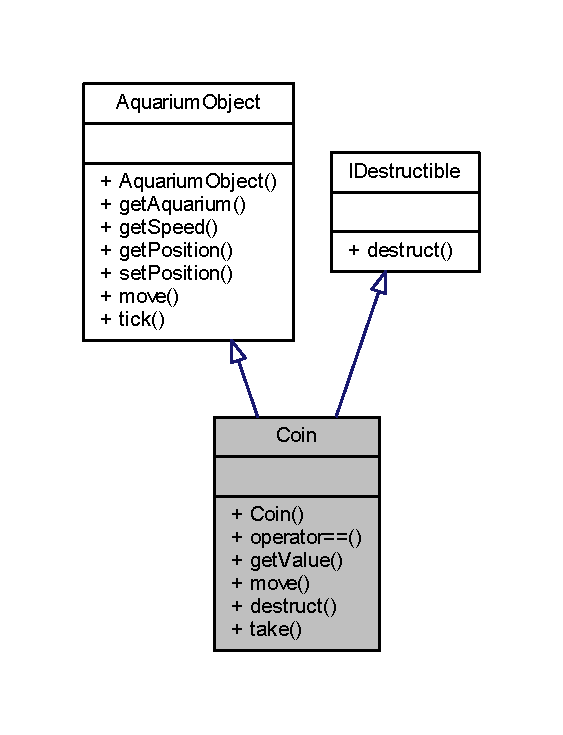
\includegraphics[width=270pt]{class_coin__inherit__graph}
\end{center}
\end{figure}


Collaboration diagram for Coin\+:
\nopagebreak
\begin{figure}[H]
\begin{center}
\leavevmode
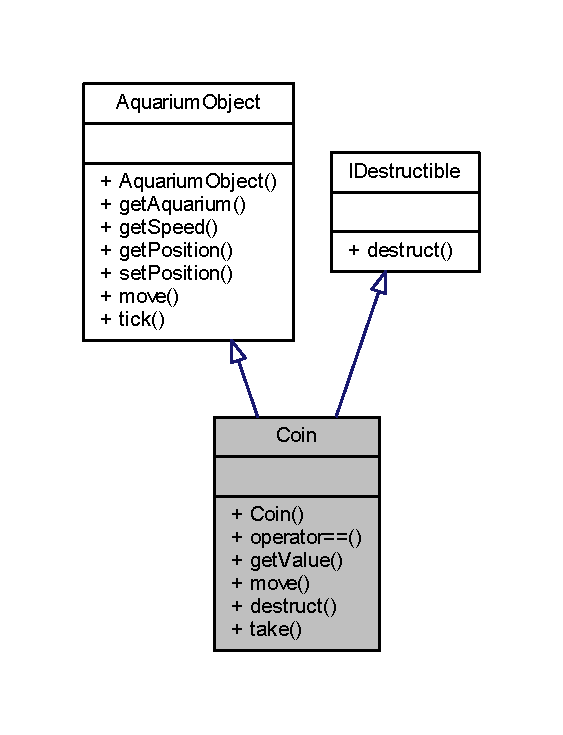
\includegraphics[width=270pt]{class_coin__coll__graph}
\end{center}
\end{figure}
\subsection*{Public Member Functions}
\begin{DoxyCompactItemize}
\item 
\mbox{\hyperlink{class_coin_a5aa05323e2dab5f755e283d66ef1aae8}{Coin}} (\mbox{\hyperlink{class_aquarium}{Aquarium}} \&\+\_\+aquarium, \mbox{\hyperlink{struct_vector2}{Vector2}} \+\_\+position, int \+\_\+value)
\begin{DoxyCompactList}\small\item\em Constructor. \end{DoxyCompactList}\item 
bool \mbox{\hyperlink{class_coin_a803072934a3da4010352955208e14c4e}{operator==}} (const \mbox{\hyperlink{class_coin}{Coin}} \&other) const
\begin{DoxyCompactList}\small\item\em Reference comparison. \end{DoxyCompactList}\item 
int \mbox{\hyperlink{class_coin_a53c8bf65afdde1422cfda51d753d74b7}{get\+Value}} () const
\begin{DoxyCompactList}\small\item\em Return coin\textquotesingle{}s value. \end{DoxyCompactList}\item 
void \mbox{\hyperlink{class_coin_ab62bca5834489b9b483deaa3ca3470e9}{move}} ()
\begin{DoxyCompactList}\small\item\em Move this coin to the bottom. \end{DoxyCompactList}\item 
void \mbox{\hyperlink{class_coin_a16c42ef0d21f50bb08d4099d82b4ed57}{destruct}} ()
\begin{DoxyCompactList}\small\item\em Remove this coin from aquarium. \end{DoxyCompactList}\item 
void \mbox{\hyperlink{class_coin_abdc8520a89656c688cc70cffa14265ca}{take}} ()
\begin{DoxyCompactList}\small\item\em Increase money by value. \end{DoxyCompactList}\end{DoxyCompactItemize}


\subsection{Constructor \& Destructor Documentation}
\mbox{\Hypertarget{class_coin_a5aa05323e2dab5f755e283d66ef1aae8}\label{class_coin_a5aa05323e2dab5f755e283d66ef1aae8}} 
\index{Coin@{Coin}!Coin@{Coin}}
\index{Coin@{Coin}!Coin@{Coin}}
\subsubsection{\texorpdfstring{Coin()}{Coin()}}
{\footnotesize\ttfamily Coin\+::\+Coin (\begin{DoxyParamCaption}\item[{\mbox{\hyperlink{class_aquarium}{Aquarium}} \&}]{\+\_\+aquarium,  }\item[{\mbox{\hyperlink{struct_vector2}{Vector2}}}]{\+\_\+position,  }\item[{int}]{\+\_\+value }\end{DoxyParamCaption})}



Constructor. 



\subsection{Member Function Documentation}
\mbox{\Hypertarget{class_coin_a16c42ef0d21f50bb08d4099d82b4ed57}\label{class_coin_a16c42ef0d21f50bb08d4099d82b4ed57}} 
\index{Coin@{Coin}!destruct@{destruct}}
\index{destruct@{destruct}!Coin@{Coin}}
\subsubsection{\texorpdfstring{destruct()}{destruct()}}
{\footnotesize\ttfamily void Coin\+::destruct (\begin{DoxyParamCaption}{ }\end{DoxyParamCaption})\hspace{0.3cm}{\ttfamily [virtual]}}



Remove this coin from aquarium. 



Implements \mbox{\hyperlink{class_i_destructible_a63016d1bb4daa0a726fc8add9a0be62d}{I\+Destructible}}.

\mbox{\Hypertarget{class_coin_a53c8bf65afdde1422cfda51d753d74b7}\label{class_coin_a53c8bf65afdde1422cfda51d753d74b7}} 
\index{Coin@{Coin}!get\+Value@{get\+Value}}
\index{get\+Value@{get\+Value}!Coin@{Coin}}
\subsubsection{\texorpdfstring{get\+Value()}{getValue()}}
{\footnotesize\ttfamily int Coin\+::get\+Value (\begin{DoxyParamCaption}{ }\end{DoxyParamCaption}) const}



Return coin\textquotesingle{}s value. 

\mbox{\Hypertarget{class_coin_ab62bca5834489b9b483deaa3ca3470e9}\label{class_coin_ab62bca5834489b9b483deaa3ca3470e9}} 
\index{Coin@{Coin}!move@{move}}
\index{move@{move}!Coin@{Coin}}
\subsubsection{\texorpdfstring{move()}{move()}}
{\footnotesize\ttfamily void Coin\+::move (\begin{DoxyParamCaption}{ }\end{DoxyParamCaption})\hspace{0.3cm}{\ttfamily [virtual]}}



Move this coin to the bottom. 



Implements \mbox{\hyperlink{class_aquarium_object_a42c4de640f89ac8aebc26b7618578575}{Aquarium\+Object}}.

\mbox{\Hypertarget{class_coin_a803072934a3da4010352955208e14c4e}\label{class_coin_a803072934a3da4010352955208e14c4e}} 
\index{Coin@{Coin}!operator==@{operator==}}
\index{operator==@{operator==}!Coin@{Coin}}
\subsubsection{\texorpdfstring{operator==()}{operator==()}}
{\footnotesize\ttfamily bool Coin\+::operator== (\begin{DoxyParamCaption}\item[{const \mbox{\hyperlink{class_coin}{Coin}} \&}]{other }\end{DoxyParamCaption}) const}



Reference comparison. 

\mbox{\Hypertarget{class_coin_abdc8520a89656c688cc70cffa14265ca}\label{class_coin_abdc8520a89656c688cc70cffa14265ca}} 
\index{Coin@{Coin}!take@{take}}
\index{take@{take}!Coin@{Coin}}
\subsubsection{\texorpdfstring{take()}{take()}}
{\footnotesize\ttfamily void Coin\+::take (\begin{DoxyParamCaption}{ }\end{DoxyParamCaption})}



Increase money by value. 



The documentation for this class was generated from the following files\+:\begin{DoxyCompactItemize}
\item 
\mbox{\hyperlink{_coin_8hpp}{Coin.\+hpp}}\item 
\mbox{\hyperlink{_coin_8cpp}{Coin.\+cpp}}\end{DoxyCompactItemize}

\hypertarget{class_creature}{}\section{Creature Class Reference}
\label{class_creature}\index{Creature@{Creature}}


{\ttfamily \#include $<$Creature.\+hpp$>$}



Inheritance diagram for Creature\+:
% FIG 0


Collaboration diagram for Creature\+:
% FIG 1
\subsection*{Public Member Functions}
\begin{DoxyCompactItemize}
\item 
\mbox{\hyperlink{class_creature_ab12ad708dcef6c9cd0509f6769a6329a}{Creature}} (\mbox{\hyperlink{class_aquarium}{Aquarium}} \&\+\_\+aquarium, float \+\_\+speed, \mbox{\hyperlink{struct_vector2}{Vector2}} \+\_\+position, float \+\_\+eat\+Radius)
\item 
float \mbox{\hyperlink{class_creature_a24e52cedddd872269f83671c9a6f6925}{get\+Eat\+Radius}} () const
\item 
bool \mbox{\hyperlink{class_creature_a63abd829cfac5d57425452b39f2a21b7}{get\+Is\+Moving\+Right}} () const
\item 
void \mbox{\hyperlink{class_creature_a7b222797d42b668ebf2a02eef51feaf8}{set\+Is\+Moving\+Right}} (bool \+\_\+is\+Moving\+Right)
\item 
virtual \mbox{\hyperlink{struct_vector2}{Vector2}} \mbox{\hyperlink{class_creature_a0d531a4c04c1021833ddb0e48864dbf4}{eat}} ()=0
\end{DoxyCompactItemize}


\subsection{Constructor \& Destructor Documentation}
\mbox{\Hypertarget{class_creature_ab12ad708dcef6c9cd0509f6769a6329a}\label{class_creature_ab12ad708dcef6c9cd0509f6769a6329a}} 
\index{Creature@{Creature}!Creature@{Creature}}
\index{Creature@{Creature}!Creature@{Creature}}
\subsubsection{\texorpdfstring{Creature()}{Creature()}}
{\footnotesize\ttfamily Creature\+::\+Creature (\begin{DoxyParamCaption}\item[{\mbox{\hyperlink{class_aquarium}{Aquarium}} \&}]{\+\_\+aquarium,  }\item[{float}]{\+\_\+speed,  }\item[{\mbox{\hyperlink{struct_vector2}{Vector2}}}]{\+\_\+position,  }\item[{float}]{\+\_\+eat\+Radius }\end{DoxyParamCaption})}



\subsection{Member Function Documentation}
\mbox{\Hypertarget{class_creature_a0d531a4c04c1021833ddb0e48864dbf4}\label{class_creature_a0d531a4c04c1021833ddb0e48864dbf4}} 
\index{Creature@{Creature}!eat@{eat}}
\index{eat@{eat}!Creature@{Creature}}
\subsubsection{\texorpdfstring{eat()}{eat()}}
{\footnotesize\ttfamily virtual \mbox{\hyperlink{struct_vector2}{Vector2}} Creature\+::eat (\begin{DoxyParamCaption}{ }\end{DoxyParamCaption})\hspace{0.3cm}{\ttfamily [pure virtual]}}



Implemented in \mbox{\hyperlink{class_guppy_aaeab888b423fd0ea3cc911b974b04f48}{Guppy}}, \mbox{\hyperlink{class_snail_a0905a469c6333970b8246abca37795f1}{Snail}}, and \mbox{\hyperlink{class_piranha_a125847235bdbd0e8c676dcada0d86c14}{Piranha}}.

\mbox{\Hypertarget{class_creature_a24e52cedddd872269f83671c9a6f6925}\label{class_creature_a24e52cedddd872269f83671c9a6f6925}} 
\index{Creature@{Creature}!get\+Eat\+Radius@{get\+Eat\+Radius}}
\index{get\+Eat\+Radius@{get\+Eat\+Radius}!Creature@{Creature}}
\subsubsection{\texorpdfstring{get\+Eat\+Radius()}{getEatRadius()}}
{\footnotesize\ttfamily float Creature\+::get\+Eat\+Radius (\begin{DoxyParamCaption}{ }\end{DoxyParamCaption}) const}

\mbox{\Hypertarget{class_creature_a63abd829cfac5d57425452b39f2a21b7}\label{class_creature_a63abd829cfac5d57425452b39f2a21b7}} 
\index{Creature@{Creature}!get\+Is\+Moving\+Right@{get\+Is\+Moving\+Right}}
\index{get\+Is\+Moving\+Right@{get\+Is\+Moving\+Right}!Creature@{Creature}}
\subsubsection{\texorpdfstring{get\+Is\+Moving\+Right()}{getIsMovingRight()}}
{\footnotesize\ttfamily bool Creature\+::get\+Is\+Moving\+Right (\begin{DoxyParamCaption}{ }\end{DoxyParamCaption}) const}

\mbox{\Hypertarget{class_creature_a7b222797d42b668ebf2a02eef51feaf8}\label{class_creature_a7b222797d42b668ebf2a02eef51feaf8}} 
\index{Creature@{Creature}!set\+Is\+Moving\+Right@{set\+Is\+Moving\+Right}}
\index{set\+Is\+Moving\+Right@{set\+Is\+Moving\+Right}!Creature@{Creature}}
\subsubsection{\texorpdfstring{set\+Is\+Moving\+Right()}{setIsMovingRight()}}
{\footnotesize\ttfamily void Creature\+::set\+Is\+Moving\+Right (\begin{DoxyParamCaption}\item[{bool}]{\+\_\+is\+Moving\+Right }\end{DoxyParamCaption})}



The documentation for this class was generated from the following files\+:\begin{DoxyCompactItemize}
\item 
\mbox{\hyperlink{_creature_8hpp}{Creature.\+hpp}}\item 
\mbox{\hyperlink{_creature_8cpp}{Creature.\+cpp}}\end{DoxyCompactItemize}

\hypertarget{struct_element_list}{}\section{Element\+List$<$ T $>$ Struct Template Reference}
\label{struct_element_list}\index{Element\+List$<$ T $>$@{Element\+List$<$ T $>$}}


{\ttfamily \#include $<$Linked\+List.\+hpp$>$}



Inheritance diagram for Element\+List$<$ T $>$\+:
\nopagebreak
\begin{figure}[H]
\begin{center}
\leavevmode
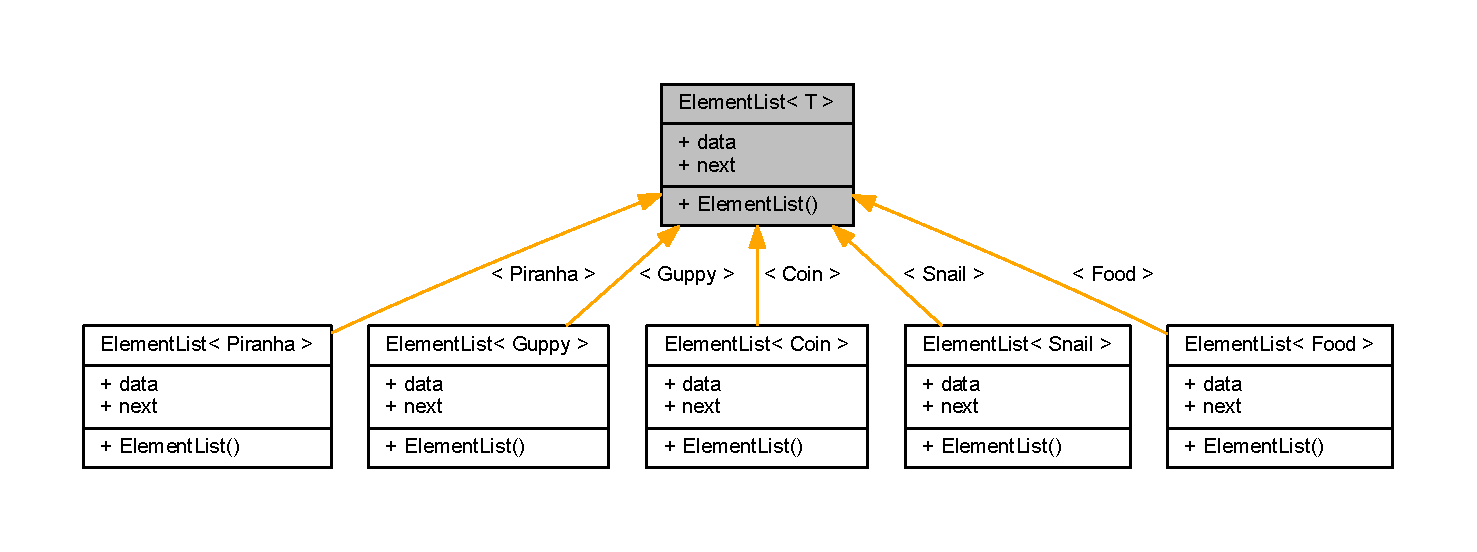
\includegraphics[width=350pt]{struct_element_list__inherit__graph}
\end{center}
\end{figure}


Collaboration diagram for Element\+List$<$ T $>$\+:
\nopagebreak
\begin{figure}[H]
\begin{center}
\leavevmode
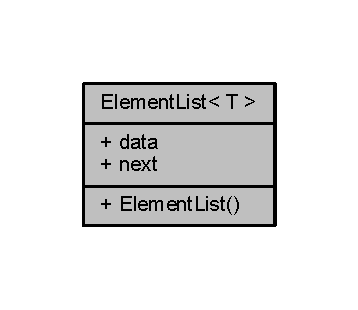
\includegraphics[width=172pt]{struct_element_list__coll__graph}
\end{center}
\end{figure}
\subsection*{Public Member Functions}
\begin{DoxyCompactItemize}
\item 
\mbox{\hyperlink{struct_element_list_a2f2c3bfdd0cda10f2e50f8f04758b52a}{Element\+List}} (const T \&element)
\end{DoxyCompactItemize}
\subsection*{Public Attributes}
\begin{DoxyCompactItemize}
\item 
T \mbox{\hyperlink{struct_element_list_a4c3bbe183d5a854d51e193b21075c884}{data}}
\item 
\mbox{\hyperlink{struct_element_list}{Element\+List}}$<$ T $>$ $\ast$ \mbox{\hyperlink{struct_element_list_ae15f34d3109949237cf3ba98a074d402}{next}}
\end{DoxyCompactItemize}


\subsection{Constructor \& Destructor Documentation}
\mbox{\Hypertarget{struct_element_list_a2f2c3bfdd0cda10f2e50f8f04758b52a}\label{struct_element_list_a2f2c3bfdd0cda10f2e50f8f04758b52a}} 
\index{Element\+List@{Element\+List}!Element\+List@{Element\+List}}
\index{Element\+List@{Element\+List}!Element\+List@{Element\+List}}
\subsubsection{\texorpdfstring{Element\+List()}{ElementList()}}
{\footnotesize\ttfamily template$<$typename T$>$ \\
\mbox{\hyperlink{struct_element_list}{Element\+List}}$<$ T $>$\+::\mbox{\hyperlink{struct_element_list}{Element\+List}} (\begin{DoxyParamCaption}\item[{const T \&}]{element }\end{DoxyParamCaption})\hspace{0.3cm}{\ttfamily [inline]}}



\subsection{Member Data Documentation}
\mbox{\Hypertarget{struct_element_list_a4c3bbe183d5a854d51e193b21075c884}\label{struct_element_list_a4c3bbe183d5a854d51e193b21075c884}} 
\index{Element\+List@{Element\+List}!data@{data}}
\index{data@{data}!Element\+List@{Element\+List}}
\subsubsection{\texorpdfstring{data}{data}}
{\footnotesize\ttfamily template$<$typename T$>$ \\
T \mbox{\hyperlink{struct_element_list}{Element\+List}}$<$ T $>$\+::data}

\mbox{\Hypertarget{struct_element_list_ae15f34d3109949237cf3ba98a074d402}\label{struct_element_list_ae15f34d3109949237cf3ba98a074d402}} 
\index{Element\+List@{Element\+List}!next@{next}}
\index{next@{next}!Element\+List@{Element\+List}}
\subsubsection{\texorpdfstring{next}{next}}
{\footnotesize\ttfamily template$<$typename T$>$ \\
\mbox{\hyperlink{struct_element_list}{Element\+List}}$<$T$>$$\ast$ \mbox{\hyperlink{struct_element_list}{Element\+List}}$<$ T $>$\+::next}



The documentation for this struct was generated from the following file\+:\begin{DoxyCompactItemize}
\item 
\mbox{\hyperlink{_linked_list_8hpp}{Linked\+List.\+hpp}}\end{DoxyCompactItemize}

\hypertarget{class_fish}{}\section{Fish Class Reference}
\label{class_fish}\index{Fish@{Fish}}


Inheritance diagram for Fish\+:
\nopagebreak
\begin{figure}[H]
\begin{center}
\leavevmode
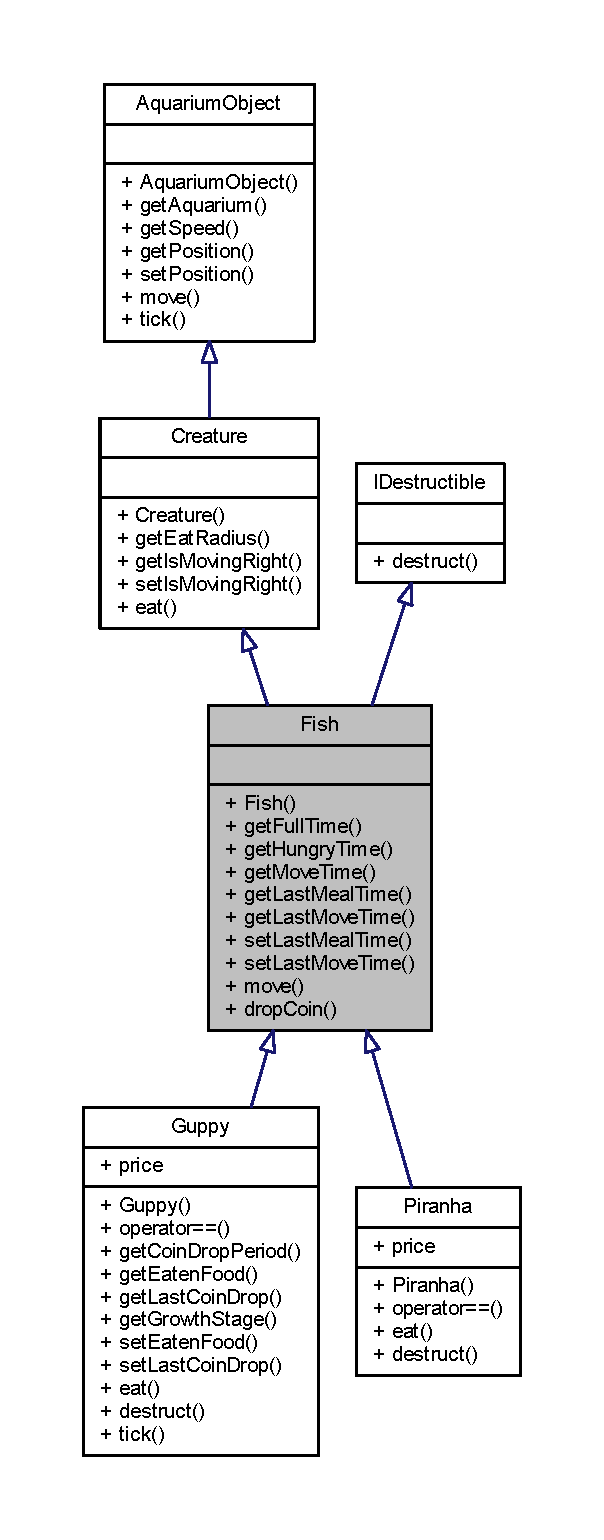
\includegraphics[height=550pt]{class_fish__inherit__graph}
\end{center}
\end{figure}


Collaboration diagram for Fish\+:
\nopagebreak
\begin{figure}[H]
\begin{center}
\leavevmode
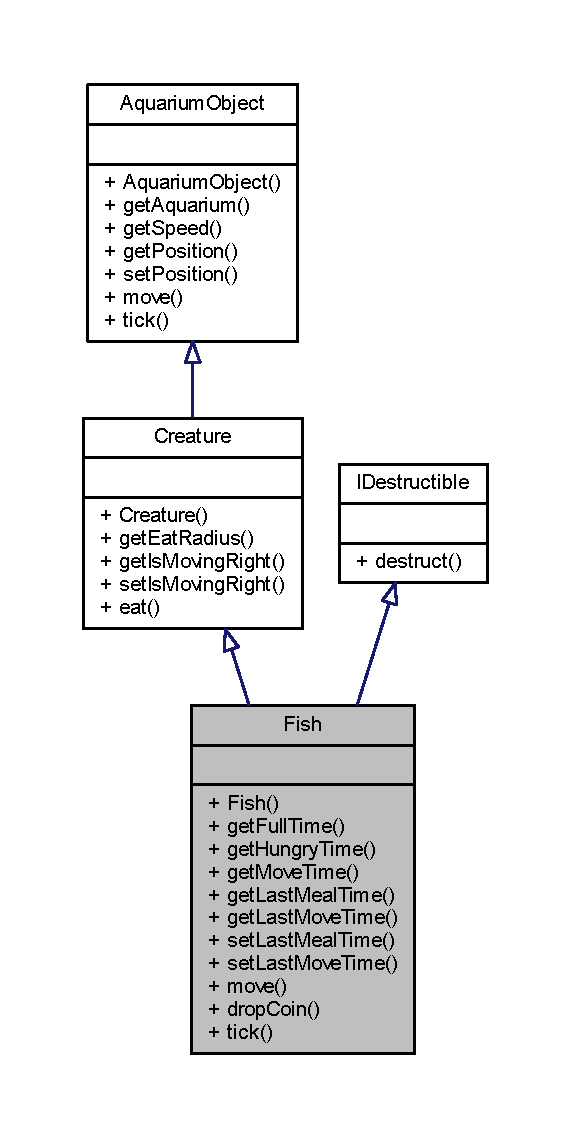
\includegraphics[width=274pt]{class_fish__coll__graph}
\end{center}
\end{figure}
\subsection*{Public Member Functions}
\begin{DoxyCompactItemize}
\item 
\mbox{\hyperlink{class_fish_adc54cd97ba29e2bce4f102f2d8cd3b99}{Fish}} (\mbox{\hyperlink{class_aquarium}{Aquarium}} aquarium, float speed, float eat\+Radius)
\item 
int \mbox{\hyperlink{class_fish_ad8e2387d09b2a4b10f3581797551f82c}{get\+Full\+Time}} ()
\item 
int \mbox{\hyperlink{class_fish_af9203b3a4949cac453fc8d18355af9b5}{get\+Hungry\+Time}} ()
\item 
int \mbox{\hyperlink{class_fish_af967adfd2d8b4486175131509fcf541b}{get\+Move\+Time}} ()
\item 
int \mbox{\hyperlink{class_fish_a84aaee65d812cd3f8357c9173ec13b75}{get\+Last\+Meal\+Time}} ()
\item 
int \mbox{\hyperlink{class_fish_a57dcae78fad400c6b8e09f1443acf491}{get\+Last\+Move\+Time}} ()
\item 
void \mbox{\hyperlink{class_fish_aedb34efda974a200bd6b929e26955080}{set\+Last\+Meal\+Time}} (int last\+Meal\+Time)
\item 
void \mbox{\hyperlink{class_fish_a5c8ba21e13233735384d25a521a6b022}{set\+Last\+Move\+Time}} (int last\+Move\+Time)
\item 
void \mbox{\hyperlink{class_fish_ad624caf044894e5c4350cd69ef846833}{move}} ()
\item 
void \mbox{\hyperlink{class_fish_a7ce58f40d4cfeb6472788af5627252c1}{drop\+Coin}} (int value)
\item 
void \mbox{\hyperlink{class_fish_aefe1a78dd5e5bf6a4f152c948d701a09}{tick}} ()
\end{DoxyCompactItemize}


\subsection{Constructor \& Destructor Documentation}
\mbox{\Hypertarget{class_fish_adc54cd97ba29e2bce4f102f2d8cd3b99}\label{class_fish_adc54cd97ba29e2bce4f102f2d8cd3b99}} 
\index{Fish@{Fish}!Fish@{Fish}}
\index{Fish@{Fish}!Fish@{Fish}}
\subsubsection{\texorpdfstring{Fish()}{Fish()}}
{\footnotesize\ttfamily Fish.\+Fish (\begin{DoxyParamCaption}\item[{\mbox{\hyperlink{class_aquarium}{Aquarium}}}]{aquarium,  }\item[{float}]{speed,  }\item[{float}]{eat\+Radius }\end{DoxyParamCaption})\hspace{0.3cm}{\ttfamily [inline]}}

Constructor\+: instantiate fish at random position 
\begin{DoxyParams}{Parameters}
{\em aquarium} & object aquarium which will be added by fish and will be initialized \\
\hline
{\em speed} & fish speed which will be initialized \\
\hline
{\em eat\+Radius} & fish eat radius which will be initialized \\
\hline
\end{DoxyParams}


\subsection{Member Function Documentation}
\mbox{\Hypertarget{class_fish_a7ce58f40d4cfeb6472788af5627252c1}\label{class_fish_a7ce58f40d4cfeb6472788af5627252c1}} 
\index{Fish@{Fish}!drop\+Coin@{drop\+Coin}}
\index{drop\+Coin@{drop\+Coin}!Fish@{Fish}}
\subsubsection{\texorpdfstring{drop\+Coin()}{dropCoin()}}
{\footnotesize\ttfamily void Fish.\+drop\+Coin (\begin{DoxyParamCaption}\item[{int}]{value }\end{DoxyParamCaption})\hspace{0.3cm}{\ttfamily [inline]}}

Drop coin from this fish 
\begin{DoxyParams}{Parameters}
{\em value} & the coin\textquotesingle{}s value \\
\hline
\end{DoxyParams}
\mbox{\Hypertarget{class_fish_ad8e2387d09b2a4b10f3581797551f82c}\label{class_fish_ad8e2387d09b2a4b10f3581797551f82c}} 
\index{Fish@{Fish}!get\+Full\+Time@{get\+Full\+Time}}
\index{get\+Full\+Time@{get\+Full\+Time}!Fish@{Fish}}
\subsubsection{\texorpdfstring{get\+Full\+Time()}{getFullTime()}}
{\footnotesize\ttfamily int Fish.\+get\+Full\+Time (\begin{DoxyParamCaption}{ }\end{DoxyParamCaption})\hspace{0.3cm}{\ttfamily [inline]}}

Get the duration of this fish full before hungry again \begin{DoxyReturn}{Returns}
the duration of this fish full before hungry again 
\end{DoxyReturn}
\mbox{\Hypertarget{class_fish_af9203b3a4949cac453fc8d18355af9b5}\label{class_fish_af9203b3a4949cac453fc8d18355af9b5}} 
\index{Fish@{Fish}!get\+Hungry\+Time@{get\+Hungry\+Time}}
\index{get\+Hungry\+Time@{get\+Hungry\+Time}!Fish@{Fish}}
\subsubsection{\texorpdfstring{get\+Hungry\+Time()}{getHungryTime()}}
{\footnotesize\ttfamily int Fish.\+get\+Hungry\+Time (\begin{DoxyParamCaption}{ }\end{DoxyParamCaption})\hspace{0.3cm}{\ttfamily [inline]}}

Get the duration of this fish hungry before it dies \begin{DoxyReturn}{Returns}
the duration of this fish hungry before it dies 
\end{DoxyReturn}
\mbox{\Hypertarget{class_fish_a84aaee65d812cd3f8357c9173ec13b75}\label{class_fish_a84aaee65d812cd3f8357c9173ec13b75}} 
\index{Fish@{Fish}!get\+Last\+Meal\+Time@{get\+Last\+Meal\+Time}}
\index{get\+Last\+Meal\+Time@{get\+Last\+Meal\+Time}!Fish@{Fish}}
\subsubsection{\texorpdfstring{get\+Last\+Meal\+Time()}{getLastMealTime()}}
{\footnotesize\ttfamily int Fish.\+get\+Last\+Meal\+Time (\begin{DoxyParamCaption}{ }\end{DoxyParamCaption})\hspace{0.3cm}{\ttfamily [inline]}}

Get the last time this fish eats \begin{DoxyReturn}{Returns}
the last time this fish eats 
\end{DoxyReturn}
\mbox{\Hypertarget{class_fish_a57dcae78fad400c6b8e09f1443acf491}\label{class_fish_a57dcae78fad400c6b8e09f1443acf491}} 
\index{Fish@{Fish}!get\+Last\+Move\+Time@{get\+Last\+Move\+Time}}
\index{get\+Last\+Move\+Time@{get\+Last\+Move\+Time}!Fish@{Fish}}
\subsubsection{\texorpdfstring{get\+Last\+Move\+Time()}{getLastMoveTime()}}
{\footnotesize\ttfamily int Fish.\+get\+Last\+Move\+Time (\begin{DoxyParamCaption}{ }\end{DoxyParamCaption})\hspace{0.3cm}{\ttfamily [inline]}}

Get the last time this fish moves \begin{DoxyReturn}{Returns}
the last time this fish moves 
\end{DoxyReturn}
\mbox{\Hypertarget{class_fish_af967adfd2d8b4486175131509fcf541b}\label{class_fish_af967adfd2d8b4486175131509fcf541b}} 
\index{Fish@{Fish}!get\+Move\+Time@{get\+Move\+Time}}
\index{get\+Move\+Time@{get\+Move\+Time}!Fish@{Fish}}
\subsubsection{\texorpdfstring{get\+Move\+Time()}{getMoveTime()}}
{\footnotesize\ttfamily int Fish.\+get\+Move\+Time (\begin{DoxyParamCaption}{ }\end{DoxyParamCaption})\hspace{0.3cm}{\ttfamily [inline]}}

Get the duration of this fish moving before changing direction \begin{DoxyReturn}{Returns}
the duration of this fish moving before changing direction 
\end{DoxyReturn}
\mbox{\Hypertarget{class_fish_ad624caf044894e5c4350cd69ef846833}\label{class_fish_ad624caf044894e5c4350cd69ef846833}} 
\index{Fish@{Fish}!move@{move}}
\index{move@{move}!Fish@{Fish}}
\subsubsection{\texorpdfstring{move()}{move()}}
{\footnotesize\ttfamily void Fish.\+move (\begin{DoxyParamCaption}{ }\end{DoxyParamCaption})\hspace{0.3cm}{\ttfamily [inline]}}

Move towards food if this fish is hungry and food exist, move randomly otherwise \mbox{\Hypertarget{class_fish_aedb34efda974a200bd6b929e26955080}\label{class_fish_aedb34efda974a200bd6b929e26955080}} 
\index{Fish@{Fish}!set\+Last\+Meal\+Time@{set\+Last\+Meal\+Time}}
\index{set\+Last\+Meal\+Time@{set\+Last\+Meal\+Time}!Fish@{Fish}}
\subsubsection{\texorpdfstring{set\+Last\+Meal\+Time()}{setLastMealTime()}}
{\footnotesize\ttfamily void Fish.\+set\+Last\+Meal\+Time (\begin{DoxyParamCaption}\item[{int}]{last\+Meal\+Time }\end{DoxyParamCaption})\hspace{0.3cm}{\ttfamily [inline]}}

Set the last time this fish eats 
\begin{DoxyParams}{Parameters}
{\em last\+Meal\+Time} & the last time this fish eats \\
\hline
\end{DoxyParams}
\mbox{\Hypertarget{class_fish_a5c8ba21e13233735384d25a521a6b022}\label{class_fish_a5c8ba21e13233735384d25a521a6b022}} 
\index{Fish@{Fish}!set\+Last\+Move\+Time@{set\+Last\+Move\+Time}}
\index{set\+Last\+Move\+Time@{set\+Last\+Move\+Time}!Fish@{Fish}}
\subsubsection{\texorpdfstring{set\+Last\+Move\+Time()}{setLastMoveTime()}}
{\footnotesize\ttfamily void Fish.\+set\+Last\+Move\+Time (\begin{DoxyParamCaption}\item[{int}]{last\+Move\+Time }\end{DoxyParamCaption})\hspace{0.3cm}{\ttfamily [inline]}}

Set the last time this fish moves 
\begin{DoxyParams}{Parameters}
{\em last\+Move\+Time} & the last time this fish moves \\
\hline
\end{DoxyParams}
\mbox{\Hypertarget{class_fish_aefe1a78dd5e5bf6a4f152c948d701a09}\label{class_fish_aefe1a78dd5e5bf6a4f152c948d701a09}} 
\index{Fish@{Fish}!tick@{tick}}
\index{tick@{tick}!Fish@{Fish}}
\subsubsection{\texorpdfstring{tick()}{tick()}}
{\footnotesize\ttfamily void Fish.\+tick (\begin{DoxyParamCaption}{ }\end{DoxyParamCaption})\hspace{0.3cm}{\ttfamily [inline]}}

Do one game time unit Dies if game\+Time is greater than or equals the last time this fish eats plus the duration of this fish full before hungry again plus the duration of this fish hungry before it dies 

The documentation for this class was generated from the following file\+:\begin{DoxyCompactItemize}
\item 
\mbox{\hyperlink{_fish_8java}{Fish.\+java}}\end{DoxyCompactItemize}

\hypertarget{class_food}{}\section{Food Class Reference}
\label{class_food}\index{Food@{Food}}


{\ttfamily \#include $<$Food.\+hpp$>$}



Inheritance diagram for Food\+:
\nopagebreak
\begin{figure}[H]
\begin{center}
\leavevmode
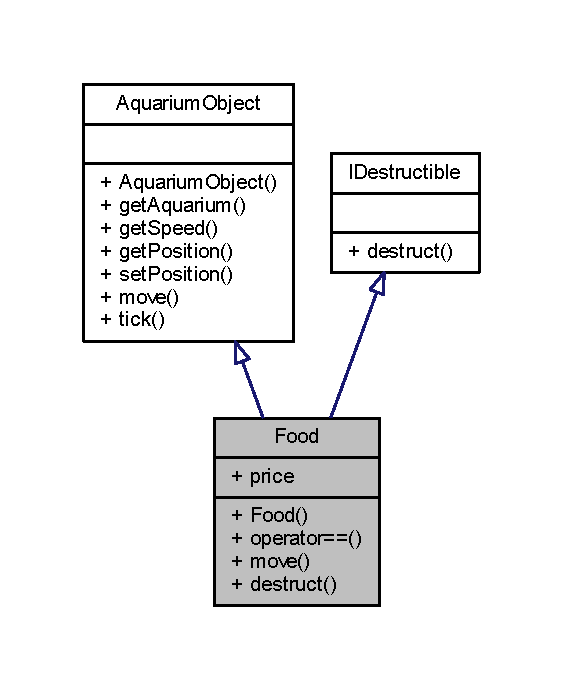
\includegraphics[width=270pt]{class_food__inherit__graph}
\end{center}
\end{figure}


Collaboration diagram for Food\+:
\nopagebreak
\begin{figure}[H]
\begin{center}
\leavevmode
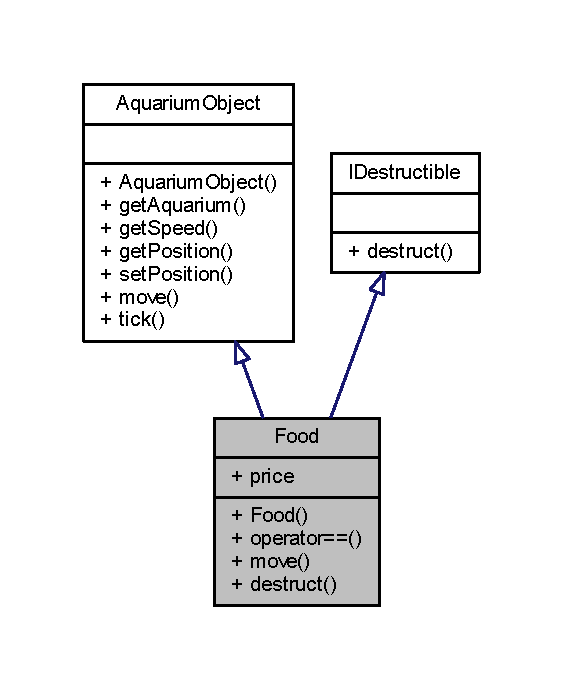
\includegraphics[width=270pt]{class_food__coll__graph}
\end{center}
\end{figure}
\subsection*{Public Member Functions}
\begin{DoxyCompactItemize}
\item 
\mbox{\hyperlink{class_food_ad36b16582fc56aa938f50870f5ec6b52}{Food}} (\mbox{\hyperlink{class_aquarium}{Aquarium}} \&\+\_\+aquarium, float x)
\begin{DoxyCompactList}\small\item\em Constructor\+: instantiate food on top of aquarium. \end{DoxyCompactList}\item 
bool \mbox{\hyperlink{class_food_a7199d2bd48ecae8ffbbf1be8a39c5311}{operator==}} (const \mbox{\hyperlink{class_food}{Food}} \&other) const
\begin{DoxyCompactList}\small\item\em Reference comparison. \end{DoxyCompactList}\item 
void \mbox{\hyperlink{class_food_afb37f87b673df87697665ae82b6da0da}{move}} ()
\begin{DoxyCompactList}\small\item\em Move this food to the bottom and destruct itself on touching aquarium\textquotesingle{}s floor. \end{DoxyCompactList}\item 
void \mbox{\hyperlink{class_food_a5e1bfe34f8a4f4ce60accc57212c95c8}{destruct}} ()
\begin{DoxyCompactList}\small\item\em Remove this food from aquarium. \end{DoxyCompactList}\end{DoxyCompactItemize}
\subsection*{Static Public Attributes}
\begin{DoxyCompactItemize}
\item 
static const int \mbox{\hyperlink{class_food_af54f2090e84e95fcdc95f5c2d93386df}{price}} = 5
\end{DoxyCompactItemize}


\subsection{Constructor \& Destructor Documentation}
\mbox{\Hypertarget{class_food_ad36b16582fc56aa938f50870f5ec6b52}\label{class_food_ad36b16582fc56aa938f50870f5ec6b52}} 
\index{Food@{Food}!Food@{Food}}
\index{Food@{Food}!Food@{Food}}
\subsubsection{\texorpdfstring{Food()}{Food()}}
{\footnotesize\ttfamily Food\+::\+Food (\begin{DoxyParamCaption}\item[{\mbox{\hyperlink{class_aquarium}{Aquarium}} \&}]{\+\_\+aquarium,  }\item[{float}]{x }\end{DoxyParamCaption})}



Constructor\+: instantiate food on top of aquarium. 



\subsection{Member Function Documentation}
\mbox{\Hypertarget{class_food_a5e1bfe34f8a4f4ce60accc57212c95c8}\label{class_food_a5e1bfe34f8a4f4ce60accc57212c95c8}} 
\index{Food@{Food}!destruct@{destruct}}
\index{destruct@{destruct}!Food@{Food}}
\subsubsection{\texorpdfstring{destruct()}{destruct()}}
{\footnotesize\ttfamily void Food\+::destruct (\begin{DoxyParamCaption}{ }\end{DoxyParamCaption})\hspace{0.3cm}{\ttfamily [virtual]}}



Remove this food from aquarium. 



Implements \mbox{\hyperlink{class_i_destructible_a63016d1bb4daa0a726fc8add9a0be62d}{I\+Destructible}}.

\mbox{\Hypertarget{class_food_afb37f87b673df87697665ae82b6da0da}\label{class_food_afb37f87b673df87697665ae82b6da0da}} 
\index{Food@{Food}!move@{move}}
\index{move@{move}!Food@{Food}}
\subsubsection{\texorpdfstring{move()}{move()}}
{\footnotesize\ttfamily void Food\+::move (\begin{DoxyParamCaption}{ }\end{DoxyParamCaption})\hspace{0.3cm}{\ttfamily [virtual]}}



Move this food to the bottom and destruct itself on touching aquarium\textquotesingle{}s floor. 



Implements \mbox{\hyperlink{class_aquarium_object_a42c4de640f89ac8aebc26b7618578575}{Aquarium\+Object}}.

\mbox{\Hypertarget{class_food_a7199d2bd48ecae8ffbbf1be8a39c5311}\label{class_food_a7199d2bd48ecae8ffbbf1be8a39c5311}} 
\index{Food@{Food}!operator==@{operator==}}
\index{operator==@{operator==}!Food@{Food}}
\subsubsection{\texorpdfstring{operator==()}{operator==()}}
{\footnotesize\ttfamily bool Food\+::operator== (\begin{DoxyParamCaption}\item[{const \mbox{\hyperlink{class_food}{Food}} \&}]{other }\end{DoxyParamCaption}) const}



Reference comparison. 



\subsection{Member Data Documentation}
\mbox{\Hypertarget{class_food_af54f2090e84e95fcdc95f5c2d93386df}\label{class_food_af54f2090e84e95fcdc95f5c2d93386df}} 
\index{Food@{Food}!price@{price}}
\index{price@{price}!Food@{Food}}
\subsubsection{\texorpdfstring{price}{price}}
{\footnotesize\ttfamily const int Food\+::price = 5\hspace{0.3cm}{\ttfamily [static]}}



The documentation for this class was generated from the following files\+:\begin{DoxyCompactItemize}
\item 
\mbox{\hyperlink{_food_8hpp}{Food.\+hpp}}\item 
\mbox{\hyperlink{_food_8cpp}{Food.\+cpp}}\end{DoxyCompactItemize}

\hypertarget{class_guppy}{}\section{Guppy Class Reference}
\label{class_guppy}\index{Guppy@{Guppy}}


{\ttfamily \#include $<$Guppy.\+hpp$>$}



Inheritance diagram for Guppy\+:
% FIG 0


Collaboration diagram for Guppy\+:
% FIG 1
\subsection*{Public Member Functions}
\begin{DoxyCompactItemize}
\item 
\mbox{\hyperlink{class_guppy_a6759d8e672846fcabdfee3df44e06275}{Guppy}} (\mbox{\hyperlink{class_aquarium}{Aquarium}} \&\+\_\+aquarium)
\item 
bool \mbox{\hyperlink{class_guppy_a048b328073ca8bec199c50b41cbc4108}{operator==}} (const \mbox{\hyperlink{class_guppy}{Guppy}} \&other) const
\item 
int \mbox{\hyperlink{class_guppy_a30d6fd06e3960eb1ea078bccdd23e12e}{get\+Coin\+Drop\+Period}} () const
\item 
int \mbox{\hyperlink{class_guppy_a0a57ee7e3bee04fb9dfe261e7f0f551e}{get\+Eaten\+Food}} () const
\item 
int \mbox{\hyperlink{class_guppy_aeb89955aa47fafc160580a6d09363826}{get\+Last\+Coin\+Drop}} () const
\item 
int \mbox{\hyperlink{class_guppy_a786cdeea3d03f342cedaedf85339ba20}{get\+Growth\+Stage}} () const
\item 
void \mbox{\hyperlink{class_guppy_a718281abaf31796884adfe861ca8b491}{set\+Eaten\+Food}} (int \+\_\+eaten\+Food)
\item 
void \mbox{\hyperlink{class_guppy_a39d8082e478435982f05baa6e64b0901}{set\+Last\+Coin\+Drop}} (int \+\_\+last\+Coin\+Drop)
\item 
\mbox{\hyperlink{struct_vector2}{Vector2}} \mbox{\hyperlink{class_guppy_aaeab888b423fd0ea3cc911b974b04f48}{eat}} ()
\item 
void \mbox{\hyperlink{class_guppy_a26bc11223497fef2ae795283a5682407}{destruct}} ()
\item 
void \mbox{\hyperlink{class_guppy_ab2f219fa29b0d22ee9702a55fede519b}{tick}} ()
\end{DoxyCompactItemize}
\subsection*{Static Public Attributes}
\begin{DoxyCompactItemize}
\item 
static const int \mbox{\hyperlink{class_guppy_ab0e5429cdfa8dfaafd56422fe35de0c7}{price}} = 10
\end{DoxyCompactItemize}


\subsection{Constructor \& Destructor Documentation}
\mbox{\Hypertarget{class_guppy_a6759d8e672846fcabdfee3df44e06275}\label{class_guppy_a6759d8e672846fcabdfee3df44e06275}} 
\index{Guppy@{Guppy}!Guppy@{Guppy}}
\index{Guppy@{Guppy}!Guppy@{Guppy}}
\subsubsection{\texorpdfstring{Guppy()}{Guppy()}}
{\footnotesize\ttfamily Guppy\+::\+Guppy (\begin{DoxyParamCaption}\item[{\mbox{\hyperlink{class_aquarium}{Aquarium}} \&}]{\+\_\+aquarium }\end{DoxyParamCaption})}



\subsection{Member Function Documentation}
\mbox{\Hypertarget{class_guppy_a26bc11223497fef2ae795283a5682407}\label{class_guppy_a26bc11223497fef2ae795283a5682407}} 
\index{Guppy@{Guppy}!destruct@{destruct}}
\index{destruct@{destruct}!Guppy@{Guppy}}
\subsubsection{\texorpdfstring{destruct()}{destruct()}}
{\footnotesize\ttfamily void Guppy\+::destruct (\begin{DoxyParamCaption}{ }\end{DoxyParamCaption})\hspace{0.3cm}{\ttfamily [virtual]}}



Implements \mbox{\hyperlink{class_i_destructible_a63016d1bb4daa0a726fc8add9a0be62d}{I\+Destructible}}.

\mbox{\Hypertarget{class_guppy_aaeab888b423fd0ea3cc911b974b04f48}\label{class_guppy_aaeab888b423fd0ea3cc911b974b04f48}} 
\index{Guppy@{Guppy}!eat@{eat}}
\index{eat@{eat}!Guppy@{Guppy}}
\subsubsection{\texorpdfstring{eat()}{eat()}}
{\footnotesize\ttfamily \mbox{\hyperlink{struct_vector2}{Vector2}} Guppy\+::eat (\begin{DoxyParamCaption}{ }\end{DoxyParamCaption})\hspace{0.3cm}{\ttfamily [virtual]}}



Implements \mbox{\hyperlink{class_creature_a0d531a4c04c1021833ddb0e48864dbf4}{Creature}}.

\mbox{\Hypertarget{class_guppy_a30d6fd06e3960eb1ea078bccdd23e12e}\label{class_guppy_a30d6fd06e3960eb1ea078bccdd23e12e}} 
\index{Guppy@{Guppy}!get\+Coin\+Drop\+Period@{get\+Coin\+Drop\+Period}}
\index{get\+Coin\+Drop\+Period@{get\+Coin\+Drop\+Period}!Guppy@{Guppy}}
\subsubsection{\texorpdfstring{get\+Coin\+Drop\+Period()}{getCoinDropPeriod()}}
{\footnotesize\ttfamily int Guppy\+::get\+Coin\+Drop\+Period (\begin{DoxyParamCaption}{ }\end{DoxyParamCaption}) const}

\mbox{\Hypertarget{class_guppy_a0a57ee7e3bee04fb9dfe261e7f0f551e}\label{class_guppy_a0a57ee7e3bee04fb9dfe261e7f0f551e}} 
\index{Guppy@{Guppy}!get\+Eaten\+Food@{get\+Eaten\+Food}}
\index{get\+Eaten\+Food@{get\+Eaten\+Food}!Guppy@{Guppy}}
\subsubsection{\texorpdfstring{get\+Eaten\+Food()}{getEatenFood()}}
{\footnotesize\ttfamily int Guppy\+::get\+Eaten\+Food (\begin{DoxyParamCaption}{ }\end{DoxyParamCaption}) const}

\mbox{\Hypertarget{class_guppy_a786cdeea3d03f342cedaedf85339ba20}\label{class_guppy_a786cdeea3d03f342cedaedf85339ba20}} 
\index{Guppy@{Guppy}!get\+Growth\+Stage@{get\+Growth\+Stage}}
\index{get\+Growth\+Stage@{get\+Growth\+Stage}!Guppy@{Guppy}}
\subsubsection{\texorpdfstring{get\+Growth\+Stage()}{getGrowthStage()}}
{\footnotesize\ttfamily int Guppy\+::get\+Growth\+Stage (\begin{DoxyParamCaption}{ }\end{DoxyParamCaption}) const}

\mbox{\Hypertarget{class_guppy_aeb89955aa47fafc160580a6d09363826}\label{class_guppy_aeb89955aa47fafc160580a6d09363826}} 
\index{Guppy@{Guppy}!get\+Last\+Coin\+Drop@{get\+Last\+Coin\+Drop}}
\index{get\+Last\+Coin\+Drop@{get\+Last\+Coin\+Drop}!Guppy@{Guppy}}
\subsubsection{\texorpdfstring{get\+Last\+Coin\+Drop()}{getLastCoinDrop()}}
{\footnotesize\ttfamily int Guppy\+::get\+Last\+Coin\+Drop (\begin{DoxyParamCaption}{ }\end{DoxyParamCaption}) const}

\mbox{\Hypertarget{class_guppy_a048b328073ca8bec199c50b41cbc4108}\label{class_guppy_a048b328073ca8bec199c50b41cbc4108}} 
\index{Guppy@{Guppy}!operator==@{operator==}}
\index{operator==@{operator==}!Guppy@{Guppy}}
\subsubsection{\texorpdfstring{operator==()}{operator==()}}
{\footnotesize\ttfamily bool Guppy\+::operator== (\begin{DoxyParamCaption}\item[{const \mbox{\hyperlink{class_guppy}{Guppy}} \&}]{other }\end{DoxyParamCaption}) const}

\mbox{\Hypertarget{class_guppy_a718281abaf31796884adfe861ca8b491}\label{class_guppy_a718281abaf31796884adfe861ca8b491}} 
\index{Guppy@{Guppy}!set\+Eaten\+Food@{set\+Eaten\+Food}}
\index{set\+Eaten\+Food@{set\+Eaten\+Food}!Guppy@{Guppy}}
\subsubsection{\texorpdfstring{set\+Eaten\+Food()}{setEatenFood()}}
{\footnotesize\ttfamily void Guppy\+::set\+Eaten\+Food (\begin{DoxyParamCaption}\item[{int}]{\+\_\+eaten\+Food }\end{DoxyParamCaption})}

\mbox{\Hypertarget{class_guppy_a39d8082e478435982f05baa6e64b0901}\label{class_guppy_a39d8082e478435982f05baa6e64b0901}} 
\index{Guppy@{Guppy}!set\+Last\+Coin\+Drop@{set\+Last\+Coin\+Drop}}
\index{set\+Last\+Coin\+Drop@{set\+Last\+Coin\+Drop}!Guppy@{Guppy}}
\subsubsection{\texorpdfstring{set\+Last\+Coin\+Drop()}{setLastCoinDrop()}}
{\footnotesize\ttfamily void Guppy\+::set\+Last\+Coin\+Drop (\begin{DoxyParamCaption}\item[{int}]{\+\_\+last\+Coin\+Drop }\end{DoxyParamCaption})}

\mbox{\Hypertarget{class_guppy_ab2f219fa29b0d22ee9702a55fede519b}\label{class_guppy_ab2f219fa29b0d22ee9702a55fede519b}} 
\index{Guppy@{Guppy}!tick@{tick}}
\index{tick@{tick}!Guppy@{Guppy}}
\subsubsection{\texorpdfstring{tick()}{tick()}}
{\footnotesize\ttfamily void Guppy\+::tick (\begin{DoxyParamCaption}{ }\end{DoxyParamCaption})\hspace{0.3cm}{\ttfamily [virtual]}}



Reimplemented from \mbox{\hyperlink{class_aquarium_object_a3a8269dfe29631656916cce254e77059}{Aquarium\+Object}}.



\subsection{Member Data Documentation}
\mbox{\Hypertarget{class_guppy_ab0e5429cdfa8dfaafd56422fe35de0c7}\label{class_guppy_ab0e5429cdfa8dfaafd56422fe35de0c7}} 
\index{Guppy@{Guppy}!price@{price}}
\index{price@{price}!Guppy@{Guppy}}
\subsubsection{\texorpdfstring{price}{price}}
{\footnotesize\ttfamily const int Guppy\+::price = 10\hspace{0.3cm}{\ttfamily [static]}}



The documentation for this class was generated from the following files\+:\begin{DoxyCompactItemize}
\item 
\mbox{\hyperlink{_guppy_8hpp}{Guppy.\+hpp}}\item 
\mbox{\hyperlink{_guppy_8cpp}{Guppy.\+cpp}}\end{DoxyCompactItemize}

\hypertarget{class_i_destructible}{}\section{I\+Destructible Class Reference}
\label{class_i_destructible}\index{I\+Destructible@{I\+Destructible}}


{\ttfamily \#include $<$I\+Destructible.\+hpp$>$}



Inheritance diagram for I\+Destructible\+:
% FIG 0


Collaboration diagram for I\+Destructible\+:
% FIG 1
\subsection*{Public Member Functions}
\begin{DoxyCompactItemize}
\item 
virtual void \mbox{\hyperlink{class_i_destructible_a63016d1bb4daa0a726fc8add9a0be62d}{destruct}} ()=0
\end{DoxyCompactItemize}


\subsection{Member Function Documentation}
\mbox{\Hypertarget{class_i_destructible_a63016d1bb4daa0a726fc8add9a0be62d}\label{class_i_destructible_a63016d1bb4daa0a726fc8add9a0be62d}} 
\index{I\+Destructible@{I\+Destructible}!destruct@{destruct}}
\index{destruct@{destruct}!I\+Destructible@{I\+Destructible}}
\subsubsection{\texorpdfstring{destruct()}{destruct()}}
{\footnotesize\ttfamily virtual void I\+Destructible\+::destruct (\begin{DoxyParamCaption}{ }\end{DoxyParamCaption})\hspace{0.3cm}{\ttfamily [pure virtual]}}



Implemented in \mbox{\hyperlink{class_guppy_a26bc11223497fef2ae795283a5682407}{Guppy}}, \mbox{\hyperlink{class_coin_a16c42ef0d21f50bb08d4099d82b4ed57}{Coin}}, \mbox{\hyperlink{class_food_a5e1bfe34f8a4f4ce60accc57212c95c8}{Food}}, and \mbox{\hyperlink{class_piranha_a79c586a13bed4fb4aaa1b99c41c93c5a}{Piranha}}.



The documentation for this class was generated from the following file\+:\begin{DoxyCompactItemize}
\item 
\mbox{\hyperlink{_i_destructible_8hpp}{I\+Destructible.\+hpp}}\end{DoxyCompactItemize}

\hypertarget{class_linked_list}{}\section{Linked\+List$<$ T $>$ Class Template Reference}
\label{class_linked_list}\index{Linked\+List$<$ T $>$@{Linked\+List$<$ T $>$}}


Inheritance diagram for Linked\+List$<$ T $>$\+:
\nopagebreak
\begin{figure}[H]
\begin{center}
\leavevmode
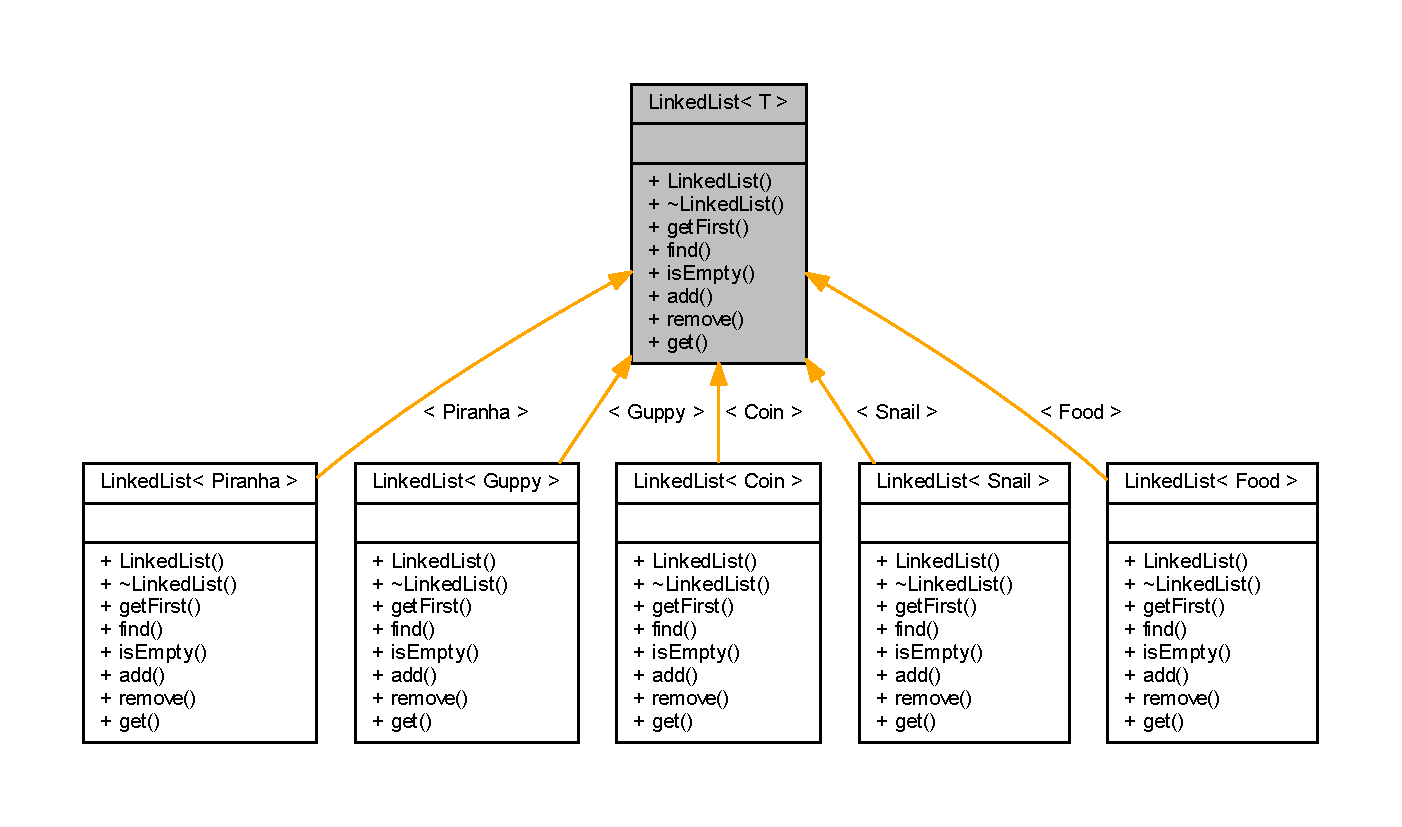
\includegraphics[width=350pt]{class_linked_list__inherit__graph}
\end{center}
\end{figure}


Collaboration diagram for Linked\+List$<$ T $>$\+:
\nopagebreak
\begin{figure}[H]
\begin{center}
\leavevmode
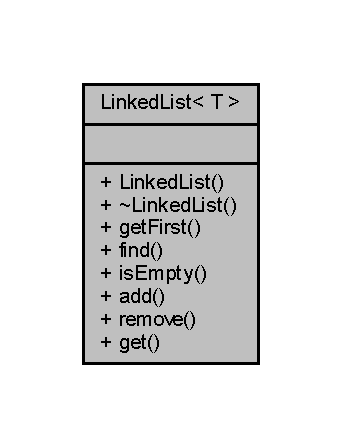
\includegraphics[width=164pt]{class_linked_list__coll__graph}
\end{center}
\end{figure}
\subsection*{Public Member Functions}
\begin{DoxyCompactItemize}
\item 
\mbox{\hyperlink{class_linked_list_ae04bfb6ff80214a33132ba72ceb117aa}{Linked\+List}} ()
\item 
Element\+List$<$ T $>$ \mbox{\hyperlink{class_linked_list_a312a0b29e235fdd9e0ceb42048e26600}{get\+First}} ()
\item 
int \mbox{\hyperlink{class_linked_list_abb5fc485a297b815daf6034f1c455979}{find}} (T element)
\item 
boolean \mbox{\hyperlink{class_linked_list_aecae3d82587c52087a4f65d6c56900e2}{is\+Empty}} ()
\item 
void \mbox{\hyperlink{class_linked_list_af7ec408e2f1040643d77f614af535988}{add}} (T element)
\item 
void \mbox{\hyperlink{class_linked_list_a85388ca2d7e4c8bc06fbea2c6fcfea33}{remove}} (T element)
\item 
T \mbox{\hyperlink{class_linked_list_a032ef46fc54f12525746d9f7c3a80663}{get}} (int index)
\end{DoxyCompactItemize}


\subsection{Constructor \& Destructor Documentation}
\mbox{\Hypertarget{class_linked_list_ae04bfb6ff80214a33132ba72ceb117aa}\label{class_linked_list_ae04bfb6ff80214a33132ba72ceb117aa}} 
\index{Linked\+List@{Linked\+List}!Linked\+List@{Linked\+List}}
\index{Linked\+List@{Linked\+List}!Linked\+List@{Linked\+List}}
\subsubsection{\texorpdfstring{Linked\+List()}{LinkedList()}}
{\footnotesize\ttfamily \mbox{\hyperlink{class_linked_list}{Linked\+List}}$<$ T $>$.\mbox{\hyperlink{class_linked_list}{Linked\+List}} (\begin{DoxyParamCaption}{ }\end{DoxyParamCaption})\hspace{0.3cm}{\ttfamily [inline]}}

Constructor \+: Initialize first with null 

\subsection{Member Function Documentation}
\mbox{\Hypertarget{class_linked_list_af7ec408e2f1040643d77f614af535988}\label{class_linked_list_af7ec408e2f1040643d77f614af535988}} 
\index{Linked\+List@{Linked\+List}!add@{add}}
\index{add@{add}!Linked\+List@{Linked\+List}}
\subsubsection{\texorpdfstring{add()}{add()}}
{\footnotesize\ttfamily void \mbox{\hyperlink{class_linked_list}{Linked\+List}}$<$ T $>$.add (\begin{DoxyParamCaption}\item[{T}]{element }\end{DoxyParamCaption})\hspace{0.3cm}{\ttfamily [inline]}}

Add element to the list 
\begin{DoxyParams}{Parameters}
{\em element} & element which will be added to list \\
\hline
\end{DoxyParams}
\mbox{\Hypertarget{class_linked_list_abb5fc485a297b815daf6034f1c455979}\label{class_linked_list_abb5fc485a297b815daf6034f1c455979}} 
\index{Linked\+List@{Linked\+List}!find@{find}}
\index{find@{find}!Linked\+List@{Linked\+List}}
\subsubsection{\texorpdfstring{find()}{find()}}
{\footnotesize\ttfamily int \mbox{\hyperlink{class_linked_list}{Linked\+List}}$<$ T $>$.find (\begin{DoxyParamCaption}\item[{T}]{element }\end{DoxyParamCaption})\hspace{0.3cm}{\ttfamily [inline]}}

Get index with value equals to argument. If not value found in list, then return -\/1 
\begin{DoxyParams}{Parameters}
{\em element} & data will be compared with this object \\
\hline
\end{DoxyParams}
\begin{DoxyReturn}{Returns}
index of element if found and -\/1 if not found 
\end{DoxyReturn}
\mbox{\Hypertarget{class_linked_list_a032ef46fc54f12525746d9f7c3a80663}\label{class_linked_list_a032ef46fc54f12525746d9f7c3a80663}} 
\index{Linked\+List@{Linked\+List}!get@{get}}
\index{get@{get}!Linked\+List@{Linked\+List}}
\subsubsection{\texorpdfstring{get()}{get()}}
{\footnotesize\ttfamily T \mbox{\hyperlink{class_linked_list}{Linked\+List}}$<$ T $>$.get (\begin{DoxyParamCaption}\item[{int}]{index }\end{DoxyParamCaption})\hspace{0.3cm}{\ttfamily [inline]}}

If found, return data of element list 
\begin{DoxyParams}{Parameters}
{\em index} & index of data which will be returned \\
\hline
\end{DoxyParams}
\begin{DoxyReturn}{Returns}
if found, return data of element list 
\end{DoxyReturn}
\mbox{\Hypertarget{class_linked_list_a312a0b29e235fdd9e0ceb42048e26600}\label{class_linked_list_a312a0b29e235fdd9e0ceb42048e26600}} 
\index{Linked\+List@{Linked\+List}!get\+First@{get\+First}}
\index{get\+First@{get\+First}!Linked\+List@{Linked\+List}}
\subsubsection{\texorpdfstring{get\+First()}{getFirst()}}
{\footnotesize\ttfamily Element\+List$<$T$>$ \mbox{\hyperlink{class_linked_list}{Linked\+List}}$<$ T $>$.get\+First (\begin{DoxyParamCaption}{ }\end{DoxyParamCaption})\hspace{0.3cm}{\ttfamily [inline]}}

Get variable first\textquotesingle{}s data \begin{DoxyReturn}{Returns}
variable first 
\end{DoxyReturn}
\mbox{\Hypertarget{class_linked_list_aecae3d82587c52087a4f65d6c56900e2}\label{class_linked_list_aecae3d82587c52087a4f65d6c56900e2}} 
\index{Linked\+List@{Linked\+List}!is\+Empty@{is\+Empty}}
\index{is\+Empty@{is\+Empty}!Linked\+List@{Linked\+List}}
\subsubsection{\texorpdfstring{is\+Empty()}{isEmpty()}}
{\footnotesize\ttfamily boolean \mbox{\hyperlink{class_linked_list}{Linked\+List}}$<$ T $>$.is\+Empty (\begin{DoxyParamCaption}{ }\end{DoxyParamCaption})\hspace{0.3cm}{\ttfamily [inline]}}

Return true if list is empty \begin{DoxyReturn}{Returns}
true if list is empty 
\end{DoxyReturn}
\mbox{\Hypertarget{class_linked_list_a85388ca2d7e4c8bc06fbea2c6fcfea33}\label{class_linked_list_a85388ca2d7e4c8bc06fbea2c6fcfea33}} 
\index{Linked\+List@{Linked\+List}!remove@{remove}}
\index{remove@{remove}!Linked\+List@{Linked\+List}}
\subsubsection{\texorpdfstring{remove()}{remove()}}
{\footnotesize\ttfamily void \mbox{\hyperlink{class_linked_list}{Linked\+List}}$<$ T $>$.remove (\begin{DoxyParamCaption}\item[{T}]{element }\end{DoxyParamCaption})\hspace{0.3cm}{\ttfamily [inline]}}

Remove first element in the list with same value as element 
\begin{DoxyParams}{Parameters}
{\em element} & value of element which will be removed \\
\hline
\end{DoxyParams}


The documentation for this class was generated from the following file\+:\begin{DoxyCompactItemize}
\item 
\mbox{\hyperlink{_linked_list_8java}{Linked\+List.\+java}}\end{DoxyCompactItemize}

\hypertarget{class_piranha}{}\section{Piranha Class Reference}
\label{class_piranha}\index{Piranha@{Piranha}}


{\ttfamily \#include $<$Piranha.\+hpp$>$}



Inheritance diagram for Piranha\+:
\nopagebreak
\begin{figure}[H]
\begin{center}
\leavevmode
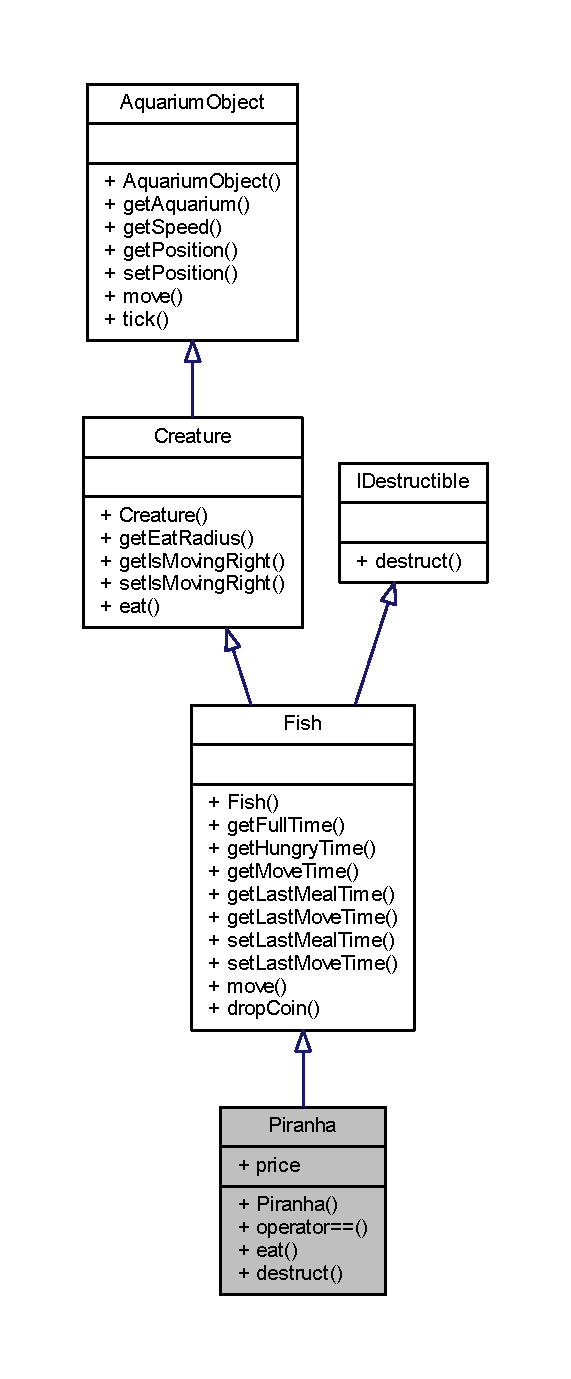
\includegraphics[height=550pt]{class_piranha__inherit__graph}
\end{center}
\end{figure}


Collaboration diagram for Piranha\+:
\nopagebreak
\begin{figure}[H]
\begin{center}
\leavevmode
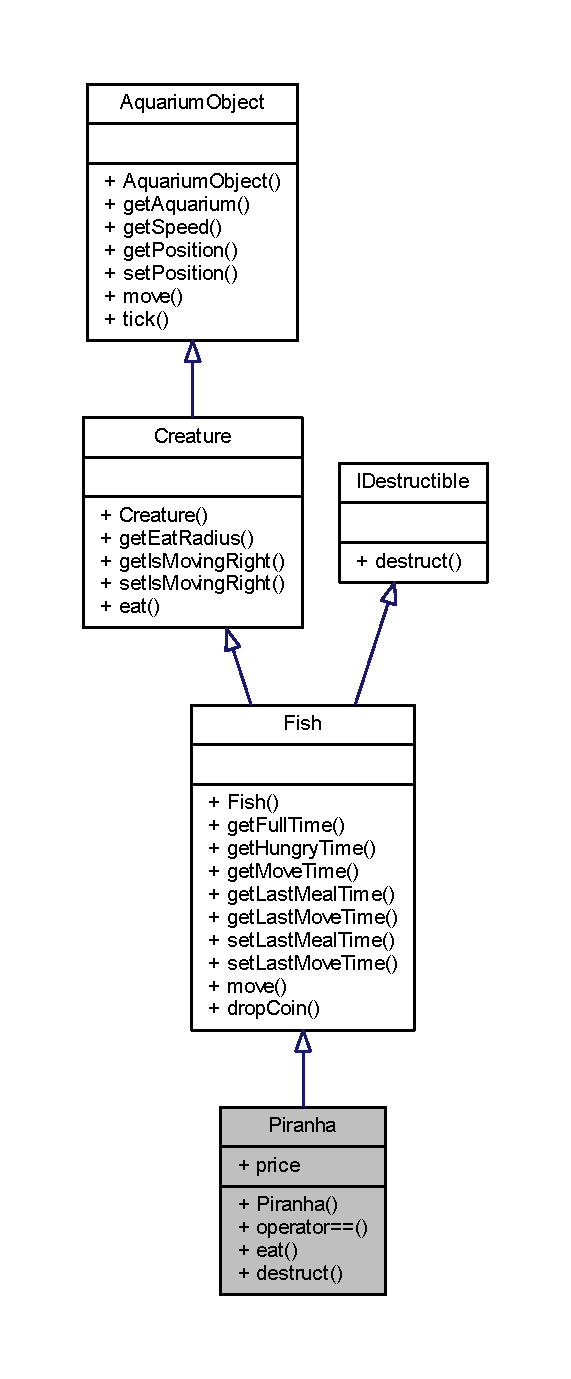
\includegraphics[height=550pt]{class_piranha__coll__graph}
\end{center}
\end{figure}
\subsection*{Public Member Functions}
\begin{DoxyCompactItemize}
\item 
\mbox{\hyperlink{class_piranha_a879b041f0a4bef2e837ee6dab37f7bc8}{Piranha}} (\mbox{\hyperlink{class_aquarium}{Aquarium}} \&\+\_\+aquarium)
\begin{DoxyCompactList}\small\item\em Constructor\+: instantiate piranha at speed of 7 and eat\+Radius of 75. \end{DoxyCompactList}\item 
bool \mbox{\hyperlink{class_piranha_ad374828e737e57a663689f5d54c9cf14}{operator==}} (const \mbox{\hyperlink{class_piranha}{Piranha}} \&other) const
\begin{DoxyCompactList}\small\item\em Reference comparison. \end{DoxyCompactList}\item 
\mbox{\hyperlink{struct_vector2}{Vector2}} \mbox{\hyperlink{class_piranha_a125847235bdbd0e8c676dcada0d86c14}{eat}} ()
\begin{DoxyCompactList}\small\item\em Find guppies in the aquarium. \end{DoxyCompactList}\item 
void \mbox{\hyperlink{class_piranha_a79c586a13bed4fb4aaa1b99c41c93c5a}{destruct}} ()
\begin{DoxyCompactList}\small\item\em Remove this piranha from aquarium. \end{DoxyCompactList}\end{DoxyCompactItemize}
\subsection*{Static Public Attributes}
\begin{DoxyCompactItemize}
\item 
static const int \mbox{\hyperlink{class_piranha_a5cab361b7ab7133245dc8a54a1d8addb}{price}} = 20
\end{DoxyCompactItemize}


\subsection{Constructor \& Destructor Documentation}
\mbox{\Hypertarget{class_piranha_a879b041f0a4bef2e837ee6dab37f7bc8}\label{class_piranha_a879b041f0a4bef2e837ee6dab37f7bc8}} 
\index{Piranha@{Piranha}!Piranha@{Piranha}}
\index{Piranha@{Piranha}!Piranha@{Piranha}}
\subsubsection{\texorpdfstring{Piranha()}{Piranha()}}
{\footnotesize\ttfamily Piranha\+::\+Piranha (\begin{DoxyParamCaption}\item[{\mbox{\hyperlink{class_aquarium}{Aquarium}} \&}]{\+\_\+aquarium }\end{DoxyParamCaption})}



Constructor\+: instantiate piranha at speed of 7 and eat\+Radius of 75. 



\subsection{Member Function Documentation}
\mbox{\Hypertarget{class_piranha_a79c586a13bed4fb4aaa1b99c41c93c5a}\label{class_piranha_a79c586a13bed4fb4aaa1b99c41c93c5a}} 
\index{Piranha@{Piranha}!destruct@{destruct}}
\index{destruct@{destruct}!Piranha@{Piranha}}
\subsubsection{\texorpdfstring{destruct()}{destruct()}}
{\footnotesize\ttfamily void Piranha\+::destruct (\begin{DoxyParamCaption}{ }\end{DoxyParamCaption})\hspace{0.3cm}{\ttfamily [virtual]}}



Remove this piranha from aquarium. 



Implements \mbox{\hyperlink{class_i_destructible_a63016d1bb4daa0a726fc8add9a0be62d}{I\+Destructible}}.

\mbox{\Hypertarget{class_piranha_a125847235bdbd0e8c676dcada0d86c14}\label{class_piranha_a125847235bdbd0e8c676dcada0d86c14}} 
\index{Piranha@{Piranha}!eat@{eat}}
\index{eat@{eat}!Piranha@{Piranha}}
\subsubsection{\texorpdfstring{eat()}{eat()}}
{\footnotesize\ttfamily \mbox{\hyperlink{struct_vector2}{Vector2}} Piranha\+::eat (\begin{DoxyParamCaption}{ }\end{DoxyParamCaption})\hspace{0.3cm}{\ttfamily [virtual]}}



Find guppies in the aquarium. 



Implements \mbox{\hyperlink{class_creature_a0d531a4c04c1021833ddb0e48864dbf4}{Creature}}.

\mbox{\Hypertarget{class_piranha_ad374828e737e57a663689f5d54c9cf14}\label{class_piranha_ad374828e737e57a663689f5d54c9cf14}} 
\index{Piranha@{Piranha}!operator==@{operator==}}
\index{operator==@{operator==}!Piranha@{Piranha}}
\subsubsection{\texorpdfstring{operator==()}{operator==()}}
{\footnotesize\ttfamily bool Piranha\+::operator== (\begin{DoxyParamCaption}\item[{const \mbox{\hyperlink{class_piranha}{Piranha}} \&}]{other }\end{DoxyParamCaption}) const}



Reference comparison. 



\subsection{Member Data Documentation}
\mbox{\Hypertarget{class_piranha_a5cab361b7ab7133245dc8a54a1d8addb}\label{class_piranha_a5cab361b7ab7133245dc8a54a1d8addb}} 
\index{Piranha@{Piranha}!price@{price}}
\index{price@{price}!Piranha@{Piranha}}
\subsubsection{\texorpdfstring{price}{price}}
{\footnotesize\ttfamily const int Piranha\+::price = 20\hspace{0.3cm}{\ttfamily [static]}}



The documentation for this class was generated from the following files\+:\begin{DoxyCompactItemize}
\item 
\mbox{\hyperlink{_piranha_8hpp}{Piranha.\+hpp}}\item 
\mbox{\hyperlink{_piranha_8cpp}{Piranha.\+cpp}}\end{DoxyCompactItemize}

\hypertarget{class_snail}{}\section{Snail Class Reference}
\label{class_snail}\index{Snail@{Snail}}


{\ttfamily \#include $<$Snail.\+hpp$>$}



Inheritance diagram for Snail\+:
% FIG 0


Collaboration diagram for Snail\+:
% FIG 1
\subsection*{Public Member Functions}
\begin{DoxyCompactItemize}
\item 
\mbox{\hyperlink{class_snail_acda391321646989553f4547dd793fa9c}{Snail}} (\mbox{\hyperlink{class_aquarium}{Aquarium}} \&\+\_\+aquarium)
\item 
bool \mbox{\hyperlink{class_snail_ab01308256de08e789ca752e1608120f7}{operator==}} (const \mbox{\hyperlink{class_snail}{Snail}} \&other) const
\item 
void \mbox{\hyperlink{class_snail_af5892ec122d9199480c813b74488256b}{move}} ()
\item 
\mbox{\hyperlink{struct_vector2}{Vector2}} \mbox{\hyperlink{class_snail_a0905a469c6333970b8246abca37795f1}{eat}} ()
\end{DoxyCompactItemize}


\subsection{Constructor \& Destructor Documentation}
\mbox{\Hypertarget{class_snail_acda391321646989553f4547dd793fa9c}\label{class_snail_acda391321646989553f4547dd793fa9c}} 
\index{Snail@{Snail}!Snail@{Snail}}
\index{Snail@{Snail}!Snail@{Snail}}
\subsubsection{\texorpdfstring{Snail()}{Snail()}}
{\footnotesize\ttfamily Snail\+::\+Snail (\begin{DoxyParamCaption}\item[{\mbox{\hyperlink{class_aquarium}{Aquarium}} \&}]{\+\_\+aquarium }\end{DoxyParamCaption})}



\subsection{Member Function Documentation}
\mbox{\Hypertarget{class_snail_a0905a469c6333970b8246abca37795f1}\label{class_snail_a0905a469c6333970b8246abca37795f1}} 
\index{Snail@{Snail}!eat@{eat}}
\index{eat@{eat}!Snail@{Snail}}
\subsubsection{\texorpdfstring{eat()}{eat()}}
{\footnotesize\ttfamily \mbox{\hyperlink{struct_vector2}{Vector2}} Snail\+::eat (\begin{DoxyParamCaption}{ }\end{DoxyParamCaption})\hspace{0.3cm}{\ttfamily [virtual]}}



Implements \mbox{\hyperlink{class_creature_a0d531a4c04c1021833ddb0e48864dbf4}{Creature}}.

\mbox{\Hypertarget{class_snail_af5892ec122d9199480c813b74488256b}\label{class_snail_af5892ec122d9199480c813b74488256b}} 
\index{Snail@{Snail}!move@{move}}
\index{move@{move}!Snail@{Snail}}
\subsubsection{\texorpdfstring{move()}{move()}}
{\footnotesize\ttfamily void Snail\+::move (\begin{DoxyParamCaption}{ }\end{DoxyParamCaption})\hspace{0.3cm}{\ttfamily [virtual]}}



Implements \mbox{\hyperlink{class_aquarium_object_a42c4de640f89ac8aebc26b7618578575}{Aquarium\+Object}}.

\mbox{\Hypertarget{class_snail_ab01308256de08e789ca752e1608120f7}\label{class_snail_ab01308256de08e789ca752e1608120f7}} 
\index{Snail@{Snail}!operator==@{operator==}}
\index{operator==@{operator==}!Snail@{Snail}}
\subsubsection{\texorpdfstring{operator==()}{operator==()}}
{\footnotesize\ttfamily bool Snail\+::operator== (\begin{DoxyParamCaption}\item[{const \mbox{\hyperlink{class_snail}{Snail}} \&}]{other }\end{DoxyParamCaption}) const}



The documentation for this class was generated from the following files\+:\begin{DoxyCompactItemize}
\item 
\mbox{\hyperlink{_snail_8hpp}{Snail.\+hpp}}\item 
\mbox{\hyperlink{_snail_8cpp}{Snail.\+cpp}}\end{DoxyCompactItemize}

\hypertarget{struct_vector2}{}\section{Vector2 Struct Reference}
\label{struct_vector2}\index{Vector2@{Vector2}}


{\ttfamily \#include $<$Vector2.\+hpp$>$}



Collaboration diagram for Vector2\+:
\nopagebreak
\begin{figure}[H]
\begin{center}
\leavevmode
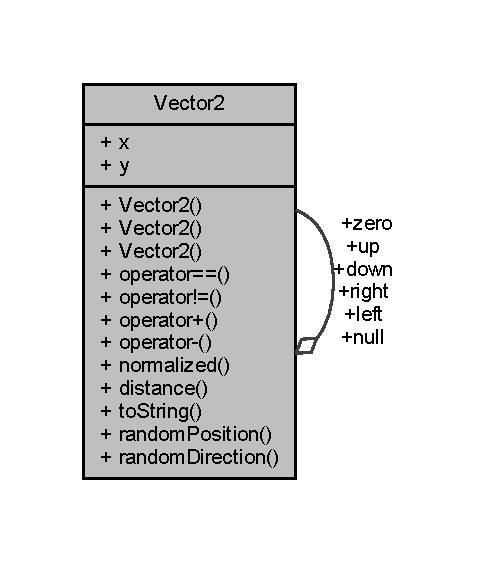
\includegraphics[width=229pt]{struct_vector2__coll__graph}
\end{center}
\end{figure}
\subsection*{Public Member Functions}
\begin{DoxyCompactItemize}
\item 
\mbox{\hyperlink{struct_vector2_a22104d1809be26a419ef1f959e3761bf}{Vector2}} ()
\begin{DoxyCompactList}\small\item\em Default constructor. \end{DoxyCompactList}\item 
\mbox{\hyperlink{struct_vector2_a861062b13bd0e92d50b3ffd90c9edd77}{Vector2}} (double \+\_\+x, double \+\_\+y)
\begin{DoxyCompactList}\small\item\em Constructor\+: x = \+\_\+x, y = \+\_\+y. \end{DoxyCompactList}\item 
\mbox{\hyperlink{struct_vector2_ac0c70e89b089fb619dae62c32ccde4ec}{Vector2}} (const \mbox{\hyperlink{struct_vector2}{Vector2}} \&other)
\begin{DoxyCompactList}\small\item\em Copy Constructor. \end{DoxyCompactList}\item 
bool \mbox{\hyperlink{struct_vector2_a75c903883dd1c8c6e39f83b3c0f1c6ab}{operator==}} (const \mbox{\hyperlink{struct_vector2}{Vector2}} \&other) const
\begin{DoxyCompactList}\small\item\em Equality operator. \end{DoxyCompactList}\item 
bool \mbox{\hyperlink{struct_vector2_af3b049c981a79bd60495b6362aa6392b}{operator!=}} (const \mbox{\hyperlink{struct_vector2}{Vector2}} \&other) const
\begin{DoxyCompactList}\small\item\em Inequality operator. \end{DoxyCompactList}\item 
\mbox{\hyperlink{struct_vector2}{Vector2}} \mbox{\hyperlink{struct_vector2_a53bdaa4ea8e1504f8a78ac78e6f151bf}{operator+}} (const \mbox{\hyperlink{struct_vector2}{Vector2}} \&other) const
\begin{DoxyCompactList}\small\item\em Addition. \end{DoxyCompactList}\item 
\mbox{\hyperlink{struct_vector2}{Vector2}} \mbox{\hyperlink{struct_vector2_a9f6650ee1529209532c14fc0e4e97a6a}{operator-\/}} (const \mbox{\hyperlink{struct_vector2}{Vector2}} \&other) const
\begin{DoxyCompactList}\small\item\em Substraction. \end{DoxyCompactList}\item 
\mbox{\hyperlink{struct_vector2}{Vector2}} \mbox{\hyperlink{struct_vector2_a1e0be0f2d578e8b5d0b8f95a9f8b6626}{normalized}} () const
\begin{DoxyCompactList}\small\item\em Return this vector2 with magnitude of 1. \end{DoxyCompactList}\item 
double \mbox{\hyperlink{struct_vector2_a75a29091c7c6f2f38e987ed2c62283c8}{distance}} (const \mbox{\hyperlink{struct_vector2}{Vector2}} \&other) const
\begin{DoxyCompactList}\small\item\em Return this vector2 distance to other vector2. \end{DoxyCompactList}\item 
std\+::string \mbox{\hyperlink{struct_vector2_abcf7d729573613553822f965c3b9a3d2}{to\+String}} ()
\end{DoxyCompactItemize}
\subsection*{Static Public Member Functions}
\begin{DoxyCompactItemize}
\item 
static \mbox{\hyperlink{struct_vector2}{Vector2}} \mbox{\hyperlink{struct_vector2_a13b12c4d8b92bbc3de6fca42cb7a2749}{random\+Position}} (double \mbox{\hyperlink{struct_vector2_a61d73d9036ccbb3257fbe595c014a1d0}{x}}, double \mbox{\hyperlink{struct_vector2_a4df9b2a8e79e6e30a7a3b34722d8b8b8}{y}})
\item 
static \mbox{\hyperlink{struct_vector2}{Vector2}} \mbox{\hyperlink{struct_vector2_a4ae4f36c515bda9939cfe36e58b25f45}{random\+Direction}} ()
\end{DoxyCompactItemize}
\subsection*{Public Attributes}
\begin{DoxyCompactItemize}
\item 
double \mbox{\hyperlink{struct_vector2_a61d73d9036ccbb3257fbe595c014a1d0}{x}}
\item 
double \mbox{\hyperlink{struct_vector2_a4df9b2a8e79e6e30a7a3b34722d8b8b8}{y}}
\end{DoxyCompactItemize}
\subsection*{Static Public Attributes}
\begin{DoxyCompactItemize}
\item 
static const \mbox{\hyperlink{struct_vector2}{Vector2}} \mbox{\hyperlink{struct_vector2_a2c6e0149051082f87c4f63f97e07c7ae}{null}} = \mbox{\hyperlink{struct_vector2}{Vector2}}(-\/1, -\/1)
\item 
static const \mbox{\hyperlink{struct_vector2}{Vector2}} \mbox{\hyperlink{struct_vector2_a28849e17f54c1c995f035544b5fd0a5f}{zero}} = \mbox{\hyperlink{struct_vector2}{Vector2}}()
\item 
static const \mbox{\hyperlink{struct_vector2}{Vector2}} \mbox{\hyperlink{struct_vector2_aa9712253176cedb918592990df5ea611}{right}} = \mbox{\hyperlink{struct_vector2}{Vector2}}(1, 0)
\item 
static const \mbox{\hyperlink{struct_vector2}{Vector2}} \mbox{\hyperlink{struct_vector2_a0de964f9acb5cc8669d0b3b9f5b9d4eb}{up}} = \mbox{\hyperlink{struct_vector2}{Vector2}}(0, -\/1)
\item 
static const \mbox{\hyperlink{struct_vector2}{Vector2}} \mbox{\hyperlink{struct_vector2_aaad26bbee0364de1e6a8676215886a2f}{left}} = \mbox{\hyperlink{struct_vector2}{Vector2}}(-\/1, 0)
\item 
static const \mbox{\hyperlink{struct_vector2}{Vector2}} \mbox{\hyperlink{struct_vector2_a64cb9ddeb42abbcfa527c3e2660ffef9}{down}} = \mbox{\hyperlink{struct_vector2}{Vector2}}(0, 1)
\end{DoxyCompactItemize}
\subsection*{Friends}
\begin{DoxyCompactItemize}
\item 
\mbox{\hyperlink{struct_vector2}{Vector2}} \mbox{\hyperlink{struct_vector2_a489f5283f5f1dc905c57d0a40d98c1af}{operator$\ast$}} (\mbox{\hyperlink{struct_vector2}{Vector2}} vector2, double k)
\begin{DoxyCompactList}\small\item\em Friend\+: \mbox{\hyperlink{struct_vector2}{Vector2}} times Double. \end{DoxyCompactList}\item 
\mbox{\hyperlink{struct_vector2}{Vector2}} \mbox{\hyperlink{struct_vector2_a6ac6360b23e2a1457b794f0aefc18f3a}{operator$\ast$}} (double k, \mbox{\hyperlink{struct_vector2}{Vector2}} vector2)
\begin{DoxyCompactList}\small\item\em Friend\+: Double times \mbox{\hyperlink{struct_vector2}{Vector2}}. \end{DoxyCompactList}\end{DoxyCompactItemize}


\subsection{Constructor \& Destructor Documentation}
\mbox{\Hypertarget{struct_vector2_a22104d1809be26a419ef1f959e3761bf}\label{struct_vector2_a22104d1809be26a419ef1f959e3761bf}} 
\index{Vector2@{Vector2}!Vector2@{Vector2}}
\index{Vector2@{Vector2}!Vector2@{Vector2}}
\subsubsection{\texorpdfstring{Vector2()}{Vector2()}\hspace{0.1cm}{\footnotesize\ttfamily [1/3]}}
{\footnotesize\ttfamily Vector2\+::\+Vector2 (\begin{DoxyParamCaption}{ }\end{DoxyParamCaption})}



Default constructor. 

\mbox{\Hypertarget{struct_vector2_a861062b13bd0e92d50b3ffd90c9edd77}\label{struct_vector2_a861062b13bd0e92d50b3ffd90c9edd77}} 
\index{Vector2@{Vector2}!Vector2@{Vector2}}
\index{Vector2@{Vector2}!Vector2@{Vector2}}
\subsubsection{\texorpdfstring{Vector2()}{Vector2()}\hspace{0.1cm}{\footnotesize\ttfamily [2/3]}}
{\footnotesize\ttfamily Vector2\+::\+Vector2 (\begin{DoxyParamCaption}\item[{double}]{\+\_\+x,  }\item[{double}]{\+\_\+y }\end{DoxyParamCaption})}



Constructor\+: x = \+\_\+x, y = \+\_\+y. 

\mbox{\Hypertarget{struct_vector2_ac0c70e89b089fb619dae62c32ccde4ec}\label{struct_vector2_ac0c70e89b089fb619dae62c32ccde4ec}} 
\index{Vector2@{Vector2}!Vector2@{Vector2}}
\index{Vector2@{Vector2}!Vector2@{Vector2}}
\subsubsection{\texorpdfstring{Vector2()}{Vector2()}\hspace{0.1cm}{\footnotesize\ttfamily [3/3]}}
{\footnotesize\ttfamily Vector2\+::\+Vector2 (\begin{DoxyParamCaption}\item[{const \mbox{\hyperlink{struct_vector2}{Vector2}} \&}]{other }\end{DoxyParamCaption})}



Copy Constructor. 



\subsection{Member Function Documentation}
\mbox{\Hypertarget{struct_vector2_a75a29091c7c6f2f38e987ed2c62283c8}\label{struct_vector2_a75a29091c7c6f2f38e987ed2c62283c8}} 
\index{Vector2@{Vector2}!distance@{distance}}
\index{distance@{distance}!Vector2@{Vector2}}
\subsubsection{\texorpdfstring{distance()}{distance()}}
{\footnotesize\ttfamily double Vector2\+::distance (\begin{DoxyParamCaption}\item[{const \mbox{\hyperlink{struct_vector2}{Vector2}} \&}]{other }\end{DoxyParamCaption}) const}



Return this vector2 distance to other vector2. 

\mbox{\Hypertarget{struct_vector2_a1e0be0f2d578e8b5d0b8f95a9f8b6626}\label{struct_vector2_a1e0be0f2d578e8b5d0b8f95a9f8b6626}} 
\index{Vector2@{Vector2}!normalized@{normalized}}
\index{normalized@{normalized}!Vector2@{Vector2}}
\subsubsection{\texorpdfstring{normalized()}{normalized()}}
{\footnotesize\ttfamily \mbox{\hyperlink{struct_vector2}{Vector2}} Vector2\+::normalized (\begin{DoxyParamCaption}{ }\end{DoxyParamCaption}) const}



Return this vector2 with magnitude of 1. 

\mbox{\Hypertarget{struct_vector2_af3b049c981a79bd60495b6362aa6392b}\label{struct_vector2_af3b049c981a79bd60495b6362aa6392b}} 
\index{Vector2@{Vector2}!operator"!=@{operator"!=}}
\index{operator"!=@{operator"!=}!Vector2@{Vector2}}
\subsubsection{\texorpdfstring{operator"!=()}{operator!=()}}
{\footnotesize\ttfamily bool Vector2\+::operator!= (\begin{DoxyParamCaption}\item[{const \mbox{\hyperlink{struct_vector2}{Vector2}} \&}]{other }\end{DoxyParamCaption}) const}



Inequality operator. 

\mbox{\Hypertarget{struct_vector2_a53bdaa4ea8e1504f8a78ac78e6f151bf}\label{struct_vector2_a53bdaa4ea8e1504f8a78ac78e6f151bf}} 
\index{Vector2@{Vector2}!operator+@{operator+}}
\index{operator+@{operator+}!Vector2@{Vector2}}
\subsubsection{\texorpdfstring{operator+()}{operator+()}}
{\footnotesize\ttfamily \mbox{\hyperlink{struct_vector2}{Vector2}} Vector2\+::operator+ (\begin{DoxyParamCaption}\item[{const \mbox{\hyperlink{struct_vector2}{Vector2}} \&}]{other }\end{DoxyParamCaption}) const}



Addition. 

\mbox{\Hypertarget{struct_vector2_a9f6650ee1529209532c14fc0e4e97a6a}\label{struct_vector2_a9f6650ee1529209532c14fc0e4e97a6a}} 
\index{Vector2@{Vector2}!operator-\/@{operator-\/}}
\index{operator-\/@{operator-\/}!Vector2@{Vector2}}
\subsubsection{\texorpdfstring{operator-\/()}{operator-()}}
{\footnotesize\ttfamily \mbox{\hyperlink{struct_vector2}{Vector2}} Vector2\+::operator-\/ (\begin{DoxyParamCaption}\item[{const \mbox{\hyperlink{struct_vector2}{Vector2}} \&}]{other }\end{DoxyParamCaption}) const}



Substraction. 

\mbox{\Hypertarget{struct_vector2_a75c903883dd1c8c6e39f83b3c0f1c6ab}\label{struct_vector2_a75c903883dd1c8c6e39f83b3c0f1c6ab}} 
\index{Vector2@{Vector2}!operator==@{operator==}}
\index{operator==@{operator==}!Vector2@{Vector2}}
\subsubsection{\texorpdfstring{operator==()}{operator==()}}
{\footnotesize\ttfamily bool Vector2\+::operator== (\begin{DoxyParamCaption}\item[{const \mbox{\hyperlink{struct_vector2}{Vector2}} \&}]{other }\end{DoxyParamCaption}) const}



Equality operator. 

\mbox{\Hypertarget{struct_vector2_a4ae4f36c515bda9939cfe36e58b25f45}\label{struct_vector2_a4ae4f36c515bda9939cfe36e58b25f45}} 
\index{Vector2@{Vector2}!random\+Direction@{random\+Direction}}
\index{random\+Direction@{random\+Direction}!Vector2@{Vector2}}
\subsubsection{\texorpdfstring{random\+Direction()}{randomDirection()}}
{\footnotesize\ttfamily \mbox{\hyperlink{struct_vector2}{Vector2}} Vector2\+::random\+Direction (\begin{DoxyParamCaption}{ }\end{DoxyParamCaption})\hspace{0.3cm}{\ttfamily [static]}}

\mbox{\Hypertarget{struct_vector2_a13b12c4d8b92bbc3de6fca42cb7a2749}\label{struct_vector2_a13b12c4d8b92bbc3de6fca42cb7a2749}} 
\index{Vector2@{Vector2}!random\+Position@{random\+Position}}
\index{random\+Position@{random\+Position}!Vector2@{Vector2}}
\subsubsection{\texorpdfstring{random\+Position()}{randomPosition()}}
{\footnotesize\ttfamily \mbox{\hyperlink{struct_vector2}{Vector2}} Vector2\+::random\+Position (\begin{DoxyParamCaption}\item[{double}]{x,  }\item[{double}]{y }\end{DoxyParamCaption})\hspace{0.3cm}{\ttfamily [static]}}

\mbox{\Hypertarget{struct_vector2_abcf7d729573613553822f965c3b9a3d2}\label{struct_vector2_abcf7d729573613553822f965c3b9a3d2}} 
\index{Vector2@{Vector2}!to\+String@{to\+String}}
\index{to\+String@{to\+String}!Vector2@{Vector2}}
\subsubsection{\texorpdfstring{to\+String()}{toString()}}
{\footnotesize\ttfamily std\+::string Vector2\+::to\+String (\begin{DoxyParamCaption}{ }\end{DoxyParamCaption})}



\subsection{Friends And Related Function Documentation}
\mbox{\Hypertarget{struct_vector2_a489f5283f5f1dc905c57d0a40d98c1af}\label{struct_vector2_a489f5283f5f1dc905c57d0a40d98c1af}} 
\index{Vector2@{Vector2}!operator$\ast$@{operator$\ast$}}
\index{operator$\ast$@{operator$\ast$}!Vector2@{Vector2}}
\subsubsection{\texorpdfstring{operator$\ast$}{operator*}\hspace{0.1cm}{\footnotesize\ttfamily [1/2]}}
{\footnotesize\ttfamily \mbox{\hyperlink{struct_vector2}{Vector2}} operator$\ast$ (\begin{DoxyParamCaption}\item[{\mbox{\hyperlink{struct_vector2}{Vector2}}}]{vector2,  }\item[{double}]{k }\end{DoxyParamCaption})\hspace{0.3cm}{\ttfamily [friend]}}



Friend\+: \mbox{\hyperlink{struct_vector2}{Vector2}} times Double. 

\mbox{\Hypertarget{struct_vector2_a6ac6360b23e2a1457b794f0aefc18f3a}\label{struct_vector2_a6ac6360b23e2a1457b794f0aefc18f3a}} 
\index{Vector2@{Vector2}!operator$\ast$@{operator$\ast$}}
\index{operator$\ast$@{operator$\ast$}!Vector2@{Vector2}}
\subsubsection{\texorpdfstring{operator$\ast$}{operator*}\hspace{0.1cm}{\footnotesize\ttfamily [2/2]}}
{\footnotesize\ttfamily \mbox{\hyperlink{struct_vector2}{Vector2}} operator$\ast$ (\begin{DoxyParamCaption}\item[{double}]{k,  }\item[{\mbox{\hyperlink{struct_vector2}{Vector2}}}]{vector2 }\end{DoxyParamCaption})\hspace{0.3cm}{\ttfamily [friend]}}



Friend\+: Double times \mbox{\hyperlink{struct_vector2}{Vector2}}. 



\subsection{Member Data Documentation}
\mbox{\Hypertarget{struct_vector2_a64cb9ddeb42abbcfa527c3e2660ffef9}\label{struct_vector2_a64cb9ddeb42abbcfa527c3e2660ffef9}} 
\index{Vector2@{Vector2}!down@{down}}
\index{down@{down}!Vector2@{Vector2}}
\subsubsection{\texorpdfstring{down}{down}}
{\footnotesize\ttfamily const \mbox{\hyperlink{struct_vector2}{Vector2}} Vector2\+::down = \mbox{\hyperlink{struct_vector2}{Vector2}}(0, 1)\hspace{0.3cm}{\ttfamily [static]}}

\mbox{\Hypertarget{struct_vector2_aaad26bbee0364de1e6a8676215886a2f}\label{struct_vector2_aaad26bbee0364de1e6a8676215886a2f}} 
\index{Vector2@{Vector2}!left@{left}}
\index{left@{left}!Vector2@{Vector2}}
\subsubsection{\texorpdfstring{left}{left}}
{\footnotesize\ttfamily const \mbox{\hyperlink{struct_vector2}{Vector2}} Vector2\+::left = \mbox{\hyperlink{struct_vector2}{Vector2}}(-\/1, 0)\hspace{0.3cm}{\ttfamily [static]}}

\mbox{\Hypertarget{struct_vector2_a2c6e0149051082f87c4f63f97e07c7ae}\label{struct_vector2_a2c6e0149051082f87c4f63f97e07c7ae}} 
\index{Vector2@{Vector2}!null@{null}}
\index{null@{null}!Vector2@{Vector2}}
\subsubsection{\texorpdfstring{null}{null}}
{\footnotesize\ttfamily const \mbox{\hyperlink{struct_vector2}{Vector2}} Vector2\+::null = \mbox{\hyperlink{struct_vector2}{Vector2}}(-\/1, -\/1)\hspace{0.3cm}{\ttfamily [static]}}

\mbox{\Hypertarget{struct_vector2_aa9712253176cedb918592990df5ea611}\label{struct_vector2_aa9712253176cedb918592990df5ea611}} 
\index{Vector2@{Vector2}!right@{right}}
\index{right@{right}!Vector2@{Vector2}}
\subsubsection{\texorpdfstring{right}{right}}
{\footnotesize\ttfamily const \mbox{\hyperlink{struct_vector2}{Vector2}} Vector2\+::right = \mbox{\hyperlink{struct_vector2}{Vector2}}(1, 0)\hspace{0.3cm}{\ttfamily [static]}}

\mbox{\Hypertarget{struct_vector2_a0de964f9acb5cc8669d0b3b9f5b9d4eb}\label{struct_vector2_a0de964f9acb5cc8669d0b3b9f5b9d4eb}} 
\index{Vector2@{Vector2}!up@{up}}
\index{up@{up}!Vector2@{Vector2}}
\subsubsection{\texorpdfstring{up}{up}}
{\footnotesize\ttfamily const \mbox{\hyperlink{struct_vector2}{Vector2}} Vector2\+::up = \mbox{\hyperlink{struct_vector2}{Vector2}}(0, -\/1)\hspace{0.3cm}{\ttfamily [static]}}

\mbox{\Hypertarget{struct_vector2_a61d73d9036ccbb3257fbe595c014a1d0}\label{struct_vector2_a61d73d9036ccbb3257fbe595c014a1d0}} 
\index{Vector2@{Vector2}!x@{x}}
\index{x@{x}!Vector2@{Vector2}}
\subsubsection{\texorpdfstring{x}{x}}
{\footnotesize\ttfamily double Vector2\+::x}

\mbox{\Hypertarget{struct_vector2_a4df9b2a8e79e6e30a7a3b34722d8b8b8}\label{struct_vector2_a4df9b2a8e79e6e30a7a3b34722d8b8b8}} 
\index{Vector2@{Vector2}!y@{y}}
\index{y@{y}!Vector2@{Vector2}}
\subsubsection{\texorpdfstring{y}{y}}
{\footnotesize\ttfamily double Vector2\+::y}

\mbox{\Hypertarget{struct_vector2_a28849e17f54c1c995f035544b5fd0a5f}\label{struct_vector2_a28849e17f54c1c995f035544b5fd0a5f}} 
\index{Vector2@{Vector2}!zero@{zero}}
\index{zero@{zero}!Vector2@{Vector2}}
\subsubsection{\texorpdfstring{zero}{zero}}
{\footnotesize\ttfamily const \mbox{\hyperlink{struct_vector2}{Vector2}} Vector2\+::zero = \mbox{\hyperlink{struct_vector2}{Vector2}}()\hspace{0.3cm}{\ttfamily [static]}}



The documentation for this struct was generated from the following files\+:\begin{DoxyCompactItemize}
\item 
\mbox{\hyperlink{_vector2_8hpp}{Vector2.\+hpp}}\item 
\mbox{\hyperlink{_vector2_8cpp}{Vector2.\+cpp}}\end{DoxyCompactItemize}

\chapter{File Documentation}
\hypertarget{_aquarium_8cpp}{}\section{Aquarium.\+cpp File Reference}
\label{_aquarium_8cpp}\index{Aquarium.\+cpp@{Aquarium.\+cpp}}
{\ttfamily \#include \char`\"{}Aquarium.\+hpp\char`\"{}}\newline
Include dependency graph for Aquarium.\+cpp\+:

\hypertarget{_aquarium_8hpp}{}\section{Aquarium.\+hpp File Reference}
\label{_aquarium_8hpp}\index{Aquarium.\+hpp@{Aquarium.\+hpp}}
{\ttfamily \#include \char`\"{}Guppy.\+hpp\char`\"{}}\newline
{\ttfamily \#include \char`\"{}Piranha.\+hpp\char`\"{}}\newline
{\ttfamily \#include \char`\"{}Snail.\+hpp\char`\"{}}\newline
{\ttfamily \#include \char`\"{}Food.\+hpp\char`\"{}}\newline
{\ttfamily \#include \char`\"{}Coin.\+hpp\char`\"{}}\newline
{\ttfamily \#include \char`\"{}Linked\+List.\+hpp\char`\"{}}\newline
Include dependency graph for Aquarium.\+hpp\+:
\nopagebreak
\begin{figure}[H]
\begin{center}
\leavevmode
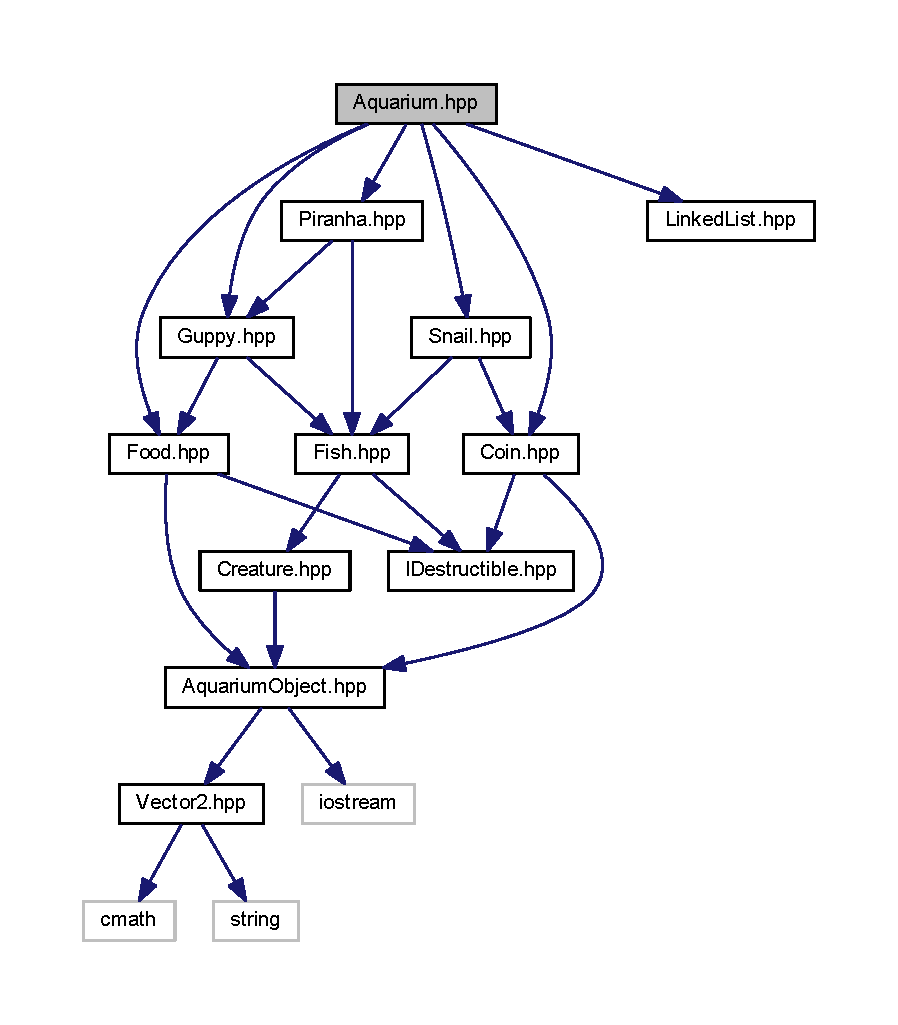
\includegraphics[width=350pt]{_aquarium_8hpp__incl}
\end{center}
\end{figure}
This graph shows which files directly or indirectly include this file\+:
\nopagebreak
\begin{figure}[H]
\begin{center}
\leavevmode
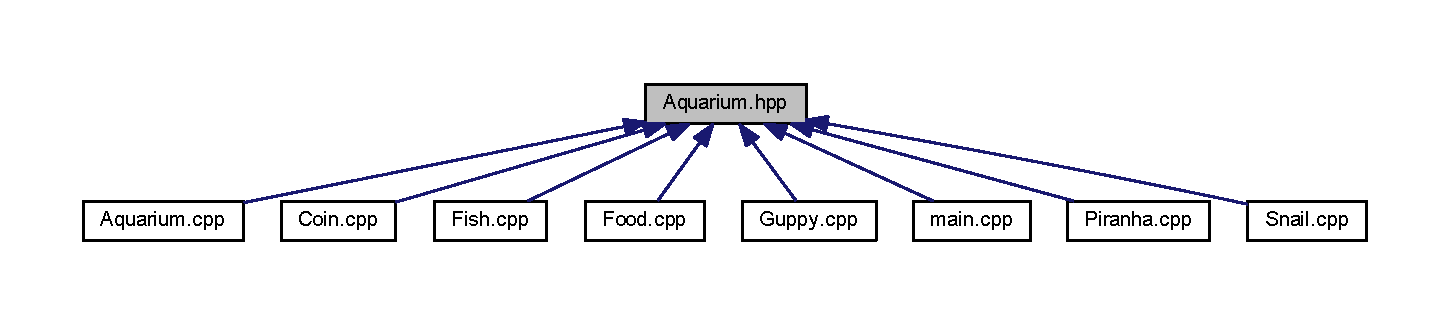
\includegraphics[width=350pt]{_aquarium_8hpp__dep__incl}
\end{center}
\end{figure}
\subsection*{Classes}
\begin{DoxyCompactItemize}
\item 
class \mbox{\hyperlink{class_aquarium}{Aquarium}}
\end{DoxyCompactItemize}

\hypertarget{_aquarium_object_8cpp}{}\section{Aquarium\+Object.\+cpp File Reference}
\label{_aquarium_object_8cpp}\index{Aquarium\+Object.\+cpp@{Aquarium\+Object.\+cpp}}
{\ttfamily \#include \char`\"{}Aquarium\+Object.\+hpp\char`\"{}}\newline
Include dependency graph for Aquarium\+Object.\+cpp\+:\nopagebreak
\begin{figure}[H]
\begin{center}
\leavevmode
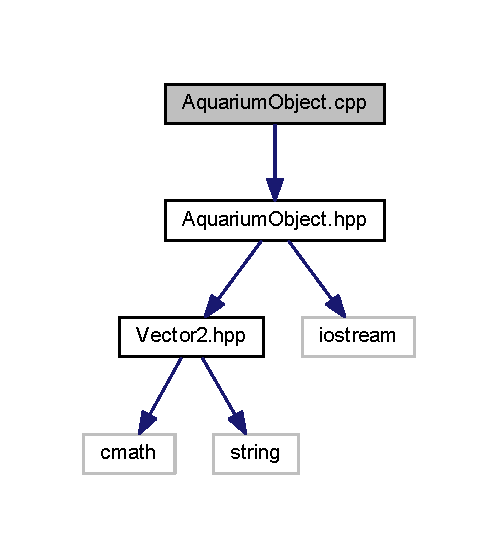
\includegraphics[width=239pt]{_aquarium_object_8cpp__incl}
\end{center}
\end{figure}

\hypertarget{_aquarium_object_8hpp}{}\section{Aquarium\+Object.\+hpp File Reference}
\label{_aquarium_object_8hpp}\index{Aquarium\+Object.\+hpp@{Aquarium\+Object.\+hpp}}
{\ttfamily \#include \char`\"{}Vector2.\+hpp\char`\"{}}\newline
{\ttfamily \#include $<$iostream$>$}\newline
Include dependency graph for Aquarium\+Object.\+hpp\+:\nopagebreak
\begin{figure}[H]
\begin{center}
\leavevmode
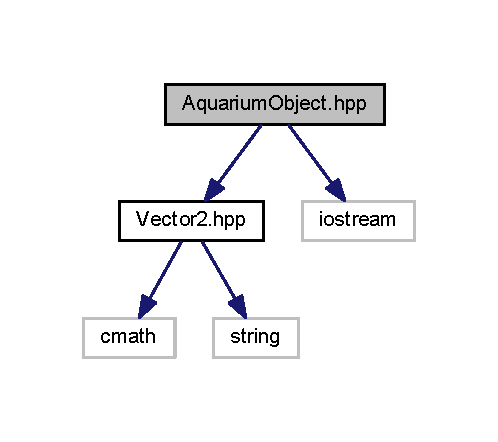
\includegraphics[width=239pt]{_aquarium_object_8hpp__incl}
\end{center}
\end{figure}
This graph shows which files directly or indirectly include this file\+:\nopagebreak
\begin{figure}[H]
\begin{center}
\leavevmode
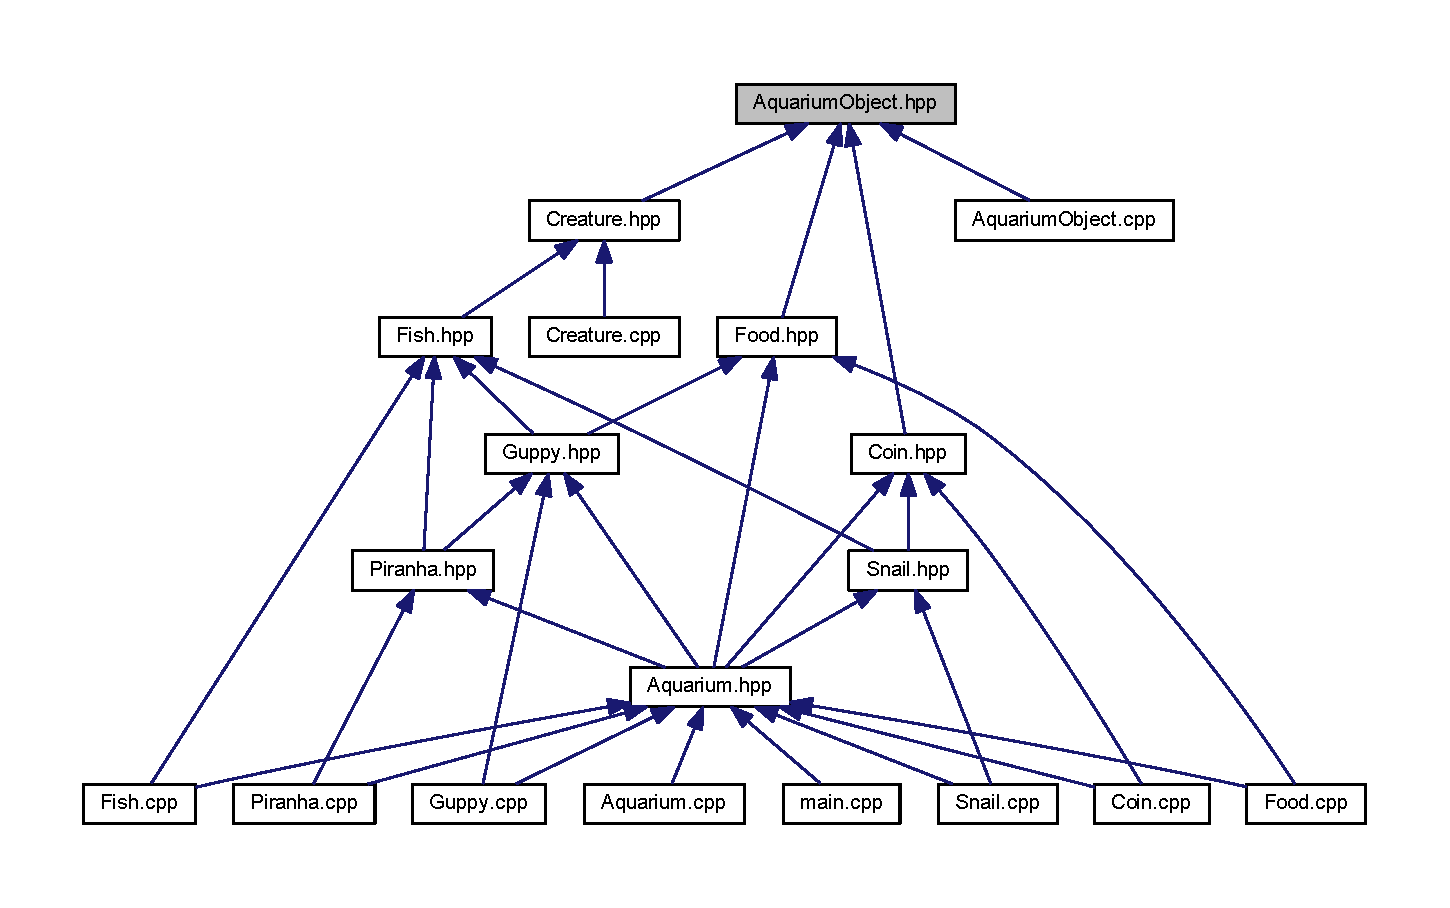
\includegraphics[width=350pt]{_aquarium_object_8hpp__dep__incl}
\end{center}
\end{figure}
\subsection*{Classes}
\begin{DoxyCompactItemize}
\item 
class \mbox{\hyperlink{class_aquarium_object}{Aquarium\+Object}}
\end{DoxyCompactItemize}

\hypertarget{_coin_8cpp}{}\section{Coin.\+cpp File Reference}
\label{_coin_8cpp}\index{Coin.\+cpp@{Coin.\+cpp}}
{\ttfamily \#include \char`\"{}Coin.\+hpp\char`\"{}}\newline
{\ttfamily \#include \char`\"{}Aquarium.\+hpp\char`\"{}}\newline
Include dependency graph for Coin.\+cpp\+:
% FIG 0

\hypertarget{_coin_8hpp}{}\section{Coin.\+hpp File Reference}
\label{_coin_8hpp}\index{Coin.\+hpp@{Coin.\+hpp}}
{\ttfamily \#include \char`\"{}Aquarium\+Object.\+hpp\char`\"{}}\newline
{\ttfamily \#include \char`\"{}I\+Destructible.\+hpp\char`\"{}}\newline
Include dependency graph for Coin.\+hpp\+:
% FIG 0
This graph shows which files directly or indirectly include this file\+:
% FIG 1
\subsection*{Classes}
\begin{DoxyCompactItemize}
\item 
class \mbox{\hyperlink{class_coin}{Coin}}
\end{DoxyCompactItemize}

\hypertarget{_creature_8cpp}{}\section{Creature.\+cpp File Reference}
\label{_creature_8cpp}\index{Creature.\+cpp@{Creature.\+cpp}}
{\ttfamily \#include \char`\"{}Creature.\+hpp\char`\"{}}\newline
Include dependency graph for Creature.\+cpp\+:\nopagebreak
\begin{figure}[H]
\begin{center}
\leavevmode
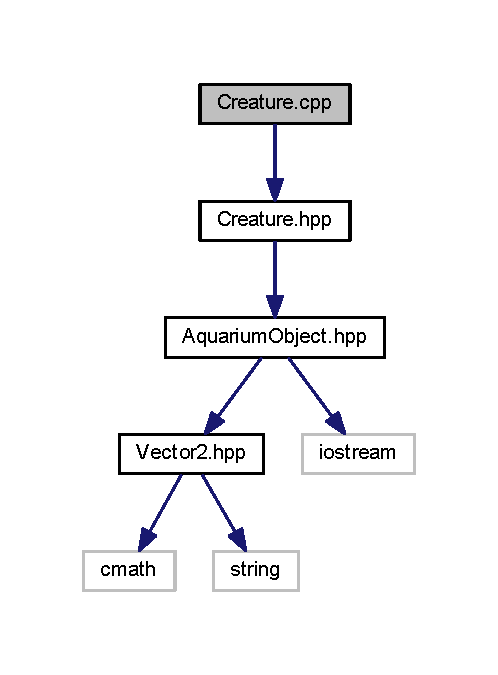
\includegraphics[width=239pt]{_creature_8cpp__incl}
\end{center}
\end{figure}

\hypertarget{_creature_8hpp}{}\section{Creature.\+hpp File Reference}
\label{_creature_8hpp}\index{Creature.\+hpp@{Creature.\+hpp}}
{\ttfamily \#include \char`\"{}Aquarium\+Object.\+hpp\char`\"{}}\newline
Include dependency graph for Creature.\+hpp\+:\nopagebreak
\begin{figure}[H]
\begin{center}
\leavevmode
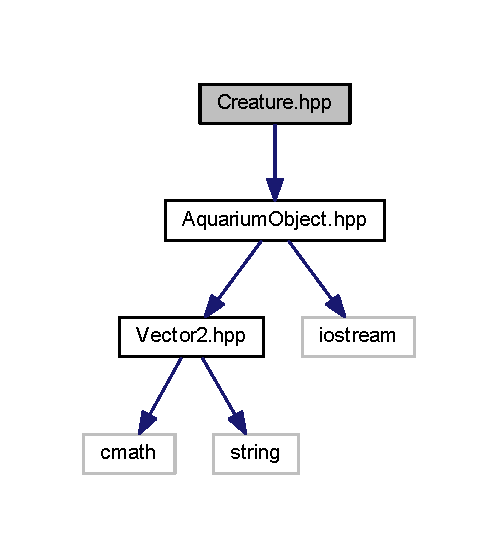
\includegraphics[width=239pt]{_creature_8hpp__incl}
\end{center}
\end{figure}
This graph shows which files directly or indirectly include this file\+:\nopagebreak
\begin{figure}[H]
\begin{center}
\leavevmode
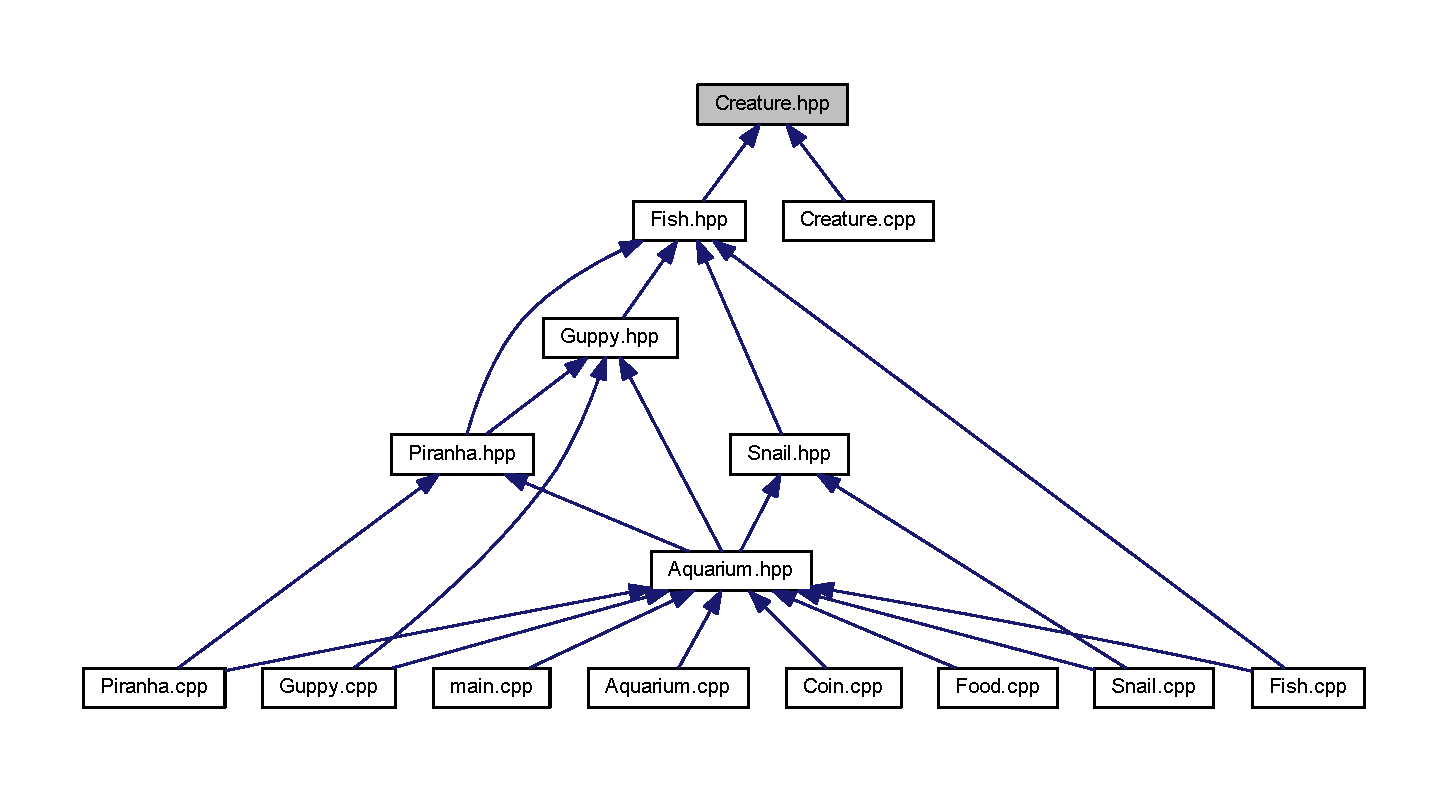
\includegraphics[width=350pt]{_creature_8hpp__dep__incl}
\end{center}
\end{figure}
\subsection*{Classes}
\begin{DoxyCompactItemize}
\item 
class \mbox{\hyperlink{class_creature}{Creature}}
\end{DoxyCompactItemize}

\hypertarget{_fish_8cpp}{}\section{Fish.\+cpp File Reference}
\label{_fish_8cpp}\index{Fish.\+cpp@{Fish.\+cpp}}
{\ttfamily \#include \char`\"{}Fish.\+hpp\char`\"{}}\newline
{\ttfamily \#include \char`\"{}Aquarium.\+hpp\char`\"{}}\newline
Include dependency graph for Fish.\+cpp\+:
\nopagebreak
\begin{figure}[H]
\begin{center}
\leavevmode
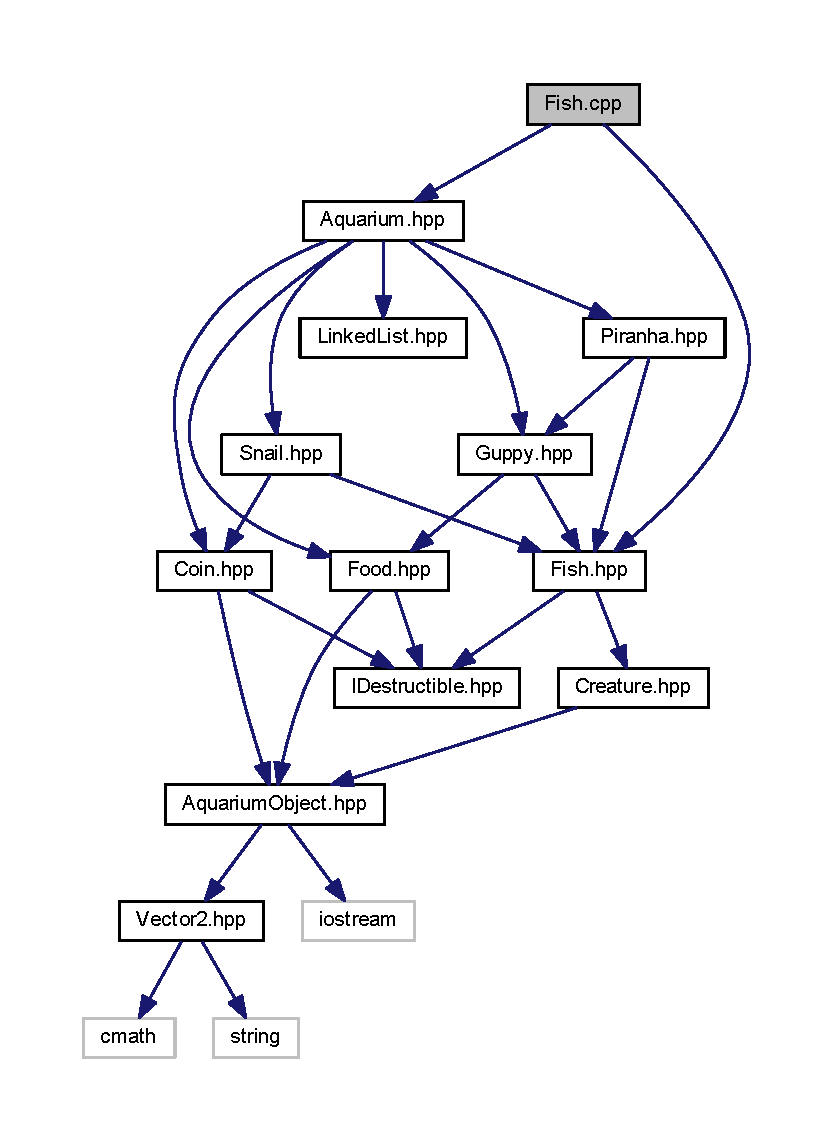
\includegraphics[width=350pt]{_fish_8cpp__incl}
\end{center}
\end{figure}

\hypertarget{_fish_8hpp}{}\section{Fish.\+hpp File Reference}
\label{_fish_8hpp}\index{Fish.\+hpp@{Fish.\+hpp}}
{\ttfamily \#include \char`\"{}Creature.\+hpp\char`\"{}}\newline
{\ttfamily \#include \char`\"{}I\+Destructible.\+hpp\char`\"{}}\newline
Include dependency graph for Fish.\+hpp\+:\nopagebreak
\begin{figure}[H]
\begin{center}
\leavevmode
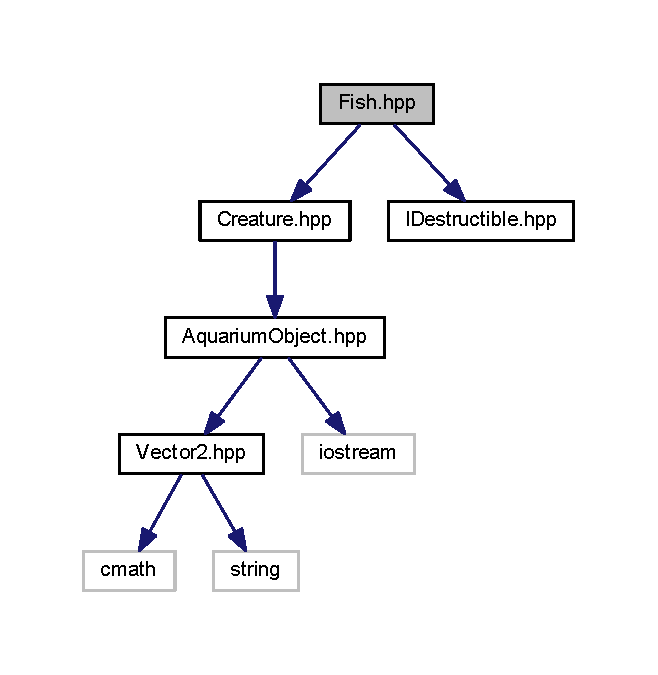
\includegraphics[width=316pt]{_fish_8hpp__incl}
\end{center}
\end{figure}
This graph shows which files directly or indirectly include this file\+:\nopagebreak
\begin{figure}[H]
\begin{center}
\leavevmode
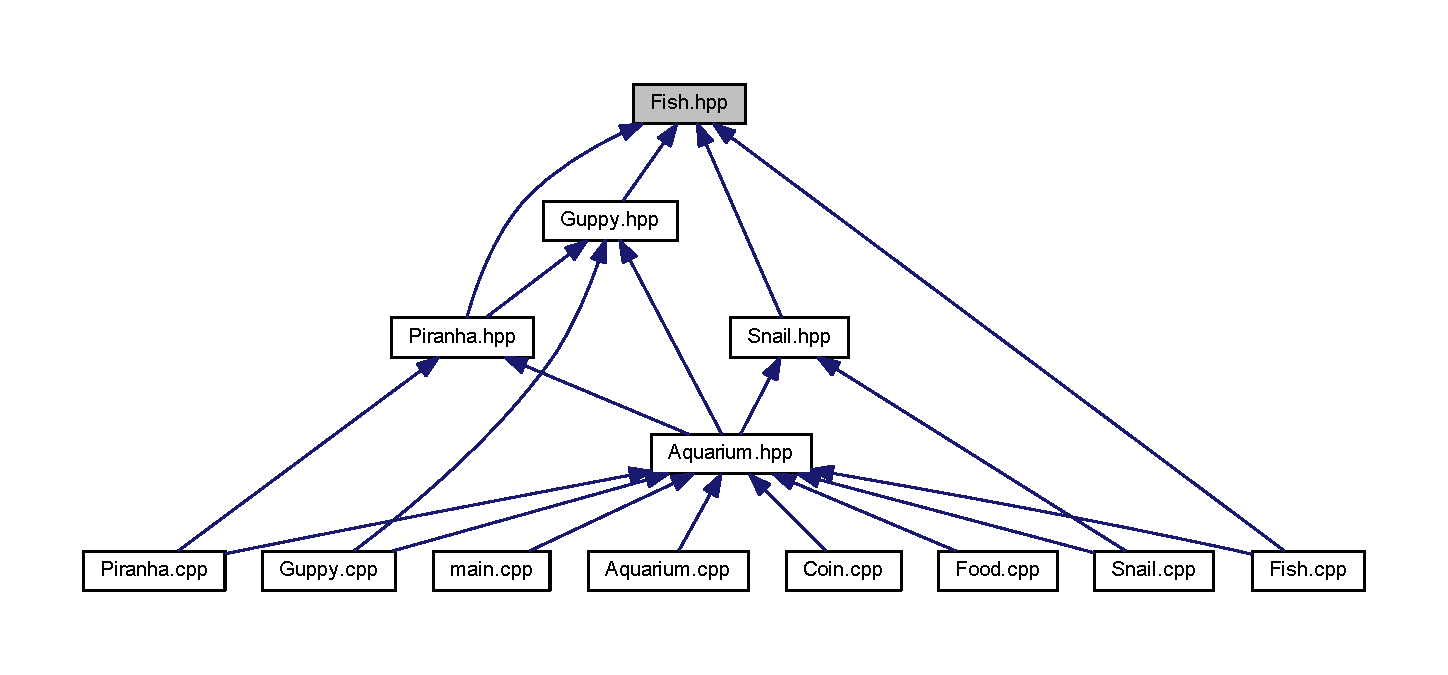
\includegraphics[width=350pt]{_fish_8hpp__dep__incl}
\end{center}
\end{figure}
\subsection*{Classes}
\begin{DoxyCompactItemize}
\item 
class \mbox{\hyperlink{class_fish}{Fish}}
\end{DoxyCompactItemize}

\hypertarget{_food_8cpp}{}\section{Food.\+cpp File Reference}
\label{_food_8cpp}\index{Food.\+cpp@{Food.\+cpp}}
{\ttfamily \#include \char`\"{}Food.\+hpp\char`\"{}}\newline
{\ttfamily \#include \char`\"{}Aquarium.\+hpp\char`\"{}}\newline
Include dependency graph for Food.\+cpp\+:
% FIG 0

\hypertarget{_food_8hpp}{}\section{Food.\+hpp File Reference}
\label{_food_8hpp}\index{Food.\+hpp@{Food.\+hpp}}
{\ttfamily \#include \char`\"{}Aquarium\+Object.\+hpp\char`\"{}}\newline
{\ttfamily \#include \char`\"{}I\+Destructible.\+hpp\char`\"{}}\newline
Include dependency graph for Food.\+hpp\+:
\nopagebreak
\begin{figure}[H]
\begin{center}
\leavevmode
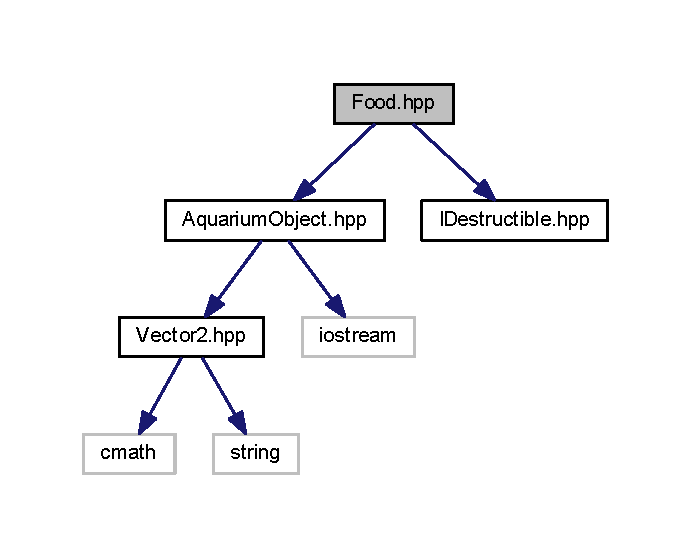
\includegraphics[width=332pt]{_food_8hpp__incl}
\end{center}
\end{figure}
This graph shows which files directly or indirectly include this file\+:
\nopagebreak
\begin{figure}[H]
\begin{center}
\leavevmode
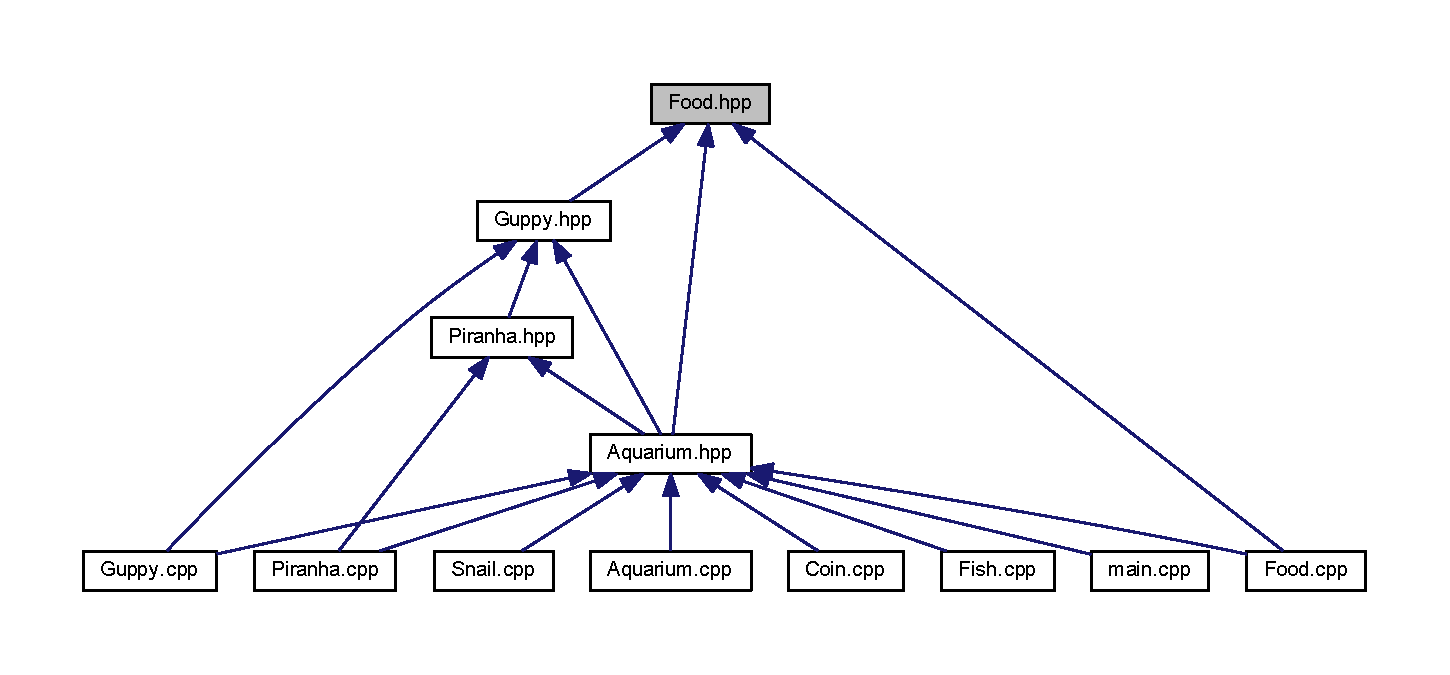
\includegraphics[width=350pt]{_food_8hpp__dep__incl}
\end{center}
\end{figure}
\subsection*{Classes}
\begin{DoxyCompactItemize}
\item 
class \mbox{\hyperlink{class_food}{Food}}
\end{DoxyCompactItemize}

\hypertarget{_guppy_8cpp}{}\section{Guppy.\+cpp File Reference}
\label{_guppy_8cpp}\index{Guppy.\+cpp@{Guppy.\+cpp}}
{\ttfamily \#include \char`\"{}Guppy.\+hpp\char`\"{}}\newline
{\ttfamily \#include \char`\"{}Aquarium.\+hpp\char`\"{}}\newline
Include dependency graph for Guppy.\+cpp\+:
% FIG 0

\hypertarget{_guppy_8hpp}{}\section{Guppy.\+hpp File Reference}
\label{_guppy_8hpp}\index{Guppy.\+hpp@{Guppy.\+hpp}}
{\ttfamily \#include \char`\"{}Fish.\+hpp\char`\"{}}\newline
{\ttfamily \#include \char`\"{}Food.\+hpp\char`\"{}}\newline
Include dependency graph for Guppy.\+hpp\+:
% FIG 0
This graph shows which files directly or indirectly include this file\+:
% FIG 1
\subsection*{Classes}
\begin{DoxyCompactItemize}
\item 
class \mbox{\hyperlink{class_guppy}{Guppy}}
\end{DoxyCompactItemize}

\hypertarget{_i_destructible_8hpp}{}\section{I\+Destructible.\+hpp File Reference}
\label{_i_destructible_8hpp}\index{I\+Destructible.\+hpp@{I\+Destructible.\+hpp}}
This graph shows which files directly or indirectly include this file\+:
\nopagebreak
\begin{figure}[H]
\begin{center}
\leavevmode
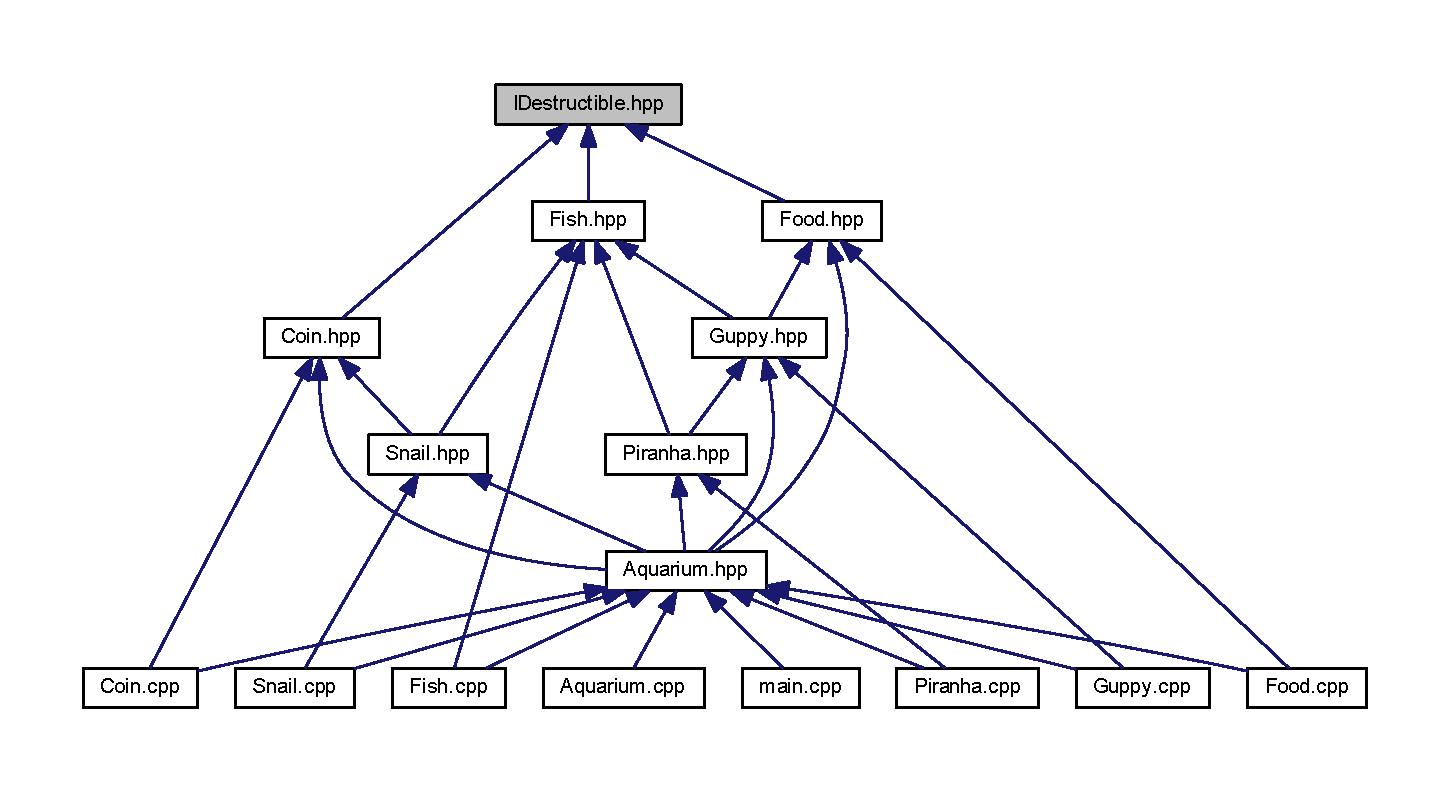
\includegraphics[width=350pt]{_i_destructible_8hpp__dep__incl}
\end{center}
\end{figure}
\subsection*{Classes}
\begin{DoxyCompactItemize}
\item 
class \mbox{\hyperlink{class_i_destructible}{I\+Destructible}}
\end{DoxyCompactItemize}

\hypertarget{_linked_list_8hpp}{}\section{Linked\+List.\+hpp File Reference}
\label{_linked_list_8hpp}\index{Linked\+List.\+hpp@{Linked\+List.\+hpp}}
This graph shows which files directly or indirectly include this file\+:
\nopagebreak
\begin{figure}[H]
\begin{center}
\leavevmode
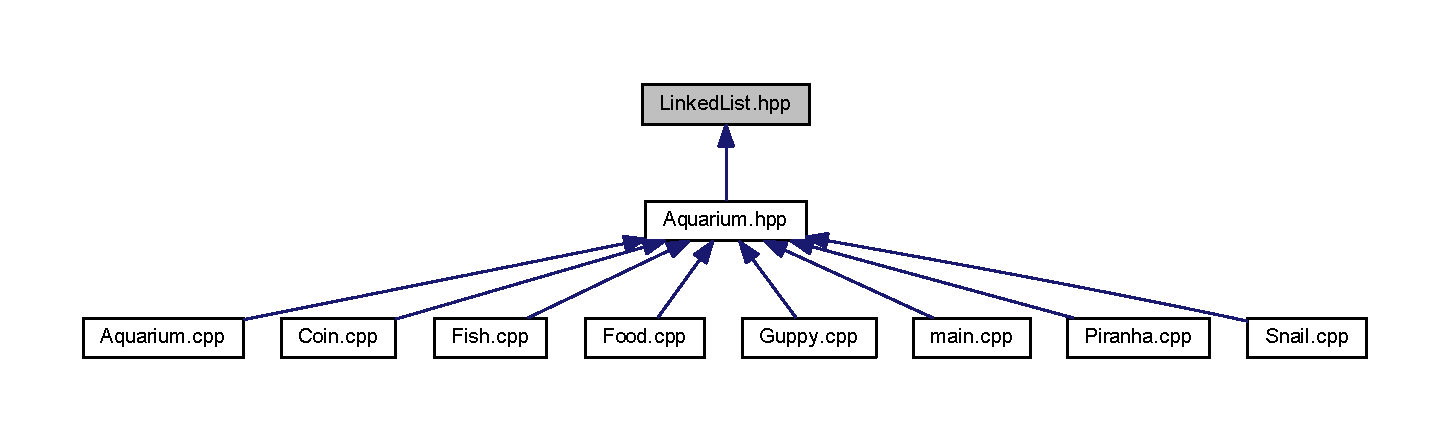
\includegraphics[width=350pt]{_linked_list_8hpp__dep__incl}
\end{center}
\end{figure}
\subsection*{Classes}
\begin{DoxyCompactItemize}
\item 
struct \mbox{\hyperlink{struct_element_list}{Element\+List$<$ T $>$}}
\item 
class \mbox{\hyperlink{class_linked_list}{Linked\+List$<$ T $>$}}
\end{DoxyCompactItemize}

\hypertarget{main_8cpp}{}\section{main.\+cpp File Reference}
\label{main_8cpp}\index{main.\+cpp@{main.\+cpp}}
{\ttfamily \#include \char`\"{}oop.\+hpp\char`\"{}}\newline
{\ttfamily \#include $<$iostream$>$}\newline
{\ttfamily \#include $<$math.\+h$>$}\newline
{\ttfamily \#include $<$sstream$>$}\newline
{\ttfamily \#include \char`\"{}Aquarium.\+hpp\char`\"{}}\newline
Include dependency graph for main.\+cpp\+:
\nopagebreak
\begin{figure}[H]
\begin{center}
\leavevmode
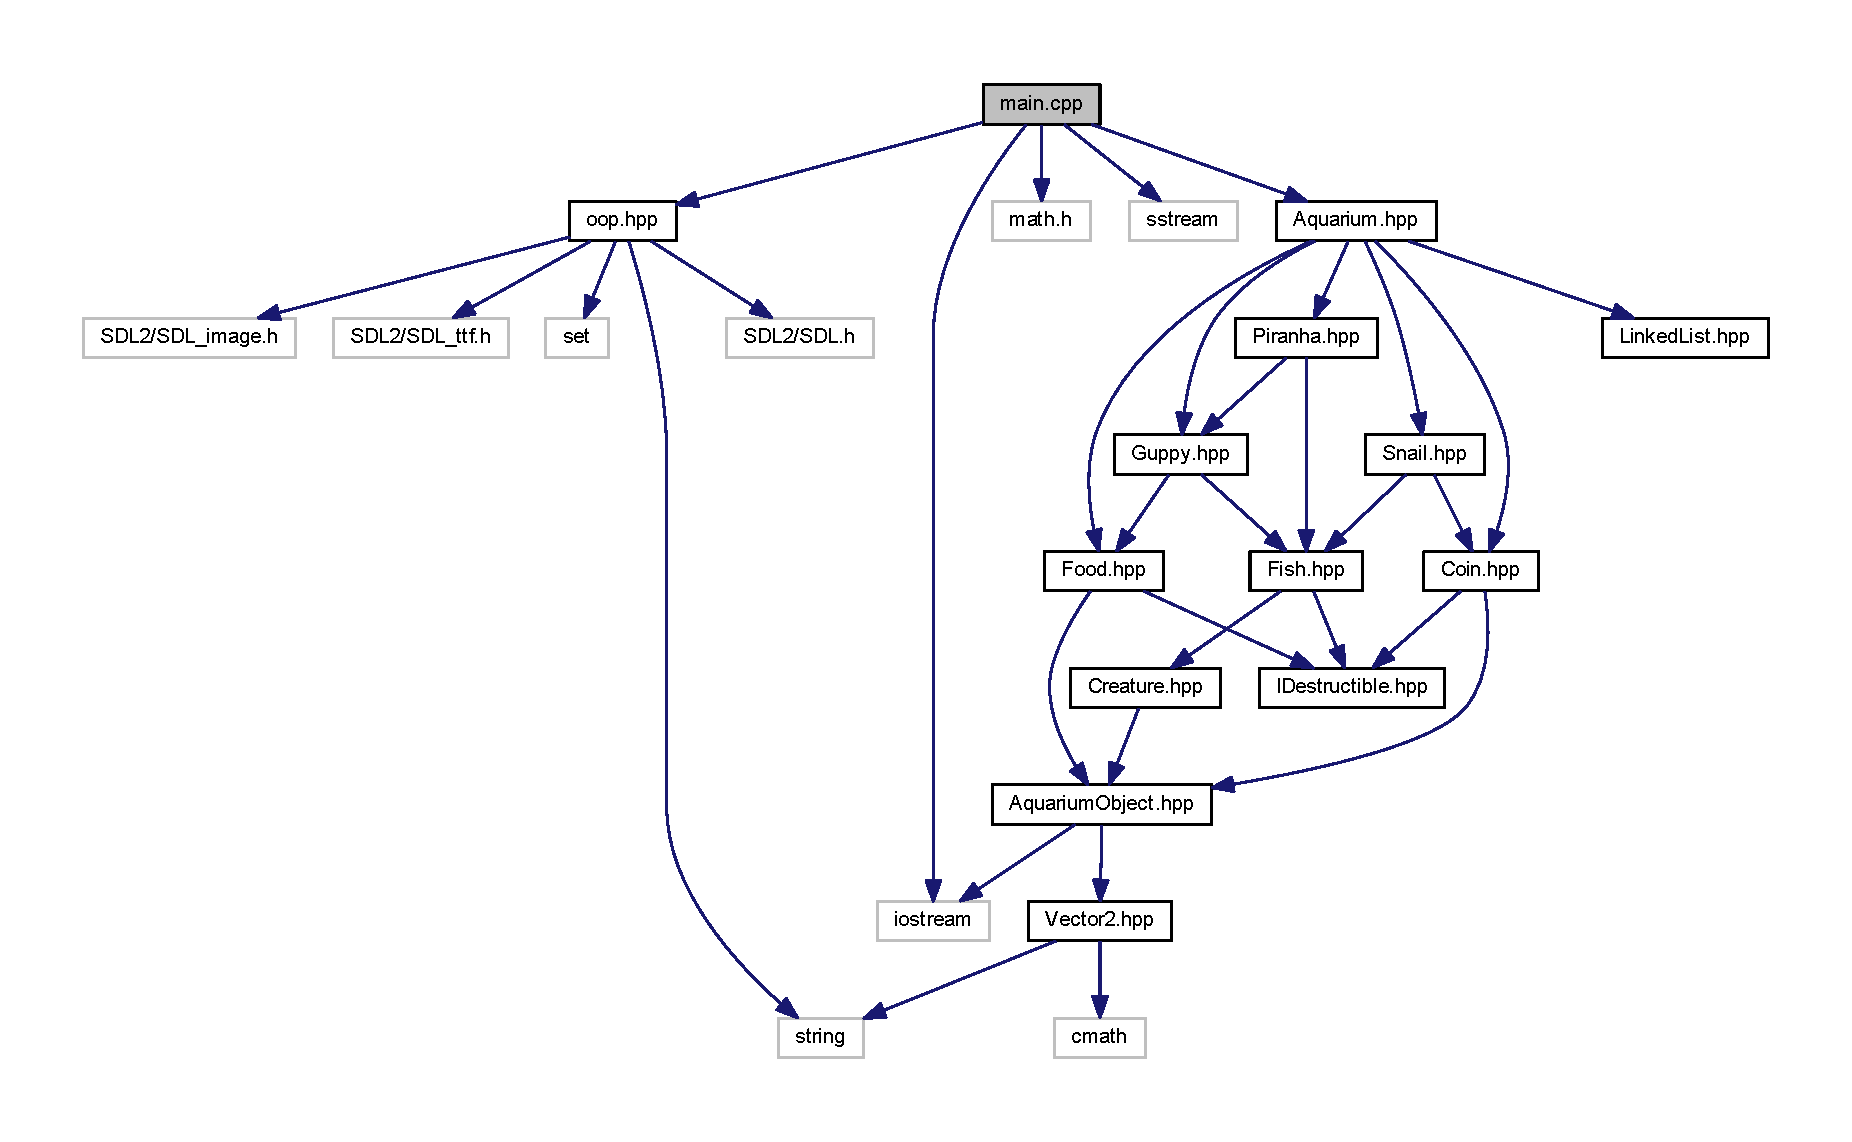
\includegraphics[width=350pt]{main_8cpp__incl}
\end{center}
\end{figure}
\subsection*{Functions}
\begin{DoxyCompactItemize}
\item 
int \mbox{\hyperlink{main_8cpp_a700a0caa5b70a06d1064e576f9f3cf65}{main}} (int argc, char $\ast$args\mbox{[}$\,$\mbox{]})
\end{DoxyCompactItemize}
\subsection*{Variables}
\begin{DoxyCompactItemize}
\item 
const double \mbox{\hyperlink{main_8cpp_a71fd37308050cd439537c5c6c2cb4614}{speed}} = 1
\item 
const double \mbox{\hyperlink{main_8cpp_a2b77d126b042f6bf66a44ce7ab5262e8}{tps}} = 20
\end{DoxyCompactItemize}


\subsection{Function Documentation}
\mbox{\Hypertarget{main_8cpp_a700a0caa5b70a06d1064e576f9f3cf65}\label{main_8cpp_a700a0caa5b70a06d1064e576f9f3cf65}} 
\index{main.\+cpp@{main.\+cpp}!main@{main}}
\index{main@{main}!main.\+cpp@{main.\+cpp}}
\subsubsection{\texorpdfstring{main()}{main()}}
{\footnotesize\ttfamily int main (\begin{DoxyParamCaption}\item[{int}]{argc,  }\item[{char $\ast$}]{args\mbox{[}$\,$\mbox{]} }\end{DoxyParamCaption})}

Main Menu

Input Handler

F\+PS Counter

Text String

Initialize Game

Game Tick

Input Handler

Update F\+PS every second

Draw

End Game

Input Handler 

\subsection{Variable Documentation}
\mbox{\Hypertarget{main_8cpp_a71fd37308050cd439537c5c6c2cb4614}\label{main_8cpp_a71fd37308050cd439537c5c6c2cb4614}} 
\index{main.\+cpp@{main.\+cpp}!speed@{speed}}
\index{speed@{speed}!main.\+cpp@{main.\+cpp}}
\subsubsection{\texorpdfstring{speed}{speed}}
{\footnotesize\ttfamily const double speed = 1}

\mbox{\Hypertarget{main_8cpp_a2b77d126b042f6bf66a44ce7ab5262e8}\label{main_8cpp_a2b77d126b042f6bf66a44ce7ab5262e8}} 
\index{main.\+cpp@{main.\+cpp}!tps@{tps}}
\index{tps@{tps}!main.\+cpp@{main.\+cpp}}
\subsubsection{\texorpdfstring{tps}{tps}}
{\footnotesize\ttfamily const double tps = 20}


\hypertarget{oop_8cpp}{}\section{oop.\+cpp File Reference}
\label{oop_8cpp}\index{oop.\+cpp@{oop.\+cpp}}
{\ttfamily \#include \char`\"{}oop.\+hpp\char`\"{}}\newline
{\ttfamily \#include $<$map$>$}\newline
{\ttfamily \#include $<$iostream$>$}\newline
{\ttfamily \#include $<$chrono$>$}\newline
Include dependency graph for oop.\+cpp\+:\nopagebreak
\begin{figure}[H]
\begin{center}
\leavevmode
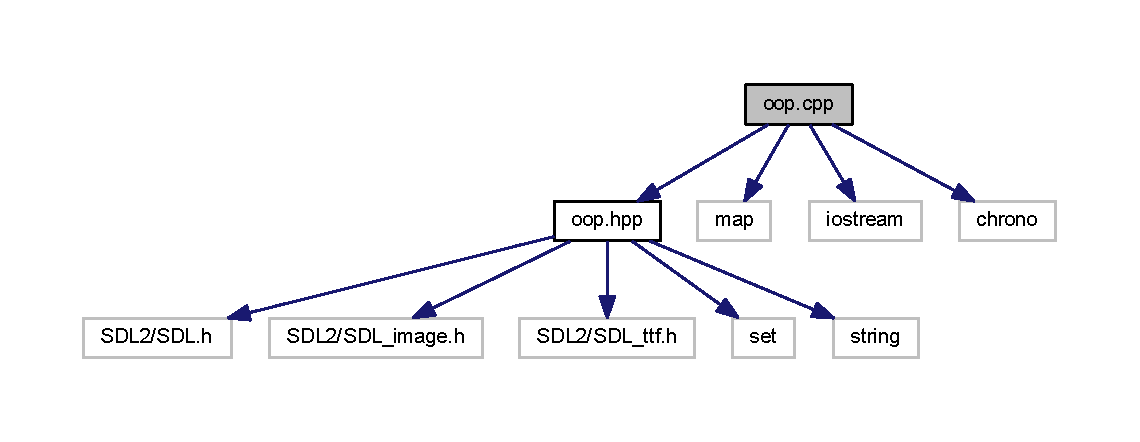
\includegraphics[width=350pt]{oop_8cpp__incl}
\end{center}
\end{figure}
\subsection*{Functions}
\begin{DoxyCompactItemize}
\item 
double \mbox{\hyperlink{oop_8cpp_a1ba1773fee3381786a816dc207a1f8d5}{time\+\_\+since\+\_\+start}} ()
\begin{DoxyCompactList}\small\item\em -\/-\/-\/-\/-\/-\/-\/-\/-\/-\/-\/-\/-\/-\/-\/-\/-\/-\/-\/-\/-\/-\/-\/-\/-\/-\/-\/-\/------ W\+A\+K\+TU -\/-\/-\/-\/-\/-\/-\/-\/-\/-\/-\/-\/-\/-\/-\/-\/-\/-\/-\/-\/-\/-\/-\/-\/-\/-\/-\/-\/------ \end{DoxyCompactList}\item 
bool \mbox{\hyperlink{oop_8cpp_aee8048628ff2b5c026c9e15acdcaacb8}{init}} ()
\begin{DoxyCompactList}\small\item\em -\/-\/-\/-\/-\/-\/-\/-\/-\/-\/-\/-\/-\/-\/-\/-\/-\/-\/-\/-\/-\/-\/-\/-\/-\/-\/-\/-\/------ S\+E\+T\+UP -\/-\/-\/-\/-\/-\/-\/-\/-\/-\/-\/-\/-\/-\/-\/-\/-\/-\/-\/-\/-\/-\/-\/-\/-\/-\/-\/-\/------ \end{DoxyCompactList}\item 
void \mbox{\hyperlink{oop_8cpp_a5ae591df94fc66ccb85cbb6565368bca}{close}} ()
\begin{DoxyCompactList}\small\item\em Menghentikan program. \end{DoxyCompactList}\item 
S\+D\+L\+\_\+\+Surface $\ast$ \mbox{\hyperlink{oop_8cpp_a0e7ac416d5997995bce4c268daa46686}{load\+Surface}} (std\+::string path)
\item 
void \mbox{\hyperlink{oop_8cpp_ab131dd50a24fc4f73642a6dbf929fea0}{draw\+\_\+background}} (std\+::string filename)
\begin{DoxyCompactList}\small\item\em -\/-\/-\/-\/-\/-\/-\/-\/-\/-\/-\/-\/-\/-\/-\/-\/-\/-\/-\/-\/-\/-\/-\/-\/------ P\+E\+N\+G\+G\+A\+M\+B\+A\+R\+AN -\/-\/-\/-\/-\/-\/-\/-\/-\/-\/-\/-\/-\/-\/-\/-\/-\/-\/-\/-\/-\/-\/-\/-\/-\/------ \end{DoxyCompactList}\item 
void \mbox{\hyperlink{oop_8cpp_a0f01596e4fd0a81c514c706c4936ee8d}{draw\+\_\+image}} (std\+::string filename, int x, int y)
\item 
void \mbox{\hyperlink{oop_8cpp_a2b13ce610f0fb0df7a95eb2307e319d2}{draw\+\_\+text}} (std\+::string text, int font\+\_\+size, int x, int y, unsigned char r, unsigned char g, unsigned char b)
\item 
void \mbox{\hyperlink{oop_8cpp_a4953d1edcbbfc7e420c423ded1d5621a}{clear\+\_\+screen}} ()
\item 
void \mbox{\hyperlink{oop_8cpp_a10da25e92e69613be93d099bb029feb2}{update\+\_\+screen}} ()
\begin{DoxyCompactList}\small\item\em Melakukan proses update terhadap layar. \end{DoxyCompactList}\item 
void \mbox{\hyperlink{oop_8cpp_ab19fbad269feb4f8cf725031233ba56e}{handle\+\_\+input}} ()
\begin{DoxyCompactList}\small\item\em -\/-\/-\/-\/-\/-\/-\/-\/-\/-\/-\/-\/-\/-\/-\/-\/-\/-\/-\/-\/-\/-\/-\/-\/-\/-\/-\/------ M\+A\+S\+U\+K\+AN -\/-\/-\/-\/-\/-\/-\/-\/-\/-\/-\/-\/-\/-\/-\/-\/-\/-\/-\/-\/-\/-\/-\/-\/-\/-\/-\/------ \end{DoxyCompactList}\item 
bool \mbox{\hyperlink{oop_8cpp_a1b14e3b0f5799f93f8dab7f5c6819298}{quit\+\_\+pressed}} ()
\item 
const std\+::set$<$ S\+D\+L\+\_\+\+Keycode $>$ \& \mbox{\hyperlink{oop_8cpp_a155dba9d2b234776d0fb743da0dcdbc2}{get\+\_\+pressed\+\_\+keys}} ()
\item 
const std\+::set$<$ S\+D\+L\+\_\+\+Keycode $>$ \& \mbox{\hyperlink{oop_8cpp_a4fdfe498ed93ea27801b69f2158e5e6a}{get\+\_\+tapped\+\_\+keys}} ()
\item 
bool \mbox{\hyperlink{oop_8cpp_a7926b3f27e93f3f8e8315a870424858e}{get\+\_\+mouse\+\_\+button\+\_\+tapped}} ()
\item 
int \mbox{\hyperlink{oop_8cpp_af7d32c587aa1e333287d138ae441c707}{get\+\_\+screen\+\_\+width}} ()
\begin{DoxyCompactList}\small\item\em Pengaturan ukuran layar yang dihasilkan. \end{DoxyCompactList}\item 
int \mbox{\hyperlink{oop_8cpp_a5eefdc1170c78252864ccef6cc723b7c}{get\+\_\+screen\+\_\+height}} ()
\end{DoxyCompactItemize}
\subsection*{Variables}
\begin{DoxyCompactItemize}
\item 
high\+\_\+resolution\+\_\+clock\+::time\+\_\+point \mbox{\hyperlink{oop_8cpp_a1735b8c468a759db2a102e031c6b1436}{start}} = high\+\_\+resolution\+\_\+clock\+::now()
\item 
S\+D\+L\+\_\+\+Window $\ast$ \mbox{\hyperlink{oop_8cpp_a7d570c1c3b1ac98019869517e6062462}{sdl\+Window}}
\item 
std\+::map$<$ std\+::string, S\+D\+L\+\_\+\+Surface $\ast$ $>$ \mbox{\hyperlink{oop_8cpp_a628cbb50ed852f954df9e6e5288b9f1c}{loaded\+Surfaces}}
\item 
std\+::map$<$ int, T\+T\+F\+\_\+\+Font $\ast$ $>$ \mbox{\hyperlink{oop_8cpp_a3dd6e6fa4b946f1a7c7325b7be30835e}{loaded\+Font\+Sizes}}
\item 
S\+D\+L\+\_\+\+Surface $\ast$ \mbox{\hyperlink{oop_8cpp_aa93b1188c9e7061fda6ed6d81cd1a774}{g\+Screen\+Surface}} = N\+U\+LL
\item 
S\+D\+L\+\_\+\+Display\+Mode \mbox{\hyperlink{oop_8cpp_afca5b7fc01b792c94e62c636f01b28a8}{current}}
\item 
bool \mbox{\hyperlink{oop_8cpp_ac746fa6ad48d19984a159f14bec028a3}{quit}} = false
\item 
std\+::set$<$ S\+D\+L\+\_\+\+Keycode $>$ \mbox{\hyperlink{oop_8cpp_a82122c0a11768870334b09ab6483f96c}{pressed\+Keys}}
\item 
std\+::set$<$ S\+D\+L\+\_\+\+Keycode $>$ \mbox{\hyperlink{oop_8cpp_afee38be0153d2eb7d46f4f1fd9d3dc8b}{tapped\+Keys}}
\item 
bool \mbox{\hyperlink{oop_8cpp_ad524f283eebfb29ba63695313a8b3da8}{mouse\+Button\+Tapped}}
\end{DoxyCompactItemize}


\subsection{Function Documentation}
\mbox{\Hypertarget{oop_8cpp_a4953d1edcbbfc7e420c423ded1d5621a}\label{oop_8cpp_a4953d1edcbbfc7e420c423ded1d5621a}} 
\index{oop.\+cpp@{oop.\+cpp}!clear\+\_\+screen@{clear\+\_\+screen}}
\index{clear\+\_\+screen@{clear\+\_\+screen}!oop.\+cpp@{oop.\+cpp}}
\subsubsection{\texorpdfstring{clear\+\_\+screen()}{clear\_screen()}}
{\footnotesize\ttfamily void clear\+\_\+screen (\begin{DoxyParamCaption}{ }\end{DoxyParamCaption})}

Mengisi layar dengan warna putih. Perubahan di layar baru muncul ketika \mbox{\hyperlink{oop_8hpp_a10da25e92e69613be93d099bb029feb2}{update\+\_\+screen()}} dipanggil. \mbox{\Hypertarget{oop_8cpp_a5ae591df94fc66ccb85cbb6565368bca}\label{oop_8cpp_a5ae591df94fc66ccb85cbb6565368bca}} 
\index{oop.\+cpp@{oop.\+cpp}!close@{close}}
\index{close@{close}!oop.\+cpp@{oop.\+cpp}}
\subsubsection{\texorpdfstring{close()}{close()}}
{\footnotesize\ttfamily void close (\begin{DoxyParamCaption}{ }\end{DoxyParamCaption})}



Menghentikan program. 

\mbox{\Hypertarget{oop_8cpp_ab131dd50a24fc4f73642a6dbf929fea0}\label{oop_8cpp_ab131dd50a24fc4f73642a6dbf929fea0}} 
\index{oop.\+cpp@{oop.\+cpp}!draw\+\_\+background@{draw\+\_\+background}}
\index{draw\+\_\+background@{draw\+\_\+background}!oop.\+cpp@{oop.\+cpp}}
\subsubsection{\texorpdfstring{draw\+\_\+background()}{draw\_background()}}
{\footnotesize\ttfamily void draw\+\_\+background (\begin{DoxyParamCaption}\item[{std\+::string}]{filename }\end{DoxyParamCaption})}



-\/-\/-\/-\/-\/-\/-\/-\/-\/-\/-\/-\/-\/-\/-\/-\/-\/-\/-\/-\/-\/-\/-\/-\/------ P\+E\+N\+G\+G\+A\+M\+B\+A\+R\+AN -\/-\/-\/-\/-\/-\/-\/-\/-\/-\/-\/-\/-\/-\/-\/-\/-\/-\/-\/-\/-\/-\/-\/-\/-\/------ 

Menggambar suatu gambar png, jpg, bmp sehingga gambar mengisi layar Perubahan di layar baru muncul ketika \mbox{\hyperlink{oop_8hpp_a10da25e92e69613be93d099bb029feb2}{update\+\_\+screen()}} dipanggil. \mbox{\Hypertarget{oop_8cpp_a0f01596e4fd0a81c514c706c4936ee8d}\label{oop_8cpp_a0f01596e4fd0a81c514c706c4936ee8d}} 
\index{oop.\+cpp@{oop.\+cpp}!draw\+\_\+image@{draw\+\_\+image}}
\index{draw\+\_\+image@{draw\+\_\+image}!oop.\+cpp@{oop.\+cpp}}
\subsubsection{\texorpdfstring{draw\+\_\+image()}{draw\_image()}}
{\footnotesize\ttfamily void draw\+\_\+image (\begin{DoxyParamCaption}\item[{std\+::string}]{filename,  }\item[{int}]{x,  }\item[{int}]{y }\end{DoxyParamCaption})}

Menggambar suatu gambar png, jpg, bmp sehingga tengah gambar berada di titik (x, y). Perubahan di layar baru muncul ketika \mbox{\hyperlink{oop_8hpp_a10da25e92e69613be93d099bb029feb2}{update\+\_\+screen()}} dipanggil. \mbox{\Hypertarget{oop_8cpp_a2b13ce610f0fb0df7a95eb2307e319d2}\label{oop_8cpp_a2b13ce610f0fb0df7a95eb2307e319d2}} 
\index{oop.\+cpp@{oop.\+cpp}!draw\+\_\+text@{draw\+\_\+text}}
\index{draw\+\_\+text@{draw\+\_\+text}!oop.\+cpp@{oop.\+cpp}}
\subsubsection{\texorpdfstring{draw\+\_\+text()}{draw\_text()}}
{\footnotesize\ttfamily void draw\+\_\+text (\begin{DoxyParamCaption}\item[{std\+::string}]{text,  }\item[{int}]{font\+\_\+size,  }\item[{int}]{x,  }\item[{int}]{y,  }\item[{unsigned char}]{r,  }\item[{unsigned char}]{g,  }\item[{unsigned char}]{b }\end{DoxyParamCaption})}

Menuliskan teks berukuran font\+\_\+size berwarna (r, g, b) ke layar sehingga kiri atas teks berada di titik (x, y). Perubahan di layar baru muncul ketika \mbox{\hyperlink{oop_8hpp_a10da25e92e69613be93d099bb029feb2}{update\+\_\+screen()}} dipanggil. \mbox{\Hypertarget{oop_8cpp_a7926b3f27e93f3f8e8315a870424858e}\label{oop_8cpp_a7926b3f27e93f3f8e8315a870424858e}} 
\index{oop.\+cpp@{oop.\+cpp}!get\+\_\+mouse\+\_\+button\+\_\+tapped@{get\+\_\+mouse\+\_\+button\+\_\+tapped}}
\index{get\+\_\+mouse\+\_\+button\+\_\+tapped@{get\+\_\+mouse\+\_\+button\+\_\+tapped}!oop.\+cpp@{oop.\+cpp}}
\subsubsection{\texorpdfstring{get\+\_\+mouse\+\_\+button\+\_\+tapped()}{get\_mouse\_button\_tapped()}}
{\footnotesize\ttfamily bool get\+\_\+mouse\+\_\+button\+\_\+tapped (\begin{DoxyParamCaption}{ }\end{DoxyParamCaption})}

\mbox{\Hypertarget{oop_8cpp_a155dba9d2b234776d0fb743da0dcdbc2}\label{oop_8cpp_a155dba9d2b234776d0fb743da0dcdbc2}} 
\index{oop.\+cpp@{oop.\+cpp}!get\+\_\+pressed\+\_\+keys@{get\+\_\+pressed\+\_\+keys}}
\index{get\+\_\+pressed\+\_\+keys@{get\+\_\+pressed\+\_\+keys}!oop.\+cpp@{oop.\+cpp}}
\subsubsection{\texorpdfstring{get\+\_\+pressed\+\_\+keys()}{get\_pressed\_keys()}}
{\footnotesize\ttfamily const std\+::set$<$S\+D\+L\+\_\+\+Keycode$>$\& get\+\_\+pressed\+\_\+keys (\begin{DoxyParamCaption}{ }\end{DoxyParamCaption})}

Untuk dua fungsi berikut, nama konstan kode yang tepat dapat dilihat di \href{https://wiki.libsdl.org/SDL_Keycode}{\tt https\+://wiki.\+libsdl.\+org/\+S\+D\+L\+\_\+\+Keycode} pada kolom \char`\"{}\+S\+D\+L\+\_\+\+Keycode Value\char`\"{}. Mengembalikan himpunan kode tombol yang sedang ditekan pada saat \mbox{\hyperlink{oop_8hpp_ab19fbad269feb4f8cf725031233ba56e}{handle\+\_\+input()}} terakhir dipanggil. \mbox{\Hypertarget{oop_8cpp_a5eefdc1170c78252864ccef6cc723b7c}\label{oop_8cpp_a5eefdc1170c78252864ccef6cc723b7c}} 
\index{oop.\+cpp@{oop.\+cpp}!get\+\_\+screen\+\_\+height@{get\+\_\+screen\+\_\+height}}
\index{get\+\_\+screen\+\_\+height@{get\+\_\+screen\+\_\+height}!oop.\+cpp@{oop.\+cpp}}
\subsubsection{\texorpdfstring{get\+\_\+screen\+\_\+height()}{get\_screen\_height()}}
{\footnotesize\ttfamily int get\+\_\+screen\+\_\+height (\begin{DoxyParamCaption}{ }\end{DoxyParamCaption})}

\mbox{\Hypertarget{oop_8cpp_af7d32c587aa1e333287d138ae441c707}\label{oop_8cpp_af7d32c587aa1e333287d138ae441c707}} 
\index{oop.\+cpp@{oop.\+cpp}!get\+\_\+screen\+\_\+width@{get\+\_\+screen\+\_\+width}}
\index{get\+\_\+screen\+\_\+width@{get\+\_\+screen\+\_\+width}!oop.\+cpp@{oop.\+cpp}}
\subsubsection{\texorpdfstring{get\+\_\+screen\+\_\+width()}{get\_screen\_width()}}
{\footnotesize\ttfamily int get\+\_\+screen\+\_\+width (\begin{DoxyParamCaption}{ }\end{DoxyParamCaption})}



Pengaturan ukuran layar yang dihasilkan. 

\mbox{\Hypertarget{oop_8cpp_a4fdfe498ed93ea27801b69f2158e5e6a}\label{oop_8cpp_a4fdfe498ed93ea27801b69f2158e5e6a}} 
\index{oop.\+cpp@{oop.\+cpp}!get\+\_\+tapped\+\_\+keys@{get\+\_\+tapped\+\_\+keys}}
\index{get\+\_\+tapped\+\_\+keys@{get\+\_\+tapped\+\_\+keys}!oop.\+cpp@{oop.\+cpp}}
\subsubsection{\texorpdfstring{get\+\_\+tapped\+\_\+keys()}{get\_tapped\_keys()}}
{\footnotesize\ttfamily const std\+::set$<$S\+D\+L\+\_\+\+Keycode$>$\& get\+\_\+tapped\+\_\+keys (\begin{DoxyParamCaption}{ }\end{DoxyParamCaption})}

Mengembalikan himpunan kode tombol yang baru mulai ditekan pada saat \mbox{\hyperlink{oop_8hpp_ab19fbad269feb4f8cf725031233ba56e}{handle\+\_\+input()}} terakhir dipanggil. \mbox{\Hypertarget{oop_8cpp_ab19fbad269feb4f8cf725031233ba56e}\label{oop_8cpp_ab19fbad269feb4f8cf725031233ba56e}} 
\index{oop.\+cpp@{oop.\+cpp}!handle\+\_\+input@{handle\+\_\+input}}
\index{handle\+\_\+input@{handle\+\_\+input}!oop.\+cpp@{oop.\+cpp}}
\subsubsection{\texorpdfstring{handle\+\_\+input()}{handle\_input()}}
{\footnotesize\ttfamily void handle\+\_\+input (\begin{DoxyParamCaption}{ }\end{DoxyParamCaption})}



-\/-\/-\/-\/-\/-\/-\/-\/-\/-\/-\/-\/-\/-\/-\/-\/-\/-\/-\/-\/-\/-\/-\/-\/-\/-\/-\/------ M\+A\+S\+U\+K\+AN -\/-\/-\/-\/-\/-\/-\/-\/-\/-\/-\/-\/-\/-\/-\/-\/-\/-\/-\/-\/-\/-\/-\/-\/-\/-\/-\/------ 

Memproses masukan dari sistem operasi. \mbox{\Hypertarget{oop_8cpp_aee8048628ff2b5c026c9e15acdcaacb8}\label{oop_8cpp_aee8048628ff2b5c026c9e15acdcaacb8}} 
\index{oop.\+cpp@{oop.\+cpp}!init@{init}}
\index{init@{init}!oop.\+cpp@{oop.\+cpp}}
\subsubsection{\texorpdfstring{init()}{init()}}
{\footnotesize\ttfamily bool init (\begin{DoxyParamCaption}{ }\end{DoxyParamCaption})}



-\/-\/-\/-\/-\/-\/-\/-\/-\/-\/-\/-\/-\/-\/-\/-\/-\/-\/-\/-\/-\/-\/-\/-\/-\/-\/-\/-\/------ S\+E\+T\+UP -\/-\/-\/-\/-\/-\/-\/-\/-\/-\/-\/-\/-\/-\/-\/-\/-\/-\/-\/-\/-\/-\/-\/-\/-\/-\/-\/-\/------ 

Melakukan inisialisasi terhadap program. \mbox{\Hypertarget{oop_8cpp_a0e7ac416d5997995bce4c268daa46686}\label{oop_8cpp_a0e7ac416d5997995bce4c268daa46686}} 
\index{oop.\+cpp@{oop.\+cpp}!load\+Surface@{load\+Surface}}
\index{load\+Surface@{load\+Surface}!oop.\+cpp@{oop.\+cpp}}
\subsubsection{\texorpdfstring{load\+Surface()}{loadSurface()}}
{\footnotesize\ttfamily S\+D\+L\+\_\+\+Surface$\ast$ load\+Surface (\begin{DoxyParamCaption}\item[{std\+::string}]{path }\end{DoxyParamCaption})}

\mbox{\Hypertarget{oop_8cpp_a1b14e3b0f5799f93f8dab7f5c6819298}\label{oop_8cpp_a1b14e3b0f5799f93f8dab7f5c6819298}} 
\index{oop.\+cpp@{oop.\+cpp}!quit\+\_\+pressed@{quit\+\_\+pressed}}
\index{quit\+\_\+pressed@{quit\+\_\+pressed}!oop.\+cpp@{oop.\+cpp}}
\subsubsection{\texorpdfstring{quit\+\_\+pressed()}{quit\_pressed()}}
{\footnotesize\ttfamily bool quit\+\_\+pressed (\begin{DoxyParamCaption}{ }\end{DoxyParamCaption})}

Mengembalikan apakah pengguna telah meminta keluar dengan menekan tombol keluar di jendela program ketika \mbox{\hyperlink{oop_8hpp_ab19fbad269feb4f8cf725031233ba56e}{handle\+\_\+input()}} terakhir dipanggil. \mbox{\Hypertarget{oop_8cpp_a1ba1773fee3381786a816dc207a1f8d5}\label{oop_8cpp_a1ba1773fee3381786a816dc207a1f8d5}} 
\index{oop.\+cpp@{oop.\+cpp}!time\+\_\+since\+\_\+start@{time\+\_\+since\+\_\+start}}
\index{time\+\_\+since\+\_\+start@{time\+\_\+since\+\_\+start}!oop.\+cpp@{oop.\+cpp}}
\subsubsection{\texorpdfstring{time\+\_\+since\+\_\+start()}{time\_since\_start()}}
{\footnotesize\ttfamily double time\+\_\+since\+\_\+start (\begin{DoxyParamCaption}{ }\end{DoxyParamCaption})}



-\/-\/-\/-\/-\/-\/-\/-\/-\/-\/-\/-\/-\/-\/-\/-\/-\/-\/-\/-\/-\/-\/-\/-\/-\/-\/-\/-\/------ W\+A\+K\+TU -\/-\/-\/-\/-\/-\/-\/-\/-\/-\/-\/-\/-\/-\/-\/-\/-\/-\/-\/-\/-\/-\/-\/-\/-\/-\/-\/-\/------ 

Mengembalikan waktu dari permulaan program dalam nilai detik (bisa pecahan). \mbox{\Hypertarget{oop_8cpp_a10da25e92e69613be93d099bb029feb2}\label{oop_8cpp_a10da25e92e69613be93d099bb029feb2}} 
\index{oop.\+cpp@{oop.\+cpp}!update\+\_\+screen@{update\+\_\+screen}}
\index{update\+\_\+screen@{update\+\_\+screen}!oop.\+cpp@{oop.\+cpp}}
\subsubsection{\texorpdfstring{update\+\_\+screen()}{update\_screen()}}
{\footnotesize\ttfamily void update\+\_\+screen (\begin{DoxyParamCaption}{ }\end{DoxyParamCaption})}



Melakukan proses update terhadap layar. 



\subsection{Variable Documentation}
\mbox{\Hypertarget{oop_8cpp_afca5b7fc01b792c94e62c636f01b28a8}\label{oop_8cpp_afca5b7fc01b792c94e62c636f01b28a8}} 
\index{oop.\+cpp@{oop.\+cpp}!current@{current}}
\index{current@{current}!oop.\+cpp@{oop.\+cpp}}
\subsubsection{\texorpdfstring{current}{current}}
{\footnotesize\ttfamily S\+D\+L\+\_\+\+Display\+Mode current}

\mbox{\Hypertarget{oop_8cpp_aa93b1188c9e7061fda6ed6d81cd1a774}\label{oop_8cpp_aa93b1188c9e7061fda6ed6d81cd1a774}} 
\index{oop.\+cpp@{oop.\+cpp}!g\+Screen\+Surface@{g\+Screen\+Surface}}
\index{g\+Screen\+Surface@{g\+Screen\+Surface}!oop.\+cpp@{oop.\+cpp}}
\subsubsection{\texorpdfstring{g\+Screen\+Surface}{gScreenSurface}}
{\footnotesize\ttfamily S\+D\+L\+\_\+\+Surface$\ast$ g\+Screen\+Surface = N\+U\+LL}

\mbox{\Hypertarget{oop_8cpp_a3dd6e6fa4b946f1a7c7325b7be30835e}\label{oop_8cpp_a3dd6e6fa4b946f1a7c7325b7be30835e}} 
\index{oop.\+cpp@{oop.\+cpp}!loaded\+Font\+Sizes@{loaded\+Font\+Sizes}}
\index{loaded\+Font\+Sizes@{loaded\+Font\+Sizes}!oop.\+cpp@{oop.\+cpp}}
\subsubsection{\texorpdfstring{loaded\+Font\+Sizes}{loadedFontSizes}}
{\footnotesize\ttfamily std\+::map$<$int, T\+T\+F\+\_\+\+Font$\ast$$>$ loaded\+Font\+Sizes}

\mbox{\Hypertarget{oop_8cpp_a628cbb50ed852f954df9e6e5288b9f1c}\label{oop_8cpp_a628cbb50ed852f954df9e6e5288b9f1c}} 
\index{oop.\+cpp@{oop.\+cpp}!loaded\+Surfaces@{loaded\+Surfaces}}
\index{loaded\+Surfaces@{loaded\+Surfaces}!oop.\+cpp@{oop.\+cpp}}
\subsubsection{\texorpdfstring{loaded\+Surfaces}{loadedSurfaces}}
{\footnotesize\ttfamily std\+::map$<$std\+::string, S\+D\+L\+\_\+\+Surface$\ast$$>$ loaded\+Surfaces}

\mbox{\Hypertarget{oop_8cpp_ad524f283eebfb29ba63695313a8b3da8}\label{oop_8cpp_ad524f283eebfb29ba63695313a8b3da8}} 
\index{oop.\+cpp@{oop.\+cpp}!mouse\+Button\+Tapped@{mouse\+Button\+Tapped}}
\index{mouse\+Button\+Tapped@{mouse\+Button\+Tapped}!oop.\+cpp@{oop.\+cpp}}
\subsubsection{\texorpdfstring{mouse\+Button\+Tapped}{mouseButtonTapped}}
{\footnotesize\ttfamily bool mouse\+Button\+Tapped}

\mbox{\Hypertarget{oop_8cpp_a82122c0a11768870334b09ab6483f96c}\label{oop_8cpp_a82122c0a11768870334b09ab6483f96c}} 
\index{oop.\+cpp@{oop.\+cpp}!pressed\+Keys@{pressed\+Keys}}
\index{pressed\+Keys@{pressed\+Keys}!oop.\+cpp@{oop.\+cpp}}
\subsubsection{\texorpdfstring{pressed\+Keys}{pressedKeys}}
{\footnotesize\ttfamily std\+::set$<$S\+D\+L\+\_\+\+Keycode$>$ pressed\+Keys}

\mbox{\Hypertarget{oop_8cpp_ac746fa6ad48d19984a159f14bec028a3}\label{oop_8cpp_ac746fa6ad48d19984a159f14bec028a3}} 
\index{oop.\+cpp@{oop.\+cpp}!quit@{quit}}
\index{quit@{quit}!oop.\+cpp@{oop.\+cpp}}
\subsubsection{\texorpdfstring{quit}{quit}}
{\footnotesize\ttfamily bool quit = false}

\mbox{\Hypertarget{oop_8cpp_a7d570c1c3b1ac98019869517e6062462}\label{oop_8cpp_a7d570c1c3b1ac98019869517e6062462}} 
\index{oop.\+cpp@{oop.\+cpp}!sdl\+Window@{sdl\+Window}}
\index{sdl\+Window@{sdl\+Window}!oop.\+cpp@{oop.\+cpp}}
\subsubsection{\texorpdfstring{sdl\+Window}{sdlWindow}}
{\footnotesize\ttfamily S\+D\+L\+\_\+\+Window$\ast$ sdl\+Window}

\mbox{\Hypertarget{oop_8cpp_a1735b8c468a759db2a102e031c6b1436}\label{oop_8cpp_a1735b8c468a759db2a102e031c6b1436}} 
\index{oop.\+cpp@{oop.\+cpp}!start@{start}}
\index{start@{start}!oop.\+cpp@{oop.\+cpp}}
\subsubsection{\texorpdfstring{start}{start}}
{\footnotesize\ttfamily high\+\_\+resolution\+\_\+clock\+::time\+\_\+point start = high\+\_\+resolution\+\_\+clock\+::now()}

\mbox{\Hypertarget{oop_8cpp_afee38be0153d2eb7d46f4f1fd9d3dc8b}\label{oop_8cpp_afee38be0153d2eb7d46f4f1fd9d3dc8b}} 
\index{oop.\+cpp@{oop.\+cpp}!tapped\+Keys@{tapped\+Keys}}
\index{tapped\+Keys@{tapped\+Keys}!oop.\+cpp@{oop.\+cpp}}
\subsubsection{\texorpdfstring{tapped\+Keys}{tappedKeys}}
{\footnotesize\ttfamily std\+::set$<$S\+D\+L\+\_\+\+Keycode$>$ tapped\+Keys}


\hypertarget{oop_8hpp}{}\section{oop.\+hpp File Reference}
\label{oop_8hpp}\index{oop.\+hpp@{oop.\+hpp}}
{\ttfamily \#include $<$S\+D\+L2/\+S\+D\+L.\+h$>$}\newline
{\ttfamily \#include $<$S\+D\+L2/\+S\+D\+L\+\_\+image.\+h$>$}\newline
{\ttfamily \#include $<$S\+D\+L2/\+S\+D\+L\+\_\+ttf.\+h$>$}\newline
{\ttfamily \#include $<$set$>$}\newline
{\ttfamily \#include $<$string$>$}\newline
Include dependency graph for oop.\+hpp\+:
\nopagebreak
\begin{figure}[H]
\begin{center}
\leavevmode
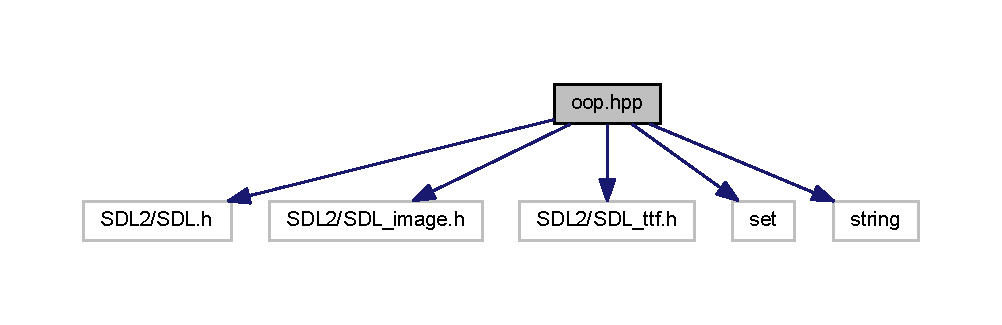
\includegraphics[width=350pt]{oop_8hpp__incl}
\end{center}
\end{figure}
This graph shows which files directly or indirectly include this file\+:
\nopagebreak
\begin{figure}[H]
\begin{center}
\leavevmode
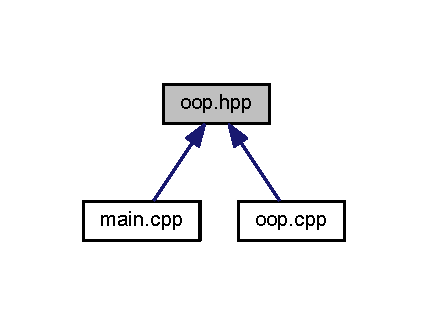
\includegraphics[width=206pt]{oop_8hpp__dep__incl}
\end{center}
\end{figure}
\subsection*{Functions}
\begin{DoxyCompactItemize}
\item 
int \mbox{\hyperlink{oop_8hpp_af7d32c587aa1e333287d138ae441c707}{get\+\_\+screen\+\_\+width}} ()
\begin{DoxyCompactList}\small\item\em Pengaturan ukuran layar yang dihasilkan. \end{DoxyCompactList}\item 
int \mbox{\hyperlink{oop_8hpp_a5eefdc1170c78252864ccef6cc723b7c}{get\+\_\+screen\+\_\+height}} ()
\item 
bool \mbox{\hyperlink{oop_8hpp_aee8048628ff2b5c026c9e15acdcaacb8}{init}} ()
\begin{DoxyCompactList}\small\item\em -\/-\/-\/-\/-\/-\/-\/-\/-\/-\/-\/-\/-\/-\/-\/-\/-\/-\/-\/-\/-\/-\/-\/-\/-\/-\/-\/-\/------ S\+E\+T\+UP -\/-\/-\/-\/-\/-\/-\/-\/-\/-\/-\/-\/-\/-\/-\/-\/-\/-\/-\/-\/-\/-\/-\/-\/-\/-\/-\/-\/------ \end{DoxyCompactList}\item 
void \mbox{\hyperlink{oop_8hpp_a5ae591df94fc66ccb85cbb6565368bca}{close}} ()
\begin{DoxyCompactList}\small\item\em Menghentikan program. \end{DoxyCompactList}\item 
void \mbox{\hyperlink{oop_8hpp_ab131dd50a24fc4f73642a6dbf929fea0}{draw\+\_\+background}} (std\+::string filename)
\begin{DoxyCompactList}\small\item\em -\/-\/-\/-\/-\/-\/-\/-\/-\/-\/-\/-\/-\/-\/-\/-\/-\/-\/-\/-\/-\/-\/-\/-\/------ P\+E\+N\+G\+G\+A\+M\+B\+A\+R\+AN -\/-\/-\/-\/-\/-\/-\/-\/-\/-\/-\/-\/-\/-\/-\/-\/-\/-\/-\/-\/-\/-\/-\/-\/-\/------ \end{DoxyCompactList}\item 
void \mbox{\hyperlink{oop_8hpp_a0f01596e4fd0a81c514c706c4936ee8d}{draw\+\_\+image}} (std\+::string filename, int x, int y)
\item 
void \mbox{\hyperlink{oop_8hpp_a2b13ce610f0fb0df7a95eb2307e319d2}{draw\+\_\+text}} (std\+::string text, int font\+\_\+size, int x, int y, unsigned char r, unsigned char g, unsigned char b)
\item 
void \mbox{\hyperlink{oop_8hpp_a4953d1edcbbfc7e420c423ded1d5621a}{clear\+\_\+screen}} ()
\item 
void \mbox{\hyperlink{oop_8hpp_a10da25e92e69613be93d099bb029feb2}{update\+\_\+screen}} ()
\begin{DoxyCompactList}\small\item\em Melakukan proses update terhadap layar. \end{DoxyCompactList}\item 
void \mbox{\hyperlink{oop_8hpp_ab19fbad269feb4f8cf725031233ba56e}{handle\+\_\+input}} ()
\begin{DoxyCompactList}\small\item\em -\/-\/-\/-\/-\/-\/-\/-\/-\/-\/-\/-\/-\/-\/-\/-\/-\/-\/-\/-\/-\/-\/-\/-\/-\/-\/-\/------ M\+A\+S\+U\+K\+AN -\/-\/-\/-\/-\/-\/-\/-\/-\/-\/-\/-\/-\/-\/-\/-\/-\/-\/-\/-\/-\/-\/-\/-\/-\/-\/-\/------ \end{DoxyCompactList}\item 
bool \mbox{\hyperlink{oop_8hpp_a1b14e3b0f5799f93f8dab7f5c6819298}{quit\+\_\+pressed}} ()
\item 
const std\+::set$<$ S\+D\+L\+\_\+\+Keycode $>$ \& \mbox{\hyperlink{oop_8hpp_a155dba9d2b234776d0fb743da0dcdbc2}{get\+\_\+pressed\+\_\+keys}} ()
\item 
const std\+::set$<$ S\+D\+L\+\_\+\+Keycode $>$ \& \mbox{\hyperlink{oop_8hpp_a4fdfe498ed93ea27801b69f2158e5e6a}{get\+\_\+tapped\+\_\+keys}} ()
\item 
bool \mbox{\hyperlink{oop_8hpp_a7926b3f27e93f3f8e8315a870424858e}{get\+\_\+mouse\+\_\+button\+\_\+tapped}} ()
\item 
double \mbox{\hyperlink{oop_8hpp_a1ba1773fee3381786a816dc207a1f8d5}{time\+\_\+since\+\_\+start}} ()
\begin{DoxyCompactList}\small\item\em -\/-\/-\/-\/-\/-\/-\/-\/-\/-\/-\/-\/-\/-\/-\/-\/-\/-\/-\/-\/-\/-\/-\/-\/-\/-\/-\/-\/------ W\+A\+K\+TU -\/-\/-\/-\/-\/-\/-\/-\/-\/-\/-\/-\/-\/-\/-\/-\/-\/-\/-\/-\/-\/-\/-\/-\/-\/-\/-\/-\/------ \end{DoxyCompactList}\end{DoxyCompactItemize}
\subsection*{Variables}
\begin{DoxyCompactItemize}
\item 
const char $\ast$const \mbox{\hyperlink{oop_8hpp_aa138e55e1cd5980069d8a26538b96fd3}{F\+O\+N\+T\+\_\+\+N\+A\+ME}} = \char`\"{}Open\+Sans-\/Regular.\+ttf\char`\"{}
\begin{DoxyCompactList}\small\item\em Nama font yang digunakan untuk menggambar tulisan. \end{DoxyCompactList}\end{DoxyCompactItemize}


\subsection{Function Documentation}
\mbox{\Hypertarget{oop_8hpp_a4953d1edcbbfc7e420c423ded1d5621a}\label{oop_8hpp_a4953d1edcbbfc7e420c423ded1d5621a}} 
\index{oop.\+hpp@{oop.\+hpp}!clear\+\_\+screen@{clear\+\_\+screen}}
\index{clear\+\_\+screen@{clear\+\_\+screen}!oop.\+hpp@{oop.\+hpp}}
\subsubsection{\texorpdfstring{clear\+\_\+screen()}{clear\_screen()}}
{\footnotesize\ttfamily void clear\+\_\+screen (\begin{DoxyParamCaption}{ }\end{DoxyParamCaption})}

Mengisi layar dengan warna putih. Perubahan di layar baru muncul ketika \mbox{\hyperlink{oop_8hpp_a10da25e92e69613be93d099bb029feb2}{update\+\_\+screen()}} dipanggil. \mbox{\Hypertarget{oop_8hpp_a5ae591df94fc66ccb85cbb6565368bca}\label{oop_8hpp_a5ae591df94fc66ccb85cbb6565368bca}} 
\index{oop.\+hpp@{oop.\+hpp}!close@{close}}
\index{close@{close}!oop.\+hpp@{oop.\+hpp}}
\subsubsection{\texorpdfstring{close()}{close()}}
{\footnotesize\ttfamily void close (\begin{DoxyParamCaption}{ }\end{DoxyParamCaption})}



Menghentikan program. 

\mbox{\Hypertarget{oop_8hpp_ab131dd50a24fc4f73642a6dbf929fea0}\label{oop_8hpp_ab131dd50a24fc4f73642a6dbf929fea0}} 
\index{oop.\+hpp@{oop.\+hpp}!draw\+\_\+background@{draw\+\_\+background}}
\index{draw\+\_\+background@{draw\+\_\+background}!oop.\+hpp@{oop.\+hpp}}
\subsubsection{\texorpdfstring{draw\+\_\+background()}{draw\_background()}}
{\footnotesize\ttfamily void draw\+\_\+background (\begin{DoxyParamCaption}\item[{std\+::string}]{filename }\end{DoxyParamCaption})}



-\/-\/-\/-\/-\/-\/-\/-\/-\/-\/-\/-\/-\/-\/-\/-\/-\/-\/-\/-\/-\/-\/-\/-\/------ P\+E\+N\+G\+G\+A\+M\+B\+A\+R\+AN -\/-\/-\/-\/-\/-\/-\/-\/-\/-\/-\/-\/-\/-\/-\/-\/-\/-\/-\/-\/-\/-\/-\/-\/-\/------ 

Menggambar suatu gambar png, jpg, bmp sehingga gambar mengisi layar Perubahan di layar baru muncul ketika \mbox{\hyperlink{oop_8hpp_a10da25e92e69613be93d099bb029feb2}{update\+\_\+screen()}} dipanggil. \mbox{\Hypertarget{oop_8hpp_a0f01596e4fd0a81c514c706c4936ee8d}\label{oop_8hpp_a0f01596e4fd0a81c514c706c4936ee8d}} 
\index{oop.\+hpp@{oop.\+hpp}!draw\+\_\+image@{draw\+\_\+image}}
\index{draw\+\_\+image@{draw\+\_\+image}!oop.\+hpp@{oop.\+hpp}}
\subsubsection{\texorpdfstring{draw\+\_\+image()}{draw\_image()}}
{\footnotesize\ttfamily void draw\+\_\+image (\begin{DoxyParamCaption}\item[{std\+::string}]{filename,  }\item[{int}]{x,  }\item[{int}]{y }\end{DoxyParamCaption})}

Menggambar suatu gambar png, jpg, bmp sehingga tengah gambar berada di titik (x, y). Perubahan di layar baru muncul ketika \mbox{\hyperlink{oop_8hpp_a10da25e92e69613be93d099bb029feb2}{update\+\_\+screen()}} dipanggil. \mbox{\Hypertarget{oop_8hpp_a2b13ce610f0fb0df7a95eb2307e319d2}\label{oop_8hpp_a2b13ce610f0fb0df7a95eb2307e319d2}} 
\index{oop.\+hpp@{oop.\+hpp}!draw\+\_\+text@{draw\+\_\+text}}
\index{draw\+\_\+text@{draw\+\_\+text}!oop.\+hpp@{oop.\+hpp}}
\subsubsection{\texorpdfstring{draw\+\_\+text()}{draw\_text()}}
{\footnotesize\ttfamily void draw\+\_\+text (\begin{DoxyParamCaption}\item[{std\+::string}]{text,  }\item[{int}]{font\+\_\+size,  }\item[{int}]{x,  }\item[{int}]{y,  }\item[{unsigned char}]{r,  }\item[{unsigned char}]{g,  }\item[{unsigned char}]{b }\end{DoxyParamCaption})}

Menuliskan teks berukuran font\+\_\+size berwarna (r, g, b) ke layar sehingga kiri atas teks berada di titik (x, y). Perubahan di layar baru muncul ketika \mbox{\hyperlink{oop_8hpp_a10da25e92e69613be93d099bb029feb2}{update\+\_\+screen()}} dipanggil. \mbox{\Hypertarget{oop_8hpp_a7926b3f27e93f3f8e8315a870424858e}\label{oop_8hpp_a7926b3f27e93f3f8e8315a870424858e}} 
\index{oop.\+hpp@{oop.\+hpp}!get\+\_\+mouse\+\_\+button\+\_\+tapped@{get\+\_\+mouse\+\_\+button\+\_\+tapped}}
\index{get\+\_\+mouse\+\_\+button\+\_\+tapped@{get\+\_\+mouse\+\_\+button\+\_\+tapped}!oop.\+hpp@{oop.\+hpp}}
\subsubsection{\texorpdfstring{get\+\_\+mouse\+\_\+button\+\_\+tapped()}{get\_mouse\_button\_tapped()}}
{\footnotesize\ttfamily bool get\+\_\+mouse\+\_\+button\+\_\+tapped (\begin{DoxyParamCaption}{ }\end{DoxyParamCaption})}

\mbox{\Hypertarget{oop_8hpp_a155dba9d2b234776d0fb743da0dcdbc2}\label{oop_8hpp_a155dba9d2b234776d0fb743da0dcdbc2}} 
\index{oop.\+hpp@{oop.\+hpp}!get\+\_\+pressed\+\_\+keys@{get\+\_\+pressed\+\_\+keys}}
\index{get\+\_\+pressed\+\_\+keys@{get\+\_\+pressed\+\_\+keys}!oop.\+hpp@{oop.\+hpp}}
\subsubsection{\texorpdfstring{get\+\_\+pressed\+\_\+keys()}{get\_pressed\_keys()}}
{\footnotesize\ttfamily const std\+::set$<$S\+D\+L\+\_\+\+Keycode$>$\& get\+\_\+pressed\+\_\+keys (\begin{DoxyParamCaption}{ }\end{DoxyParamCaption})}

Untuk dua fungsi berikut, nama konstan kode yang tepat dapat dilihat di \href{https://wiki.libsdl.org/SDL_Keycode}{\tt https\+://wiki.\+libsdl.\+org/\+S\+D\+L\+\_\+\+Keycode} pada kolom \char`\"{}\+S\+D\+L\+\_\+\+Keycode Value\char`\"{}. Mengembalikan himpunan kode tombol yang sedang ditekan pada saat \mbox{\hyperlink{oop_8hpp_ab19fbad269feb4f8cf725031233ba56e}{handle\+\_\+input()}} terakhir dipanggil. \mbox{\Hypertarget{oop_8hpp_a5eefdc1170c78252864ccef6cc723b7c}\label{oop_8hpp_a5eefdc1170c78252864ccef6cc723b7c}} 
\index{oop.\+hpp@{oop.\+hpp}!get\+\_\+screen\+\_\+height@{get\+\_\+screen\+\_\+height}}
\index{get\+\_\+screen\+\_\+height@{get\+\_\+screen\+\_\+height}!oop.\+hpp@{oop.\+hpp}}
\subsubsection{\texorpdfstring{get\+\_\+screen\+\_\+height()}{get\_screen\_height()}}
{\footnotesize\ttfamily int get\+\_\+screen\+\_\+height (\begin{DoxyParamCaption}{ }\end{DoxyParamCaption})}

\mbox{\Hypertarget{oop_8hpp_af7d32c587aa1e333287d138ae441c707}\label{oop_8hpp_af7d32c587aa1e333287d138ae441c707}} 
\index{oop.\+hpp@{oop.\+hpp}!get\+\_\+screen\+\_\+width@{get\+\_\+screen\+\_\+width}}
\index{get\+\_\+screen\+\_\+width@{get\+\_\+screen\+\_\+width}!oop.\+hpp@{oop.\+hpp}}
\subsubsection{\texorpdfstring{get\+\_\+screen\+\_\+width()}{get\_screen\_width()}}
{\footnotesize\ttfamily int get\+\_\+screen\+\_\+width (\begin{DoxyParamCaption}{ }\end{DoxyParamCaption})}



Pengaturan ukuran layar yang dihasilkan. 

\mbox{\Hypertarget{oop_8hpp_a4fdfe498ed93ea27801b69f2158e5e6a}\label{oop_8hpp_a4fdfe498ed93ea27801b69f2158e5e6a}} 
\index{oop.\+hpp@{oop.\+hpp}!get\+\_\+tapped\+\_\+keys@{get\+\_\+tapped\+\_\+keys}}
\index{get\+\_\+tapped\+\_\+keys@{get\+\_\+tapped\+\_\+keys}!oop.\+hpp@{oop.\+hpp}}
\subsubsection{\texorpdfstring{get\+\_\+tapped\+\_\+keys()}{get\_tapped\_keys()}}
{\footnotesize\ttfamily const std\+::set$<$S\+D\+L\+\_\+\+Keycode$>$\& get\+\_\+tapped\+\_\+keys (\begin{DoxyParamCaption}{ }\end{DoxyParamCaption})}

Mengembalikan himpunan kode tombol yang baru mulai ditekan pada saat \mbox{\hyperlink{oop_8hpp_ab19fbad269feb4f8cf725031233ba56e}{handle\+\_\+input()}} terakhir dipanggil. \mbox{\Hypertarget{oop_8hpp_ab19fbad269feb4f8cf725031233ba56e}\label{oop_8hpp_ab19fbad269feb4f8cf725031233ba56e}} 
\index{oop.\+hpp@{oop.\+hpp}!handle\+\_\+input@{handle\+\_\+input}}
\index{handle\+\_\+input@{handle\+\_\+input}!oop.\+hpp@{oop.\+hpp}}
\subsubsection{\texorpdfstring{handle\+\_\+input()}{handle\_input()}}
{\footnotesize\ttfamily void handle\+\_\+input (\begin{DoxyParamCaption}{ }\end{DoxyParamCaption})}



-\/-\/-\/-\/-\/-\/-\/-\/-\/-\/-\/-\/-\/-\/-\/-\/-\/-\/-\/-\/-\/-\/-\/-\/-\/-\/-\/------ M\+A\+S\+U\+K\+AN -\/-\/-\/-\/-\/-\/-\/-\/-\/-\/-\/-\/-\/-\/-\/-\/-\/-\/-\/-\/-\/-\/-\/-\/-\/-\/-\/------ 

Memproses masukan dari sistem operasi. \mbox{\Hypertarget{oop_8hpp_aee8048628ff2b5c026c9e15acdcaacb8}\label{oop_8hpp_aee8048628ff2b5c026c9e15acdcaacb8}} 
\index{oop.\+hpp@{oop.\+hpp}!init@{init}}
\index{init@{init}!oop.\+hpp@{oop.\+hpp}}
\subsubsection{\texorpdfstring{init()}{init()}}
{\footnotesize\ttfamily bool init (\begin{DoxyParamCaption}{ }\end{DoxyParamCaption})}



-\/-\/-\/-\/-\/-\/-\/-\/-\/-\/-\/-\/-\/-\/-\/-\/-\/-\/-\/-\/-\/-\/-\/-\/-\/-\/-\/-\/------ S\+E\+T\+UP -\/-\/-\/-\/-\/-\/-\/-\/-\/-\/-\/-\/-\/-\/-\/-\/-\/-\/-\/-\/-\/-\/-\/-\/-\/-\/-\/-\/------ 

Melakukan inisialisasi terhadap program. \mbox{\Hypertarget{oop_8hpp_a1b14e3b0f5799f93f8dab7f5c6819298}\label{oop_8hpp_a1b14e3b0f5799f93f8dab7f5c6819298}} 
\index{oop.\+hpp@{oop.\+hpp}!quit\+\_\+pressed@{quit\+\_\+pressed}}
\index{quit\+\_\+pressed@{quit\+\_\+pressed}!oop.\+hpp@{oop.\+hpp}}
\subsubsection{\texorpdfstring{quit\+\_\+pressed()}{quit\_pressed()}}
{\footnotesize\ttfamily bool quit\+\_\+pressed (\begin{DoxyParamCaption}{ }\end{DoxyParamCaption})}

Mengembalikan apakah pengguna telah meminta keluar dengan menekan tombol keluar di jendela program ketika \mbox{\hyperlink{oop_8hpp_ab19fbad269feb4f8cf725031233ba56e}{handle\+\_\+input()}} terakhir dipanggil. \mbox{\Hypertarget{oop_8hpp_a1ba1773fee3381786a816dc207a1f8d5}\label{oop_8hpp_a1ba1773fee3381786a816dc207a1f8d5}} 
\index{oop.\+hpp@{oop.\+hpp}!time\+\_\+since\+\_\+start@{time\+\_\+since\+\_\+start}}
\index{time\+\_\+since\+\_\+start@{time\+\_\+since\+\_\+start}!oop.\+hpp@{oop.\+hpp}}
\subsubsection{\texorpdfstring{time\+\_\+since\+\_\+start()}{time\_since\_start()}}
{\footnotesize\ttfamily double time\+\_\+since\+\_\+start (\begin{DoxyParamCaption}{ }\end{DoxyParamCaption})}



-\/-\/-\/-\/-\/-\/-\/-\/-\/-\/-\/-\/-\/-\/-\/-\/-\/-\/-\/-\/-\/-\/-\/-\/-\/-\/-\/-\/------ W\+A\+K\+TU -\/-\/-\/-\/-\/-\/-\/-\/-\/-\/-\/-\/-\/-\/-\/-\/-\/-\/-\/-\/-\/-\/-\/-\/-\/-\/-\/-\/------ 

Mengembalikan waktu dari permulaan program dalam nilai detik (bisa pecahan). \mbox{\Hypertarget{oop_8hpp_a10da25e92e69613be93d099bb029feb2}\label{oop_8hpp_a10da25e92e69613be93d099bb029feb2}} 
\index{oop.\+hpp@{oop.\+hpp}!update\+\_\+screen@{update\+\_\+screen}}
\index{update\+\_\+screen@{update\+\_\+screen}!oop.\+hpp@{oop.\+hpp}}
\subsubsection{\texorpdfstring{update\+\_\+screen()}{update\_screen()}}
{\footnotesize\ttfamily void update\+\_\+screen (\begin{DoxyParamCaption}{ }\end{DoxyParamCaption})}



Melakukan proses update terhadap layar. 



\subsection{Variable Documentation}
\mbox{\Hypertarget{oop_8hpp_aa138e55e1cd5980069d8a26538b96fd3}\label{oop_8hpp_aa138e55e1cd5980069d8a26538b96fd3}} 
\index{oop.\+hpp@{oop.\+hpp}!F\+O\+N\+T\+\_\+\+N\+A\+ME@{F\+O\+N\+T\+\_\+\+N\+A\+ME}}
\index{F\+O\+N\+T\+\_\+\+N\+A\+ME@{F\+O\+N\+T\+\_\+\+N\+A\+ME}!oop.\+hpp@{oop.\+hpp}}
\subsubsection{\texorpdfstring{F\+O\+N\+T\+\_\+\+N\+A\+ME}{FONT\_NAME}}
{\footnotesize\ttfamily const char$\ast$ const F\+O\+N\+T\+\_\+\+N\+A\+ME = \char`\"{}Open\+Sans-\/Regular.\+ttf\char`\"{}}



Nama font yang digunakan untuk menggambar tulisan. 


\hypertarget{_piranha_8cpp}{}\section{Piranha.\+cpp File Reference}
\label{_piranha_8cpp}\index{Piranha.\+cpp@{Piranha.\+cpp}}
{\ttfamily \#include \char`\"{}Piranha.\+hpp\char`\"{}}\newline
{\ttfamily \#include \char`\"{}Aquarium.\+hpp\char`\"{}}\newline
Include dependency graph for Piranha.\+cpp\+:
\nopagebreak
\begin{figure}[H]
\begin{center}
\leavevmode
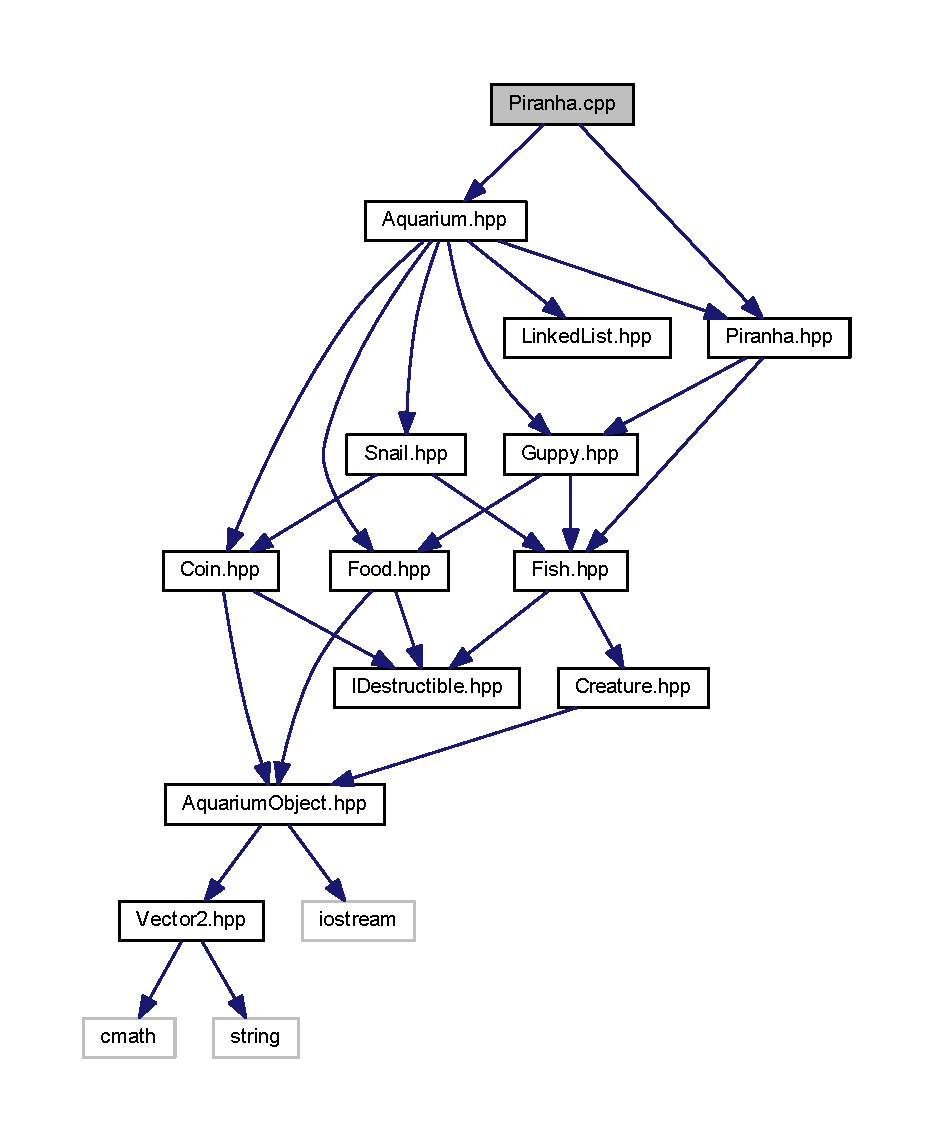
\includegraphics[width=350pt]{_piranha_8cpp__incl}
\end{center}
\end{figure}

\hypertarget{_piranha_8hpp}{}\section{Piranha.\+hpp File Reference}
\label{_piranha_8hpp}\index{Piranha.\+hpp@{Piranha.\+hpp}}
{\ttfamily \#include \char`\"{}Fish.\+hpp\char`\"{}}\newline
{\ttfamily \#include \char`\"{}Guppy.\+hpp\char`\"{}}\newline
Include dependency graph for Piranha.\+hpp\+:\nopagebreak
\begin{figure}[H]
\begin{center}
\leavevmode
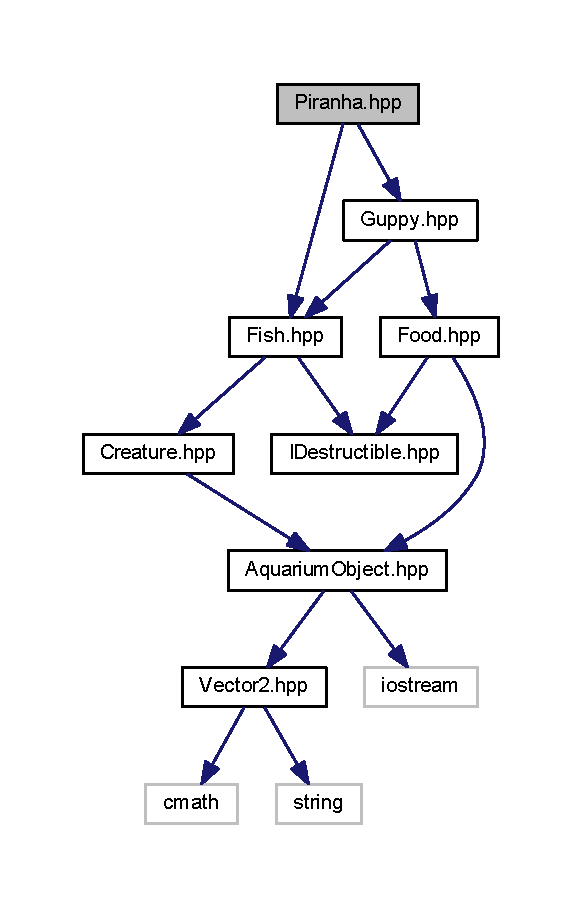
\includegraphics[width=280pt]{_piranha_8hpp__incl}
\end{center}
\end{figure}
This graph shows which files directly or indirectly include this file\+:\nopagebreak
\begin{figure}[H]
\begin{center}
\leavevmode
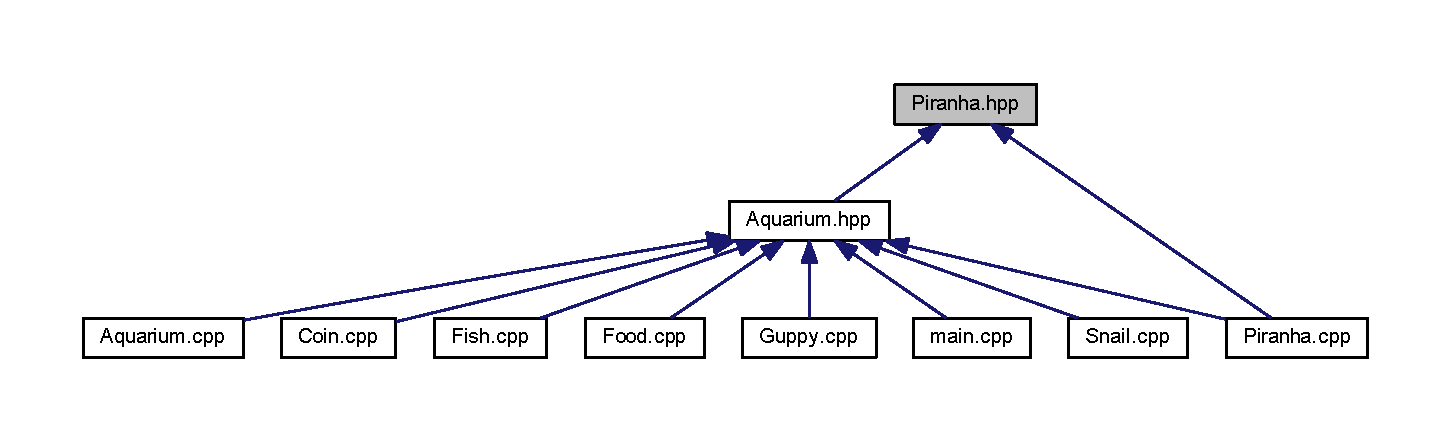
\includegraphics[width=350pt]{_piranha_8hpp__dep__incl}
\end{center}
\end{figure}
\subsection*{Classes}
\begin{DoxyCompactItemize}
\item 
class \mbox{\hyperlink{class_piranha}{Piranha}}
\end{DoxyCompactItemize}

\hypertarget{_snail_8cpp}{}\section{Snail.\+cpp File Reference}
\label{_snail_8cpp}\index{Snail.\+cpp@{Snail.\+cpp}}
{\ttfamily \#include \char`\"{}Snail.\+hpp\char`\"{}}\newline
{\ttfamily \#include \char`\"{}Aquarium.\+hpp\char`\"{}}\newline
Include dependency graph for Snail.\+cpp\+:
\nopagebreak
\begin{figure}[H]
\begin{center}
\leavevmode
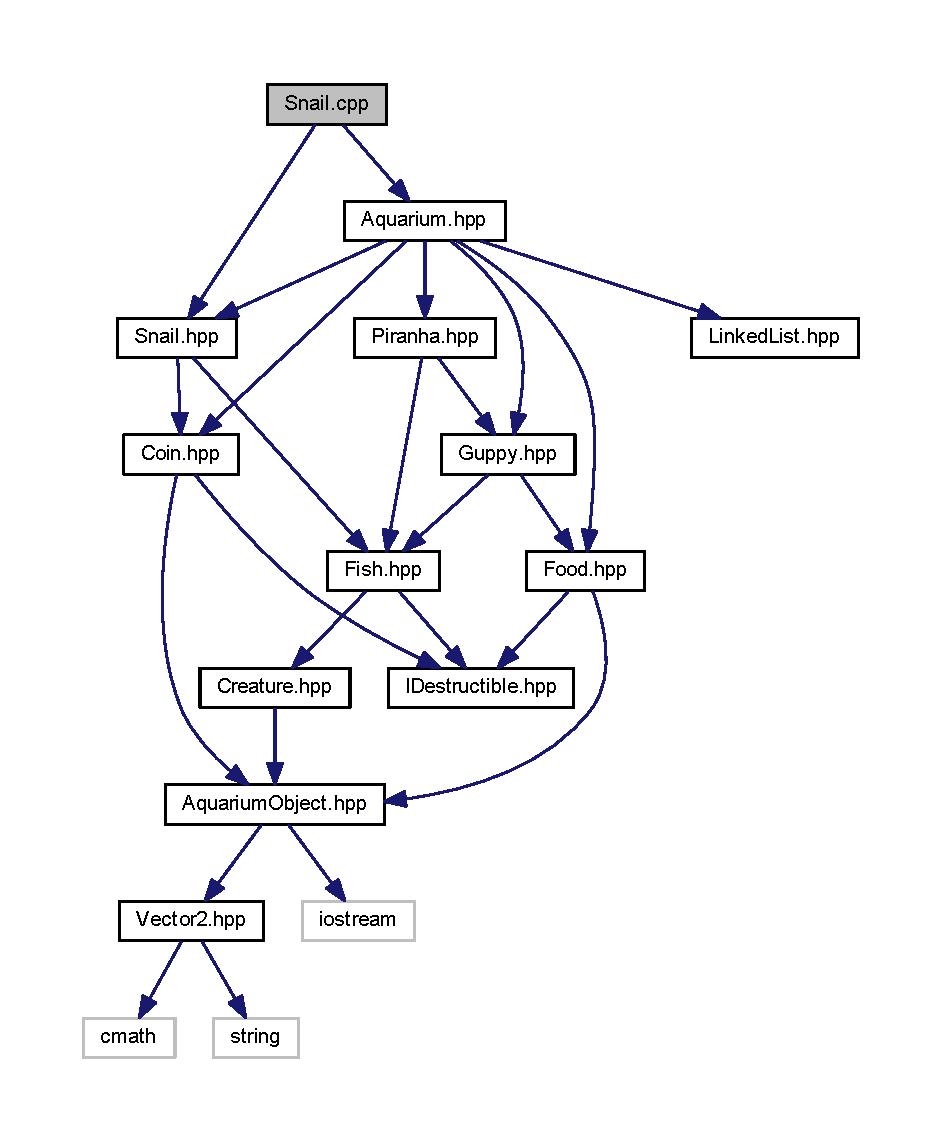
\includegraphics[width=350pt]{_snail_8cpp__incl}
\end{center}
\end{figure}

\hypertarget{_snail_8hpp}{}\section{Snail.\+hpp File Reference}
\label{_snail_8hpp}\index{Snail.\+hpp@{Snail.\+hpp}}
{\ttfamily \#include \char`\"{}Fish.\+hpp\char`\"{}}\newline
{\ttfamily \#include \char`\"{}Coin.\+hpp\char`\"{}}\newline
Include dependency graph for Snail.\+hpp\+:\nopagebreak
\begin{figure}[H]
\begin{center}
\leavevmode
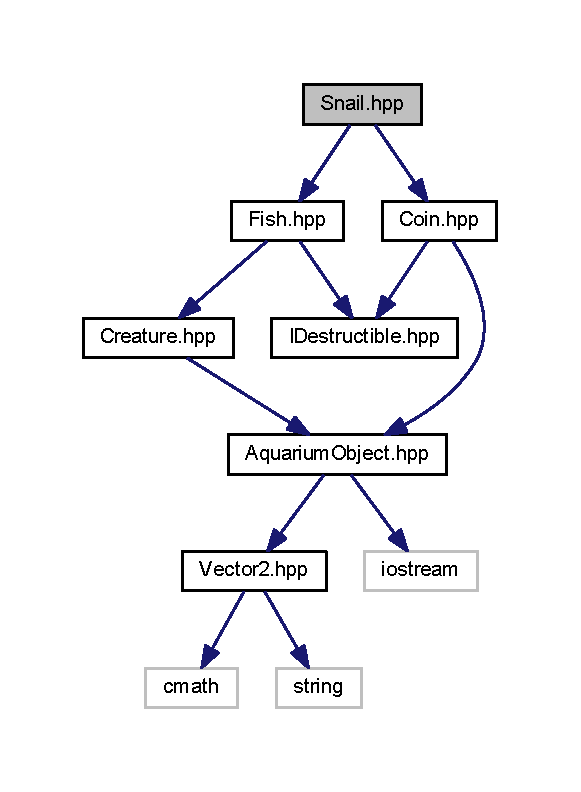
\includegraphics[width=279pt]{_snail_8hpp__incl}
\end{center}
\end{figure}
This graph shows which files directly or indirectly include this file\+:\nopagebreak
\begin{figure}[H]
\begin{center}
\leavevmode
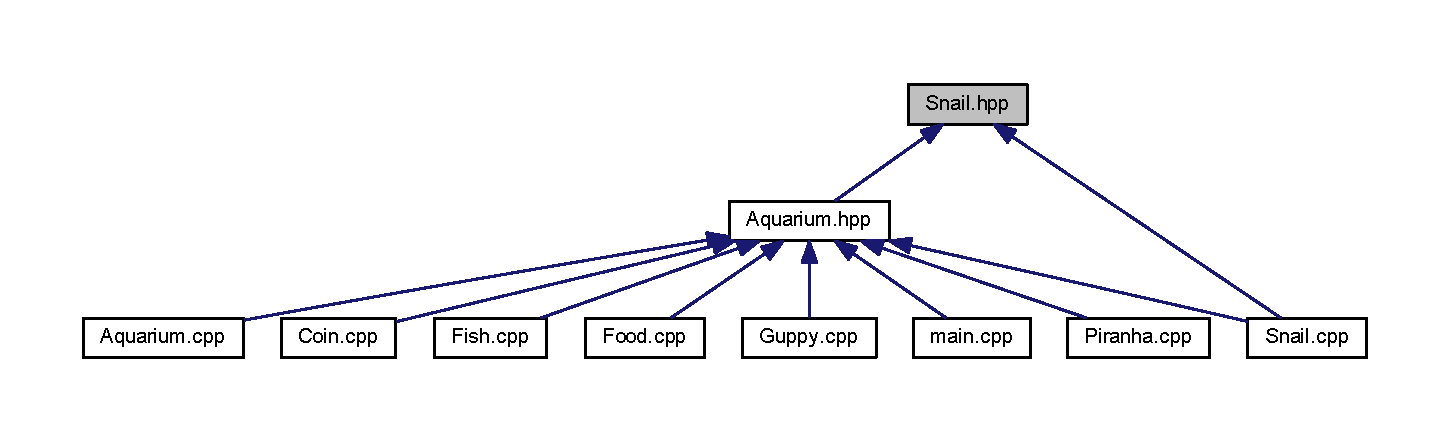
\includegraphics[width=350pt]{_snail_8hpp__dep__incl}
\end{center}
\end{figure}
\subsection*{Classes}
\begin{DoxyCompactItemize}
\item 
class \mbox{\hyperlink{class_snail}{Snail}}
\end{DoxyCompactItemize}

\hypertarget{_vector2_8cpp}{}\section{Vector2.\+cpp File Reference}
\label{_vector2_8cpp}\index{Vector2.\+cpp@{Vector2.\+cpp}}
{\ttfamily \#include \char`\"{}Vector2.\+hpp\char`\"{}}\newline
{\ttfamily \#include $<$cstdlib$>$}\newline
{\ttfamily \#include $<$cmath$>$}\newline
{\ttfamily \#include $<$ctime$>$}\newline
Include dependency graph for Vector2.\+cpp\+:
% FIG 0
\subsection*{Functions}
\begin{DoxyCompactItemize}
\item 
\mbox{\hyperlink{struct_vector2}{Vector2}} \mbox{\hyperlink{_vector2_8cpp_a489f5283f5f1dc905c57d0a40d98c1af}{operator$\ast$}} (\mbox{\hyperlink{struct_vector2}{Vector2}} vector2, double k)
\item 
\mbox{\hyperlink{struct_vector2}{Vector2}} \mbox{\hyperlink{_vector2_8cpp_a6ac6360b23e2a1457b794f0aefc18f3a}{operator$\ast$}} (double k, \mbox{\hyperlink{struct_vector2}{Vector2}} vector2)
\end{DoxyCompactItemize}


\subsection{Function Documentation}
\mbox{\Hypertarget{_vector2_8cpp_a489f5283f5f1dc905c57d0a40d98c1af}\label{_vector2_8cpp_a489f5283f5f1dc905c57d0a40d98c1af}} 
\index{Vector2.\+cpp@{Vector2.\+cpp}!operator$\ast$@{operator$\ast$}}
\index{operator$\ast$@{operator$\ast$}!Vector2.\+cpp@{Vector2.\+cpp}}
\subsubsection{\texorpdfstring{operator$\ast$()}{operator*()}\hspace{0.1cm}{\footnotesize\ttfamily [1/2]}}
{\footnotesize\ttfamily \mbox{\hyperlink{struct_vector2}{Vector2}} operator$\ast$ (\begin{DoxyParamCaption}\item[{\mbox{\hyperlink{struct_vector2}{Vector2}}}]{vector2,  }\item[{double}]{k }\end{DoxyParamCaption})}

\mbox{\Hypertarget{_vector2_8cpp_a6ac6360b23e2a1457b794f0aefc18f3a}\label{_vector2_8cpp_a6ac6360b23e2a1457b794f0aefc18f3a}} 
\index{Vector2.\+cpp@{Vector2.\+cpp}!operator$\ast$@{operator$\ast$}}
\index{operator$\ast$@{operator$\ast$}!Vector2.\+cpp@{Vector2.\+cpp}}
\subsubsection{\texorpdfstring{operator$\ast$()}{operator*()}\hspace{0.1cm}{\footnotesize\ttfamily [2/2]}}
{\footnotesize\ttfamily \mbox{\hyperlink{struct_vector2}{Vector2}} operator$\ast$ (\begin{DoxyParamCaption}\item[{double}]{k,  }\item[{\mbox{\hyperlink{struct_vector2}{Vector2}}}]{vector2 }\end{DoxyParamCaption})}


\hypertarget{_vector2_8hpp}{}\section{Vector2.\+hpp File Reference}
\label{_vector2_8hpp}\index{Vector2.\+hpp@{Vector2.\+hpp}}
{\ttfamily \#include $<$cmath$>$}\newline
{\ttfamily \#include $<$string$>$}\newline
Include dependency graph for Vector2.\+hpp\+:\nopagebreak
\begin{figure}[H]
\begin{center}
\leavevmode
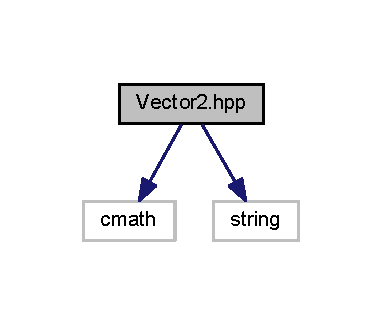
\includegraphics[width=184pt]{_vector2_8hpp__incl}
\end{center}
\end{figure}
This graph shows which files directly or indirectly include this file\+:\nopagebreak
\begin{figure}[H]
\begin{center}
\leavevmode
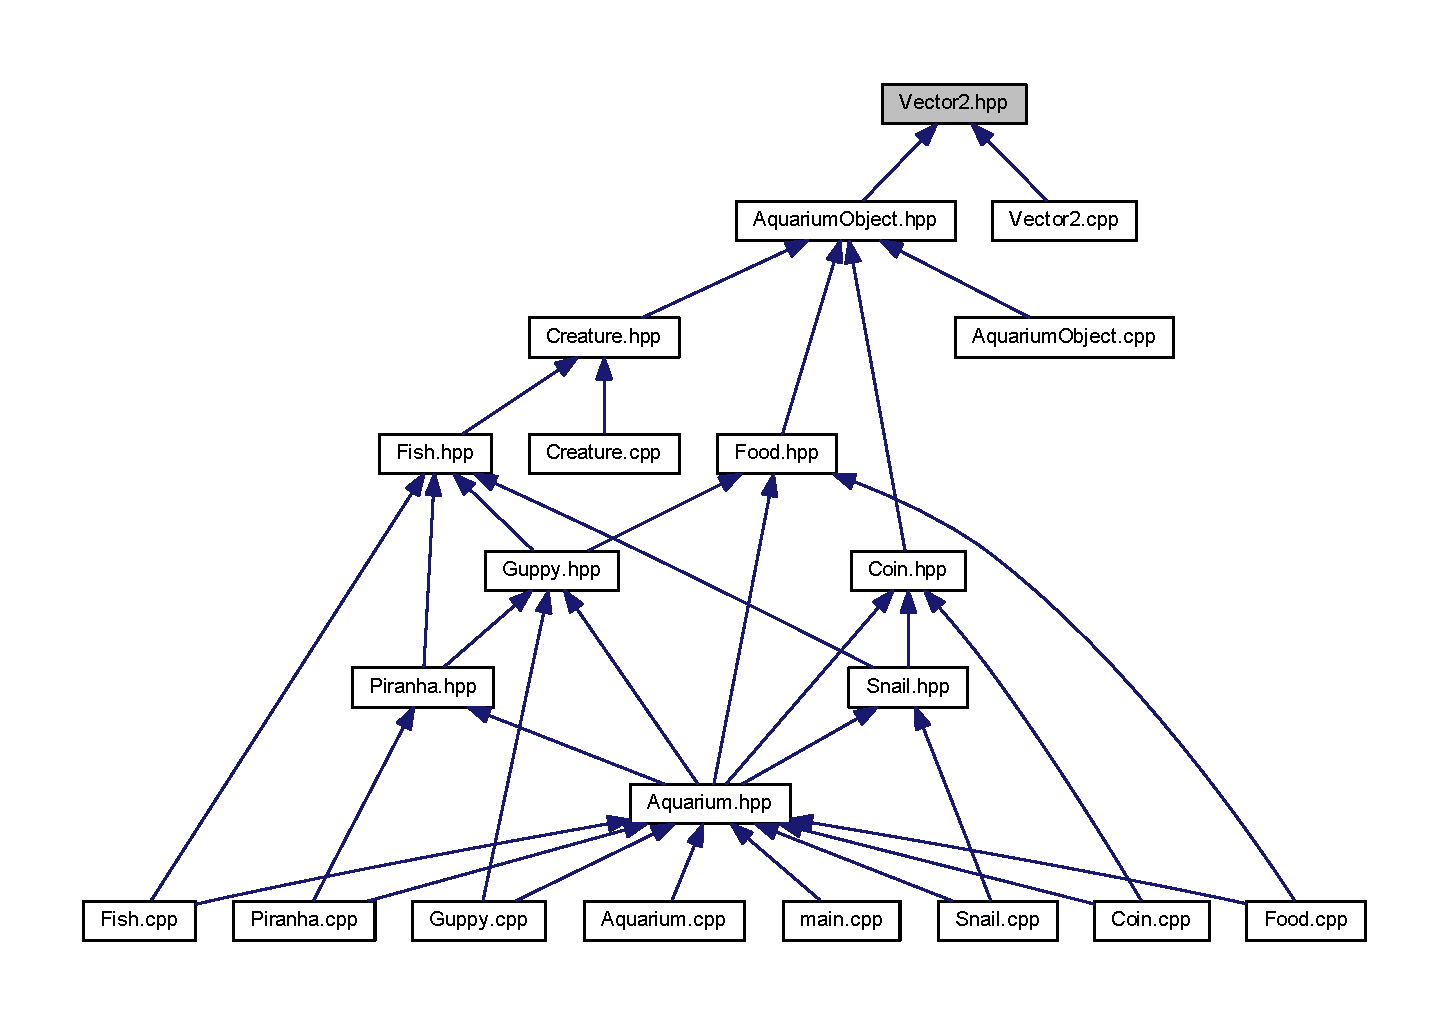
\includegraphics[width=350pt]{_vector2_8hpp__dep__incl}
\end{center}
\end{figure}
\subsection*{Classes}
\begin{DoxyCompactItemize}
\item 
struct \mbox{\hyperlink{struct_vector2}{Vector2}}
\end{DoxyCompactItemize}

%--- End generated contents ---

% Index
\backmatter
\newpage
\phantomsection
\clearemptydoublepage
\addcontentsline{toc}{chapter}{Index}
\printindex

\end{document}
